% Choose the language of your thesis passing 'french' or 'english' as
% \documentclass option.
% Note1: The 'page de garde' will always be written in French.
% Note2: You will have an error if you change the language of the document and
%        compile it without cleaning the auxiliary files. Compiling it again
%        should solve the problem.
\documentclass[english,a4paper,10pt,twoside]{StyleThese}
\newcommand{\included}{}

\usepackage{amsmath,amssymb}             % AMS Math
\usepackage[T1]{fontenc}
\usepackage[utf8x]{inputenc}
\usepackage{babel}
\usepackage{datetime}

\usepackage{lmodern}
\usepackage{tabularx}
%\usepackage{tabular}
\usepackage{multirow}

\usepackage{hhline}
\usepackage[left=1.5in,right=1.3in,top=1.1in,bottom=1.1in,includefoot,includehead,headheight=13.6pt]{geometry}
\renewcommand{\baselinestretch}{1.05}

% Table of contents for each chapter

\usepackage[nottoc, notlof, notlot]{tocbibind}
\usepackage{minitoc}
\setcounter{minitocdepth}{2}
\mtcindent=15pt
% Use \minitoc where to put a table of contents

\usepackage{aecompl}

% Glossary / list of abbreviations

\usepackage[intoc]{nomencl}
\iftoggle{ThesisInEnglish}{%
\renewcommand{\nomname}{Glossary}
}{ %
\renewcommand{\nomname}{Liste des Abréviations}
}

\makenomenclature

% My pdf code

\usepackage{ifpdf}

\ifpdf
  \usepackage[pdftex]{graphicx}
  \DeclareGraphicsExtensions{.jpg}
  \usepackage[a4paper,pagebackref,hyperindex=true]{hyperref}
  \usepackage{tikz}
  \usetikzlibrary{arrows,shapes,calc}
\else
  \usepackage{graphicx}
  \DeclareGraphicsExtensions{.ps,.eps}
  \usepackage[a4paper,dvipdfm,pagebackref,hyperindex=true]{hyperref}
\fi

\graphicspath{{.}{images/}}

%% nicer backref links. NOTE: The flag ThesisInEnglish is used to define the
% language in the back references. Read more about it in These.tex

\iftoggle{ThesisInEnglish}{%
\renewcommand*{\backref}[1]{}
\renewcommand*{\backrefalt}[4]{%
\ifcase #1 %
(Not cited.)%
\or
(Cited in page~#2.)%
\else
(Cited in pages~#2.)%
\fi}
\renewcommand*{\backrefsep}{, }
\renewcommand*{\backreftwosep}{ and~}
\renewcommand*{\backreflastsep}{ and~}
}{%
\renewcommand*{\backref}[1]{}
\renewcommand*{\backrefalt}[4]{%
\ifcase #1 %
(Non cité.)%
\or
(Cité en page~#2.)%
\else
(Cité en pages~#2.)%
\fi}
\renewcommand*{\backrefsep}{, }
\renewcommand*{\backreftwosep}{ et~}
\renewcommand*{\backreflastsep}{ et~}
}

% Links in pdf
\usepackage{color}
\definecolor{linkcol}{rgb}{0,0,0.4} 
\definecolor{citecol}{rgb}{0.5,0,0} 
\definecolor{linkcol}{rgb}{0,0,0} 
\definecolor{citecol}{rgb}{0,0,0}
% Change this to change the informations included in the pdf file

\hypersetup
{
bookmarksopen=true,
pdftitle="Évaluation de la sécurité des équipements grand public connectés à Internet",
pdfauthor="Yann BACHY", %auteur du document
pdfsubject="Thèse", %sujet du document
%pdftoolbar=false, %barre d'outils non visible
pdfmenubar=true, %barre de menu visible
pdfhighlight=/O, %effet d'un clic sur un lien hypertexte
colorlinks=true, %couleurs sur les liens hypertextes
pdfpagemode=None, %aucun mode de page
pdfpagelayout=SinglePage, %ouverture en simple page
pdffitwindow=true, %pages ouvertes entierement dans toute la fenetre
linkcolor=linkcol, %couleur des liens hypertextes internes
citecolor=citecol, %couleur des liens pour les citations
urlcolor=linkcol %couleur des liens pour les url
}

% definitions.
% -------------------

\setcounter{secnumdepth}{3}
\setcounter{tocdepth}{2}

% Some useful commands and shortcut for maths:  partial derivative and stuff

\newcommand{\pd}[2]{\frac{\partial #1}{\partial #2}}
\def\abs{\operatorname{abs}}
\def\argmax{\operatornamewithlimits{arg\,max}}
\def\argmin{\operatornamewithlimits{arg\,min}}
\def\diag{\operatorname{Diag}}
\newcommand{\eqRef}[1]{(\ref{#1})}

\usepackage{rotating}                    % Sideways of figures & tables
%\usepackage{bibunits}
%\usepackage[sectionbib]{chapterbib}          % Cross-reference package (Natural BiB)
%\usepackage{natbib}                  % Put References at the end of each chapter
                                         % Do not put 'sectionbib' option here.
                                         % Sectionbib option in 'natbib' will do.
\usepackage{fancyhdr}                    % Fancy Header and Footer

% \usepackage{txfonts}                     % Public Times New Roman text & math font
  
%%% Fancy Header %%%%%%%%%%%%%%%%%%%%%%%%%%%%%%%%%%%%%%%%%%%%%%%%%%%%%%%%%%%%%%%%%%
% Fancy Header Style Options

\pagestyle{fancy}                       % Sets fancy header and footer
\fancyfoot{}                            % Delete current footer settings

%\renewcommand{\chaptermark}[1]{         % Lower Case Chapter marker style
%  \markboth{\chaptername\ \thechapter.\ #1}}{}} %

%\renewcommand{\sectionmark}[1]{         % Lower case Section marker style
%  \markright{\thesection.\ #1}}         %

\fancyhead[LE,RO]{\bfseries\thepage}    % Page number (boldface) in left on even
% pages and right on odd pages
\fancyhead[RE]{\bfseries\nouppercase{\leftmark}}      % Chapter in the right on even pages
\fancyhead[LO]{\bfseries\nouppercase{\rightmark}}     % Section in the left on odd pages

\let\headruleORIG\headrule
\renewcommand{\headrule}{\color{black} \headruleORIG}
\renewcommand{\headrulewidth}{1.0pt}
\usepackage{colortbl}
\arrayrulecolor{black}

\fancypagestyle{plain}{
  \fancyhead{}
  \fancyfoot{}
  \renewcommand{\headrulewidth}{0pt}
}

%\usepackage{MyAlgorithm}
%\usepackage[noend]{MyAlgorithmic}
\usepackage[ED=MITT - STICRT, Ets=INSA]{tlsflyleaf}
%%% Clear Header %%%%%%%%%%%%%%%%%%%%%%%%%%%%%%%%%%%%%%%%%%%%%%%%%%%%%%%%%%%%%%%%%%
% Clear Header Style on the Last Empty Odd pages
\makeatletter

\def\cleardoublepage{\clearpage\if@twoside \ifodd\c@page\else%
  \hbox{}%
  \thispagestyle{empty}%              % Empty header styles
  \newpage%
  \if@twocolumn\hbox{}\newpage\fi\fi\fi}

\makeatother
 
%%%%%%%%%%%%%%%%%%%%%%%%%%%%%%%%%%%%%%%%%%%%%%%%%%%%%%%%%%%%%%%%%%%%%%%%%%%%%%% 
% Prints your review date and 'Draft Version' (From Josullvn, CS, CMU)
\newcommand{\reviewtimetoday}[2]{\special{!userdict begin
    /bop-hook{gsave 20 710 translate 45 rotate 0.8 setgray
      /Times-Roman findfont 12 scalefont setfont 0 0   moveto (#1) show
      0 -12 moveto (#2) show grestore}def end}}
% You can turn on or off this option.
% \reviewtimetoday{\today}{Draft Version}
%%%%%%%%%%%%%%%%%%%%%%%%%%%%%%%%%%%%%%%%%%%%%%%%%%%%%%%%%%%%%%%%%%%%%%%%%%%%%%% 

\newenvironment{maxime}[1]
{
\vspace*{0cm}
\hfill
\begin{minipage}{0.5\textwidth}%
%\rule[0.5ex]{\textwidth}{0.1mm}\\%
\hrulefill $\:$ {\bf #1}\\
%\vspace*{-0.25cm}
\it 
}%
{%

\hrulefill
\vspace*{0.5cm}%
\end{minipage}
}

\let\minitocORIG\minitoc
\renewcommand{\minitoc}{\minitocORIG \vspace{1.5em}}

\usepackage{multirow}
%\usepackage{slashbox}

\newenvironment{bulletList}%
{ \begin{list}%
	{$\bullet$}%
	{\setlength{\labelwidth}{25pt}%
	 \setlength{\leftmargin}{30pt}%
	 \setlength{\itemsep}{\parsep}}}%
{ \end{list} }

\newtheorem{definition}{Définition}
\renewcommand{\epsilon}{\varepsilon}

% centered page environment

\newenvironment{vcenterpage}
{\newpage\vspace*{\fill}\thispagestyle{empty}\renewcommand{\headrulewidth}{0pt}}
{\vspace*{\fill}}

\usepackage{tablefootnote}

\usepackage{hyperref}
\hypersetup{
     colorlinks   = true,
     citecolor    = violet
}
\usepackage{graphicx} % for pdf, bitmapped graphics files
\usepackage{amsmath} % assumes amsmath package installed
\usepackage{amssymb}  % assumes amsmath package installed
\usepackage{bm} % for using bold lowercase greek letters
\usepackage{array}
\usepackage{colortbl}	% to color table background
%\usepackage[table]{xcolor}
\usepackage{subfigure}  
\usepackage{tikz}
\newcommand{\tikzcircle}[2][red,fill=red]{\tikz[baseline=-0.5ex]\draw[#1,radius=#2] (0,0) circle ;}%
\definecolor{turquoise}{rgb}{0.28 1 0.92}
\newcommand{\fratop}[2]{\genfrac{}{}{0pt}{}{#1}{#2}}
\newcommand{\mx}[1]{\mathbf{\bm{#1}}} 				% Matrix symbol
\newcommand{\vc}[1]{\mathbf{\bm{#1}}} 					% Vector symbol
\newcommand{\degree}{\ensuremath{^\circ}}				% define the degree symbol
\newcommand{\pder}[2]{\frac{\partial#1}{\partial#2}}		% partial derivative
\newcommand{\ppder}[2]{\frac{\partial^2 #1}{\partial#2^2}}		% second partial derivative
\newcommand{\refframe}[1]{\mbox{\textless#1\textgreater}}	% to denote a reference frame
%\DeclareMathOperator*{\lexmin}{\text{lex}\!\min}			% lexmin
\DeclareMathOperator*{\minimize}{minimize}				% minimize
\DeclareMathOperator*{\maximize}{maximize}				% maximize
%\DeclareMathOperator*{\argmin}{\arg\!\min}				% argmin
%\DeclareMathOperator*{\argmax}{\arg\!\max}				% argmax
\DeclareMathOperator*{\st}{subject\,to}					% subject to
\DeclareMathOperator*{\dif}{\mathrm{d}}					% d
\DeclareMathOperator*{\half}{\frac{1}{2}}					% one half
\newcommand{\mat}[1]{\ensuremath{\begin{bmatrix}#1\end{bmatrix}}}	% matrix
\newcommand{\rank}[1]{\text{rank}(#1)}							% rank
%\newcommand{\diag}[1]{\text{diag}(#1)}							% diag
\newcommand{\x}{\ensuremath{\times}}
\newcommand{\spac}{\ensuremath{\quad}}						% alias for space in math environment
\newcommand{\dt}[0]{\ensuremath{\Delta t}}					% dt
\newcommand{\dx}[0]{\ensuremath{\delta x}}					% dx
\newcommand{\du}[0]{\ensuremath{\delta u}}					% du
\newcommand{\dhu}[0]{\ensuremath{\delta \hat{u}}}					% \hat{du}
\newcommand{\dbu}[0]{\ensuremath{\delta \bar{u}}}					% \bar{du}
\newcommand{\dtu}[0]{\ensuremath{\delta \tilde{u}}}					% \tilde{du}
\newcommand{\dhx}[0]{\ensuremath{\delta \hat{x}}}					% \hat{dx}
\newcommand{\DX}[0]{\ensuremath{\Delta X}}						% DX
\newcommand{\DU}[0]{\ensuremath{\Delta U}}						% DU
\newcommand{\Ts}[0]{\ensuremath{\top}}							% transpose symbol
\newcommand{\pinv}[0]{\ensuremath{\dagger}}					% pseudoinverse symbol
\newcommand{\Rv}[1]{\ensuremath{\mathbb{R}^{#1}}}				% set of real-valued vectors
\newcommand{\Rm}[2]{\ensuremath{\mathbb{R}^{#1\times #2}}}		% set of real-valued matrices
\newcommand{\Spd}[1]{\ensuremath{\mathbb{S}_+^{#1}}}			% set of symmetric positive-definite matrices
\newcommand{\card}[1]{\ensuremath{\left\vert{#1}\right\vert}}			% cardinality of a set
\DeclareMathOperator{\Tr}{Tr}							% trace
\newcommand{\Expect}{{\rm I\kern-.3em E}}				% expectation
\newcommand{\Normal}{\mathcal{N}}					% normal distribution
\newcommand{\Prob}[1]{\text{P}(#1)}						% probability
\newcommand{\vech}[1]{\text{vech}(#1)}						% vech

\newcommand{\sethree}{\ensuremath{SE(3)}}
\newcommand{\CS}{$\mathcal{CS}$}
\newcommand{\WS}{$\mathcal{WS}$}
\newcommand{\CSfree}{$\mathcal{CS}_{free}$}
\newcommand{\CSobst}{$\mathcal{CS}_{obst}$}
\newcommand{\M}[0]{$\mathcal{M}$}

%\algnewcommand{\algorithmicgoto}{\textbf{go to}}%
%%\algnewcommand{\Goto}[1]{\algorithmicgoto~\ref{#1}}%
%\algnewcommand{\Goto}{\algorithmicgoto\xspace}%
%\algnewcommand{\Label}{\State\unskip}

\newenvironment{definition}[1][Definition]{\begin{trivlist}
\item[\hskip \labelsep {\bfseries #1}]}{\end{trivlist}}

\usepackage{epstopdf}
\usepackage[colorinlistoftodos,prependcaption,textsize=tiny]{todonotes}
\newcommand\explainmore[1]{\textcolor{red}{#1}}
\newcommand\refrephrase[1]{\textcolor{yellow}{#1}}
\newcommand\donerephrasing[1]{\textcolor{green}{#1}}

%DIF PREAMBLE EXTENSION ADDED BY LATEXDIFF
%DIF UNDERLINE PREAMBLE %DIF PREAMBLE
\RequirePackage[normalem]{ulem} %DIF PREAMBLE
\RequirePackage{color}\definecolor{RED}{rgb}{1,0,0}\definecolor{BLUE}{rgb}{0,0,1} %DIF PREAMBLE
\providecommand{\DIFadd}[1]{{\protect\color{blue}\uwave{#1}}} %DIF PREAMBLE
\providecommand{\DIFdel}[1]{{\protect\color{red}\sout{#1}}}                      %DIF PREAMBLE
%DIF SAFE PREAMBLE %DIF PREAMBLE
\providecommand{\DIFaddbegin}{} %DIF PREAMBLE
\providecommand{\DIFaddend}{} %DIF PREAMBLE
\providecommand{\DIFdelbegin}{} %DIF PREAMBLE
\providecommand{\DIFdelend}{} %DIF PREAMBLE
%DIF FLOATSAFE PREAMBLE %DIF PREAMBLE
\providecommand{\DIFaddFL}[1]{\DIFadd{#1}} %DIF PREAMBLE
\providecommand{\DIFdelFL}[1]{\DIFdel{#1}} %DIF PREAMBLE
\providecommand{\DIFaddbeginFL}{} %DIF PREAMBLE
\providecommand{\DIFaddendFL}{} %DIF PREAMBLE
\providecommand{\DIFdelbeginFL}{} %DIF PREAMBLE
\providecommand{\DIFdelendFL}{} %DIF PREAMBLE
%DIF END PREAMBLE EXTENSION ADDED BY LATEXDIFF


\begin{document}


\sloppy
\begin{document}
    
%% This is file `example.tex',
%% Copyright 2013 Tristan GREGOIRE
%% Copyright 2015 Yann BACHY
%
% This work may be distributed and/or modified under the
% conditions of the LaTeX Project Public License, either version 1.3
% of this license or (at your option) any later version.
% The latest version of this license is in
%   http://www.latex-project.org/lppl.txt
% and version 1.3 or later is part of all distributions of LaTeX
% version 2005/12/01 or later.
%
%
% This work has the LPPL maintenance status `maintained'.
% 
% The Current Maintainer of this work is T. GREGOIRE
%

%\documentclass{book}

% Loading the tlsflyleaf.sty package require some option to define the
% establishment name, the doctoral school and the PhD speciality.
% In that aim you have 2 key-value option:
%   - Ets=<value> : define the establishment name
%   - ED=<value>  : define the doctoral school and speciality
%   - ED2=<value> : define the second speciality ("double mention"). OPTIONAL.
% The full list of accepted values for each option could be find either
% in the documentation or in ED-list.txt and Ets-list.txt files provide with the package.
%  \doubleSpe{EDSYS : Robotique 4200046}
 \docschool{EDSYS : Robotique 4200046}
% \establishment{l'Institut National des Sciences Appliqu\'ees de Toulouse (INSA de Toulouse)}
% ==================
% Setup basic string
% - PhD Title
% - author
% - defence date
% - laboratory
% - cotutelle
\title{\textbf{\large Handling Uncertainty and Variability in Robot Control}}
\author{Nirmal GIFTSUN}
\defencedate{28/10/2017}
\lab{Laboratoire d'analyse et d'architecture des systèmes(LAAS)}
%\cotutelle{}

% ==================
% Setup people like your boss, the jury team and the referees
% - First you need to define how number they will be in each category
%   It is done with the commands \nboss{n}, \nreferee{n} and \njudge{n}.
%   You can define more people in each category than the number given 
%   but only the first "\npeople" will be print.
% - Then use the command \makesomeone{<category>}{<number>}{<name>}{<status>}{<other>}
%   where:
%     <category> should be select in ['boss', 'referee', 'judge']
%     <number>   is the rank for printing the person. 
%                Only number <= "\npeople" will be printed
%     <name>     First name and las name of the people
%     <status>   Is (s)he a "charg\'e de recher" ou un "professeur d'universit\'e"...
%     <other>    What ever string you want to add (laboratory, jury member place...).
%% Boss
\nboss{2}
\makesomeone{boss}{2}{Andrea DEL PRETE}{}{}  % Sera affiche en second
\makesomeone{boss}{1}{Florent LAMIRAUX}{}{} % Sera afiche en premier
%% Referee
\nreferee{2}
\makesomeone{referee}{1}{Vincent PADOIS}{}{}
\makesomeone{referee}{2}{Paul PLOEGER}{}{}
%% Judges
\njudge{5}
\makesomeone{judge}{1}{Vincent PADOIS}{Professeur d'Universit\'e}{Rapporteur}
\makesomeone{judge}{2}{Paul PLOEGER}{Astronome Adjoint}{Rapporteur}
\makesomeone{judge}{3}{Florent LAMIRAUX}{Directeur de Recherche}{Directeur de thèse}
\makesomeone{judge}{4}{Andrea DEL PRETE}{Chercheur}{Codirecteur de thèse}
% \makesomeone{judge}{5}{Ciqui\`eme MEMBRE}{Charg\'e de Recherche}{Membre du Jury}

% ============================================================
% DOCUMENT
%\begin{document}
%    \makeflyleaf
%\end{document}


\makeflyleaf

\cleardoublepage

\dominitoc

\pagenumbering{roman}

\cleardoublepage

% \iftoggle{ThesisInEnglish}{%
% \section*{Acknowledgments}
% }{%
% \section*{Remerciements}
% }
% A faire en dernier :-) 

\begin{vcenterpage}
\iftoggle{ThesisInEnglish}{%
\section*{Abstract}
}{%
\section*{Resume}
}
Amidst a lot of research in motion planning and control in concern with robotic applications, the mankind has never reached a point yet, where the robots are perfectly functional and autonomous in dynamic settings. Though it is controversial to discuss about the necessity of such robots, it is very important to address the issues that stop us from achieving such a level of autonomy. Industrial robots have evolved to be very reliable and highly productive with more than 1.5 million operation robots in a variety of industries. These robots work in static settings and they literally do what it is programmed for specific usecases, though the robots are flexible enough to be programmed for a variety of tasks. This research work makes an attempt to address these issues that separate both these settings in a profound way with special focus on uncertainties. Practical impossibilities of precise sensing abilities lead to a variety of uncertainties in scenarios where the robot is mobile or the environment is dynamic. This work focuses on developing smart strategies to improve the ability to handle uncertainties robustly in humanoid and industrial robots. First, we focus on a dynamical obstacle avoidance framework proposed for industrial robots equipped with skin sensors for reactivity. Path planning and motion control are usually formalized as separate problems in robotics, though both fundamentally address the same issue. High dimensional configuration spaces, changing environment and uncertainties do not allow to plan real-time motion ahead of time requiring a controller to execute the planned trajectory. The fundamental inability to unify both these problems has led to handle the planned trajectory amidst perturbations and unforeseen obstacles using various trajectory execution and deformation mechanisms. The proposed framework uses 'Stack of Tasks', a hierarchical controller using proximity information with a point cloud based reactive path planner to avoid obstacles. Experiments are performed in PR2 and UR5 robot to check the validity of the framework both in simulation and real robot.

 Second, we focus on a strategy to model uncertainties in the inertial parameters of a humanoid robot in a balancing task scenarios. Model-based control has become more and more popular in the legged robots community in the last ten years. The key idea is to exploit a model of the system to compute precise motor commands that result in the desired motion. This allows to improve the quality of the motion tracking, while using lower feedback gains, leading so to higher compliance. However, the main flaw of this approach is typically its lack of robustness to modeling errors. In this paper we focus on the robustness of inverse-dynamics control to errors in the inertial parameters of the robot. We assume these parameters to be known, but only with a certain accuracy. We then propose a computationally-efficient optimization-based controller that ensures the balance of the robot despite these uncertainties. We used the proposed controller in simulation to perform different reaching tasks with the HRP-2 humanoid robot, in the presence of various modeling errors. Comparisons against a standard inverse-dynamics controller through hundreds of simulations show the superiority of the proposed controller in ensuring the robot balance.
\end{vcenterpage}

\tableofcontents
\printnomenclature
\mtcfixnomenclature
\mainmatter
% \ifdefined\included
\else
\documentclass[a4paper,11pt,twoside]{StyleThese}
\usepackage{amsmath,amssymb}             % AMS Math
\usepackage[T1]{fontenc}
\usepackage[utf8x]{inputenc}
\usepackage{babel}
\usepackage{datetime}

\usepackage{lmodern}
\usepackage{tabularx}
%\usepackage{tabular}
\usepackage{multirow}

\usepackage{hhline}
\usepackage[left=1.5in,right=1.3in,top=1.1in,bottom=1.1in,includefoot,includehead,headheight=13.6pt]{geometry}
\renewcommand{\baselinestretch}{1.05}

% Table of contents for each chapter

\usepackage[nottoc, notlof, notlot]{tocbibind}
\usepackage{minitoc}
\setcounter{minitocdepth}{2}
\mtcindent=15pt
% Use \minitoc where to put a table of contents

\usepackage{aecompl}

% Glossary / list of abbreviations

\usepackage[intoc]{nomencl}
\iftoggle{ThesisInEnglish}{%
\renewcommand{\nomname}{Glossary}
}{ %
\renewcommand{\nomname}{Liste des Abréviations}
}

\makenomenclature

% My pdf code

\usepackage{ifpdf}

\ifpdf
  \usepackage[pdftex]{graphicx}
  \DeclareGraphicsExtensions{.jpg}
  \usepackage[a4paper,pagebackref,hyperindex=true]{hyperref}
  \usepackage{tikz}
  \usetikzlibrary{arrows,shapes,calc}
\else
  \usepackage{graphicx}
  \DeclareGraphicsExtensions{.ps,.eps}
  \usepackage[a4paper,dvipdfm,pagebackref,hyperindex=true]{hyperref}
\fi

\graphicspath{{.}{images/}}

%% nicer backref links. NOTE: The flag ThesisInEnglish is used to define the
% language in the back references. Read more about it in These.tex

\iftoggle{ThesisInEnglish}{%
\renewcommand*{\backref}[1]{}
\renewcommand*{\backrefalt}[4]{%
\ifcase #1 %
(Not cited.)%
\or
(Cited in page~#2.)%
\else
(Cited in pages~#2.)%
\fi}
\renewcommand*{\backrefsep}{, }
\renewcommand*{\backreftwosep}{ and~}
\renewcommand*{\backreflastsep}{ and~}
}{%
\renewcommand*{\backref}[1]{}
\renewcommand*{\backrefalt}[4]{%
\ifcase #1 %
(Non cité.)%
\or
(Cité en page~#2.)%
\else
(Cité en pages~#2.)%
\fi}
\renewcommand*{\backrefsep}{, }
\renewcommand*{\backreftwosep}{ et~}
\renewcommand*{\backreflastsep}{ et~}
}

% Links in pdf
\usepackage{color}
\definecolor{linkcol}{rgb}{0,0,0.4} 
\definecolor{citecol}{rgb}{0.5,0,0} 
\definecolor{linkcol}{rgb}{0,0,0} 
\definecolor{citecol}{rgb}{0,0,0}
% Change this to change the informations included in the pdf file

\hypersetup
{
bookmarksopen=true,
pdftitle="Évaluation de la sécurité des équipements grand public connectés à Internet",
pdfauthor="Yann BACHY", %auteur du document
pdfsubject="Thèse", %sujet du document
%pdftoolbar=false, %barre d'outils non visible
pdfmenubar=true, %barre de menu visible
pdfhighlight=/O, %effet d'un clic sur un lien hypertexte
colorlinks=true, %couleurs sur les liens hypertextes
pdfpagemode=None, %aucun mode de page
pdfpagelayout=SinglePage, %ouverture en simple page
pdffitwindow=true, %pages ouvertes entierement dans toute la fenetre
linkcolor=linkcol, %couleur des liens hypertextes internes
citecolor=citecol, %couleur des liens pour les citations
urlcolor=linkcol %couleur des liens pour les url
}

% definitions.
% -------------------

\setcounter{secnumdepth}{3}
\setcounter{tocdepth}{2}

% Some useful commands and shortcut for maths:  partial derivative and stuff

\newcommand{\pd}[2]{\frac{\partial #1}{\partial #2}}
\def\abs{\operatorname{abs}}
\def\argmax{\operatornamewithlimits{arg\,max}}
\def\argmin{\operatornamewithlimits{arg\,min}}
\def\diag{\operatorname{Diag}}
\newcommand{\eqRef}[1]{(\ref{#1})}

\usepackage{rotating}                    % Sideways of figures & tables
%\usepackage{bibunits}
%\usepackage[sectionbib]{chapterbib}          % Cross-reference package (Natural BiB)
%\usepackage{natbib}                  % Put References at the end of each chapter
                                         % Do not put 'sectionbib' option here.
                                         % Sectionbib option in 'natbib' will do.
\usepackage{fancyhdr}                    % Fancy Header and Footer

% \usepackage{txfonts}                     % Public Times New Roman text & math font
  
%%% Fancy Header %%%%%%%%%%%%%%%%%%%%%%%%%%%%%%%%%%%%%%%%%%%%%%%%%%%%%%%%%%%%%%%%%%
% Fancy Header Style Options

\pagestyle{fancy}                       % Sets fancy header and footer
\fancyfoot{}                            % Delete current footer settings

%\renewcommand{\chaptermark}[1]{         % Lower Case Chapter marker style
%  \markboth{\chaptername\ \thechapter.\ #1}}{}} %

%\renewcommand{\sectionmark}[1]{         % Lower case Section marker style
%  \markright{\thesection.\ #1}}         %

\fancyhead[LE,RO]{\bfseries\thepage}    % Page number (boldface) in left on even
% pages and right on odd pages
\fancyhead[RE]{\bfseries\nouppercase{\leftmark}}      % Chapter in the right on even pages
\fancyhead[LO]{\bfseries\nouppercase{\rightmark}}     % Section in the left on odd pages

\let\headruleORIG\headrule
\renewcommand{\headrule}{\color{black} \headruleORIG}
\renewcommand{\headrulewidth}{1.0pt}
\usepackage{colortbl}
\arrayrulecolor{black}

\fancypagestyle{plain}{
  \fancyhead{}
  \fancyfoot{}
  \renewcommand{\headrulewidth}{0pt}
}

%\usepackage{MyAlgorithm}
%\usepackage[noend]{MyAlgorithmic}
\usepackage[ED=MITT - STICRT, Ets=INSA]{tlsflyleaf}
%%% Clear Header %%%%%%%%%%%%%%%%%%%%%%%%%%%%%%%%%%%%%%%%%%%%%%%%%%%%%%%%%%%%%%%%%%
% Clear Header Style on the Last Empty Odd pages
\makeatletter

\def\cleardoublepage{\clearpage\if@twoside \ifodd\c@page\else%
  \hbox{}%
  \thispagestyle{empty}%              % Empty header styles
  \newpage%
  \if@twocolumn\hbox{}\newpage\fi\fi\fi}

\makeatother
 
%%%%%%%%%%%%%%%%%%%%%%%%%%%%%%%%%%%%%%%%%%%%%%%%%%%%%%%%%%%%%%%%%%%%%%%%%%%%%%% 
% Prints your review date and 'Draft Version' (From Josullvn, CS, CMU)
\newcommand{\reviewtimetoday}[2]{\special{!userdict begin
    /bop-hook{gsave 20 710 translate 45 rotate 0.8 setgray
      /Times-Roman findfont 12 scalefont setfont 0 0   moveto (#1) show
      0 -12 moveto (#2) show grestore}def end}}
% You can turn on or off this option.
% \reviewtimetoday{\today}{Draft Version}
%%%%%%%%%%%%%%%%%%%%%%%%%%%%%%%%%%%%%%%%%%%%%%%%%%%%%%%%%%%%%%%%%%%%%%%%%%%%%%% 

\newenvironment{maxime}[1]
{
\vspace*{0cm}
\hfill
\begin{minipage}{0.5\textwidth}%
%\rule[0.5ex]{\textwidth}{0.1mm}\\%
\hrulefill $\:$ {\bf #1}\\
%\vspace*{-0.25cm}
\it 
}%
{%

\hrulefill
\vspace*{0.5cm}%
\end{minipage}
}

\let\minitocORIG\minitoc
\renewcommand{\minitoc}{\minitocORIG \vspace{1.5em}}

\usepackage{multirow}
%\usepackage{slashbox}

\newenvironment{bulletList}%
{ \begin{list}%
	{$\bullet$}%
	{\setlength{\labelwidth}{25pt}%
	 \setlength{\leftmargin}{30pt}%
	 \setlength{\itemsep}{\parsep}}}%
{ \end{list} }

\newtheorem{definition}{Définition}
\renewcommand{\epsilon}{\varepsilon}

% centered page environment

\newenvironment{vcenterpage}
{\newpage\vspace*{\fill}\thispagestyle{empty}\renewcommand{\headrulewidth}{0pt}}
{\vspace*{\fill}}

\usepackage{tablefootnote}

\usepackage{hyperref}
\hypersetup{
     colorlinks   = true,
     citecolor    = violet
}
\usepackage{graphicx} % for pdf, bitmapped graphics files
\usepackage{amsmath} % assumes amsmath package installed
\usepackage{amssymb}  % assumes amsmath package installed
\usepackage{bm} % for using bold lowercase greek letters
\usepackage{array}
\usepackage{colortbl}	% to color table background
%\usepackage[table]{xcolor}
\usepackage{subfigure}  
\usepackage{tikz}
\newcommand{\tikzcircle}[2][red,fill=red]{\tikz[baseline=-0.5ex]\draw[#1,radius=#2] (0,0) circle ;}%
\definecolor{turquoise}{rgb}{0.28 1 0.92}
\newcommand{\fratop}[2]{\genfrac{}{}{0pt}{}{#1}{#2}}
\newcommand{\mx}[1]{\mathbf{\bm{#1}}} 				% Matrix symbol
\newcommand{\vc}[1]{\mathbf{\bm{#1}}} 					% Vector symbol
\newcommand{\degree}{\ensuremath{^\circ}}				% define the degree symbol
\newcommand{\pder}[2]{\frac{\partial#1}{\partial#2}}		% partial derivative
\newcommand{\ppder}[2]{\frac{\partial^2 #1}{\partial#2^2}}		% second partial derivative
\newcommand{\refframe}[1]{\mbox{\textless#1\textgreater}}	% to denote a reference frame
%\DeclareMathOperator*{\lexmin}{\text{lex}\!\min}			% lexmin
\DeclareMathOperator*{\minimize}{minimize}				% minimize
\DeclareMathOperator*{\maximize}{maximize}				% maximize
%\DeclareMathOperator*{\argmin}{\arg\!\min}				% argmin
%\DeclareMathOperator*{\argmax}{\arg\!\max}				% argmax
\DeclareMathOperator*{\st}{subject\,to}					% subject to
\DeclareMathOperator*{\dif}{\mathrm{d}}					% d
\DeclareMathOperator*{\half}{\frac{1}{2}}					% one half
\newcommand{\mat}[1]{\ensuremath{\begin{bmatrix}#1\end{bmatrix}}}	% matrix
\newcommand{\rank}[1]{\text{rank}(#1)}							% rank
%\newcommand{\diag}[1]{\text{diag}(#1)}							% diag
\newcommand{\x}{\ensuremath{\times}}
\newcommand{\spac}{\ensuremath{\quad}}						% alias for space in math environment
\newcommand{\dt}[0]{\ensuremath{\Delta t}}					% dt
\newcommand{\dx}[0]{\ensuremath{\delta x}}					% dx
\newcommand{\du}[0]{\ensuremath{\delta u}}					% du
\newcommand{\dhu}[0]{\ensuremath{\delta \hat{u}}}					% \hat{du}
\newcommand{\dbu}[0]{\ensuremath{\delta \bar{u}}}					% \bar{du}
\newcommand{\dtu}[0]{\ensuremath{\delta \tilde{u}}}					% \tilde{du}
\newcommand{\dhx}[0]{\ensuremath{\delta \hat{x}}}					% \hat{dx}
\newcommand{\DX}[0]{\ensuremath{\Delta X}}						% DX
\newcommand{\DU}[0]{\ensuremath{\Delta U}}						% DU
\newcommand{\Ts}[0]{\ensuremath{\top}}							% transpose symbol
\newcommand{\pinv}[0]{\ensuremath{\dagger}}					% pseudoinverse symbol
\newcommand{\Rv}[1]{\ensuremath{\mathbb{R}^{#1}}}				% set of real-valued vectors
\newcommand{\Rm}[2]{\ensuremath{\mathbb{R}^{#1\times #2}}}		% set of real-valued matrices
\newcommand{\Spd}[1]{\ensuremath{\mathbb{S}_+^{#1}}}			% set of symmetric positive-definite matrices
\newcommand{\card}[1]{\ensuremath{\left\vert{#1}\right\vert}}			% cardinality of a set
\DeclareMathOperator{\Tr}{Tr}							% trace
\newcommand{\Expect}{{\rm I\kern-.3em E}}				% expectation
\newcommand{\Normal}{\mathcal{N}}					% normal distribution
\newcommand{\Prob}[1]{\text{P}(#1)}						% probability
\newcommand{\vech}[1]{\text{vech}(#1)}						% vech

\newcommand{\sethree}{\ensuremath{SE(3)}}
\newcommand{\CS}{$\mathcal{CS}$}
\newcommand{\WS}{$\mathcal{WS}$}
\newcommand{\CSfree}{$\mathcal{CS}_{free}$}
\newcommand{\CSobst}{$\mathcal{CS}_{obst}$}
\newcommand{\M}[0]{$\mathcal{M}$}

%\algnewcommand{\algorithmicgoto}{\textbf{go to}}%
%%\algnewcommand{\Goto}[1]{\algorithmicgoto~\ref{#1}}%
%\algnewcommand{\Goto}{\algorithmicgoto\xspace}%
%\algnewcommand{\Label}{\State\unskip}

\newenvironment{definition}[1][Definition]{\begin{trivlist}
\item[\hskip \labelsep {\bfseries #1}]}{\end{trivlist}}

\usepackage{epstopdf}
\usepackage[colorinlistoftodos,prependcaption,textsize=tiny]{todonotes}
\newcommand\explainmore[1]{\textcolor{red}{#1}}
\newcommand\refrephrase[1]{\textcolor{yellow}{#1}}
\newcommand\donerephrasing[1]{\textcolor{green}{#1}}

%DIF PREAMBLE EXTENSION ADDED BY LATEXDIFF
%DIF UNDERLINE PREAMBLE %DIF PREAMBLE
\RequirePackage[normalem]{ulem} %DIF PREAMBLE
\RequirePackage{color}\definecolor{RED}{rgb}{1,0,0}\definecolor{BLUE}{rgb}{0,0,1} %DIF PREAMBLE
\providecommand{\DIFadd}[1]{{\protect\color{blue}\uwave{#1}}} %DIF PREAMBLE
\providecommand{\DIFdel}[1]{{\protect\color{red}\sout{#1}}}                      %DIF PREAMBLE
%DIF SAFE PREAMBLE %DIF PREAMBLE
\providecommand{\DIFaddbegin}{} %DIF PREAMBLE
\providecommand{\DIFaddend}{} %DIF PREAMBLE
\providecommand{\DIFdelbegin}{} %DIF PREAMBLE
\providecommand{\DIFdelend}{} %DIF PREAMBLE
%DIF FLOATSAFE PREAMBLE %DIF PREAMBLE
\providecommand{\DIFaddFL}[1]{\DIFadd{#1}} %DIF PREAMBLE
\providecommand{\DIFdelFL}[1]{\DIFdel{#1}} %DIF PREAMBLE
\providecommand{\DIFaddbeginFL}{} %DIF PREAMBLE
\providecommand{\DIFaddendFL}{} %DIF PREAMBLE
\providecommand{\DIFdelbeginFL}{} %DIF PREAMBLE
\providecommand{\DIFdelendFL}{} %DIF PREAMBLE
%DIF END PREAMBLE EXTENSION ADDED BY LATEXDIFF


\begin{document}


\sloppy
\begin{document}
\fi
\chapter*{Introduction}
\addstarredchapter{Introduction} 
Autonomy is undoubtedly the main goal in Robotics. We would like to develop robots which are self-reliant with supporting technologies to be as generic as possible. Every incremental research in robotics  directly or indirectly strives to automatize certain processes or mechanisms that solve a problem of physical interaction efficiently and effectively. Though it is controversial to talk about the need of such autonomy in robots, it is an undeniable fact that the research tries to solve robotic problems using algorithms with genericness and self-reliance. Autonomy is not only about robot having higher awareness and control on itself in ideal or pre-designed environments but also the ability to cope up with new and dynamic environments with ease. Developing algorithms with an ability to change, adapt or be flexible is the core problem of establishing autonomy in robots. 

In this thesis, we address two specific problems which comes under this futuristic vision of establishing advanced autonomy in robot control:\textit{Variability} in environment and \textit{Uncertainty} in robot model. By the term \textit{Variability}, we refer to environments of being in state of inconsistency or lack of fixed pattern for which an appropriate algorithm should be flexible enough to adapt without compromising on the final goal. Whereas by the term \textit{Uncertainty}, we refer to the incomplete knowledge of qualitative or quantitative aspects of a robot requiring a control algorithm to succeed in goals even without complete knowledge. Though these two terms look like they are very related to each other and it might even mean the same in some scenarios, they are fundamentally different and need to be handled differently. Both these problems are addressed in two different robotic platforms motivated by the current need of the hour in robotics research and development.

The first part of the thesis presents the development of a controller framework in industrial robots to handle variability in environment. Industrial robots work in static settings and they literally do what it is programmed for specific use-cases, though the robots are flexible enough to be programmed for a variety of tasks. This work makes an attempt to address these issues that separate both these settings in a profound way with special focus on dynamic obstacle avoidance where the robots encounter unforeseen obstacles while executing a desired task. 
The second part of the thesis presents the development of a robust controller for humanoid robot to ensure balance even when there is no absolute knowledge of the robot model. Lack of precise sensing abilities lead to a variety of uncertainties in robot model and the environment. In legged robots, due to the tree-like kinematic chain and the dynamic complexity, it is necessary to approximate the robot to a simple model for balance control. Unfortunately, it is quite sensitive to uncertainties of the model for which a robust control strategy is proposed to improve balance control amidst inertial uncertainties of the robot.

This thesis in short focuses on developing smart strategies to improve the ability to handle variability and uncertainties robustly both in humanoid and industrial robots respectively. The contributions of this thesis are:
\begin{itemize}
    \item A strategy to model uncertainties of the inertial parameters of a robot for a humanoid robot specific to balancing task scenarios.
    \item A dynamic obstacle avoidance framework proposed for industrial robots equipped with skin sensors for reactivity. 
\end{itemize}

In this chapter, we introduce the field of both industrial \& humanoid robots and the issues we face to motivate the need to solve variability and uncertainties specific to the context of this thesis. 
\section{Industrial Robots}
\subsection{History of Industrial Robots}
The idea of automatic machines has been in existence since many centuries with documented illustrations of robots, automata in various interesting applications. Archytas (4th century B.C), the founder of mathematical mechanics, invented an autonomous wooden flying pigeon powered by steam. Fig.~\ref{fig:automatons0} (a) shows this mechanical bird which can fly uninterrupted for hundreds of meters and is considered to be the first ever robot documented. Another interesting application shown in Fig.~\ref{fig:automatons0} (b) is an analog computer (developed during 1st century B.C) that can predict astronomical positions for the purpose of maintaining a calendar and astrological reasons. It has 37 gears enabling the device to track the moon and sun positions keeping track of time. Hydro powered clocks was common in China since the 40th century B.C to study astronomical positions. Fig.~\ref{fig:automatons0} (c) shows Su Song's artistic clock tower developed in 10th century A.D with mechanically controlled mannequins chiming and ringing bells. Al Jazari in the muslim world is known for developing hydro powered automatic machines such as the drink-serving waitress, hand washing automaton, peacock fountain. Though it might look trivial, the works were known for its creative mechanisms, components and design features. Cam \& crank shafts, escapement mechanism in rotating wheels, segmental gears are some of his contributions which are still used in modern mechanical devices today \cite{hill2012book}.  

\begin{figure*}[!tbph]
\begin{subfigure}
[Archytas' bird]{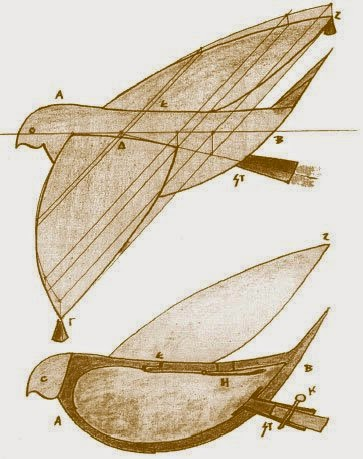
\includegraphics[width=4.1cm,height=5.5cm]{chapters/intro/images/pigionsteam.jpg}}\quad
\end{subfigure}
\begin{subfigure}
[Antikythera mechanism]{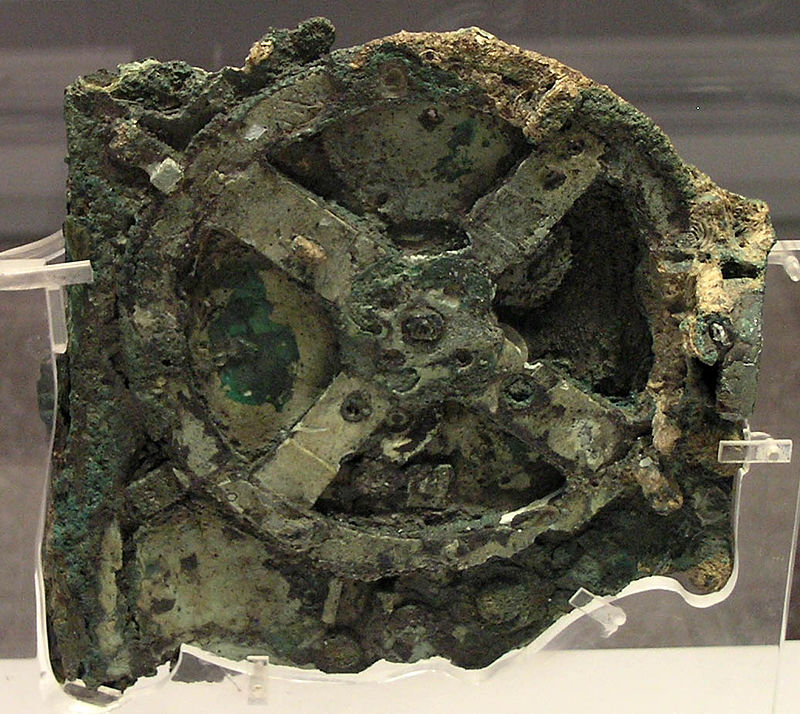
\includegraphics[width=4.3cm,height=5.5cm]{chapters/intro/images/machineanti.jpg}}\quad
\end{subfigure}
\begin{subfigure}
[Su Song's Clock Tower]{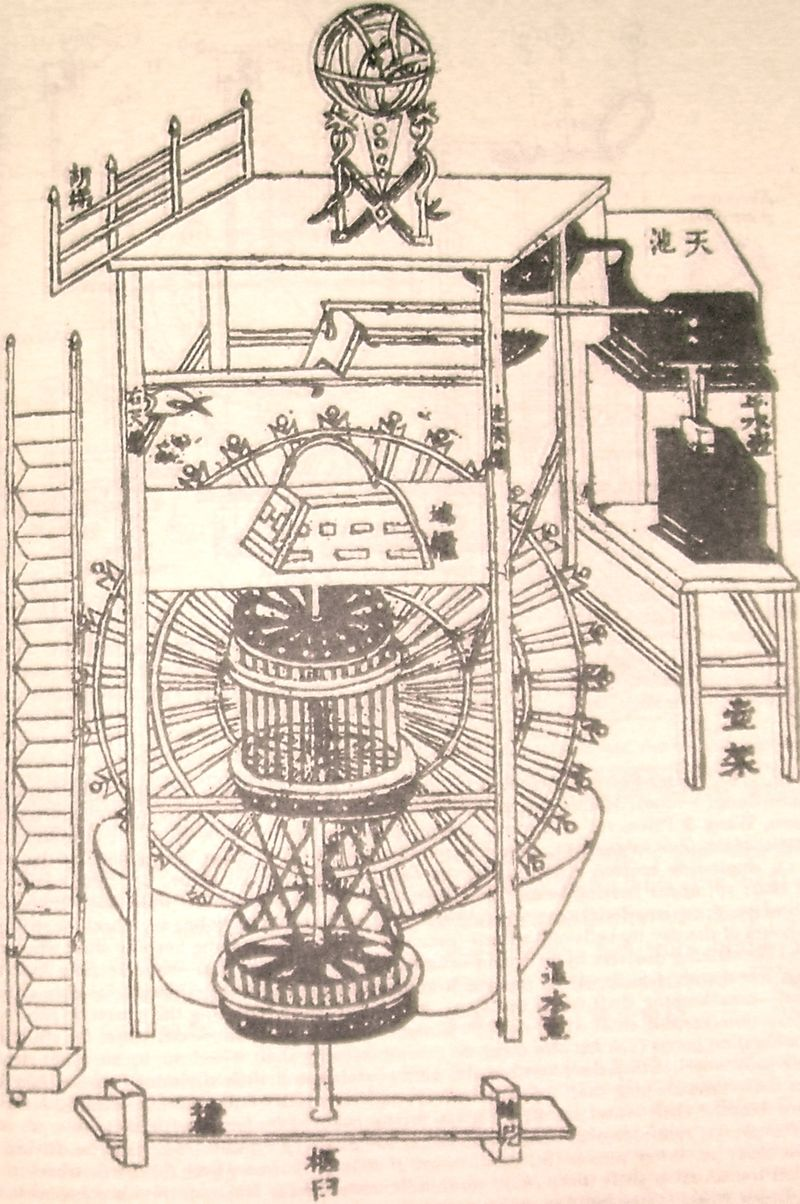
\includegraphics[width=4.1cm,height=5.5cm]{chapters/intro/images/clocktower.JPG}}\quad
\end{subfigure}
\caption{Automatons in the ancient world}
\label{fig:automatons0}
\end{figure*}

Fig.~\ref{fig:automatons1} (a) shows the first ever humanoid robot in the records, designed by Leonardo da Vinci. This mechanical knight has joints similar to human beings with an ability to perform motions such as waving the arms, moving the head and jaws, sitting and standing up. Around 18th century many automatons were developed capable of entertaining, speaking and playing musical instruments. One such musical automaton in the form of an elephant shown in the Fig.~\ref{fig:automatons1} (b) is designed by Hubert Martinet, a french clockmaker in 1774. Another interesting automaton in the Fig.~\ref{fig:automatons1} (c) is the \textit{Digesting Duck} made by Jacques de Vaucanson. This golden mechanical duck imitates the ability to eat and defecate grains.

\begin{figure*}[!tbph]
\begin{subfigure}
[Da Vinci's robot]{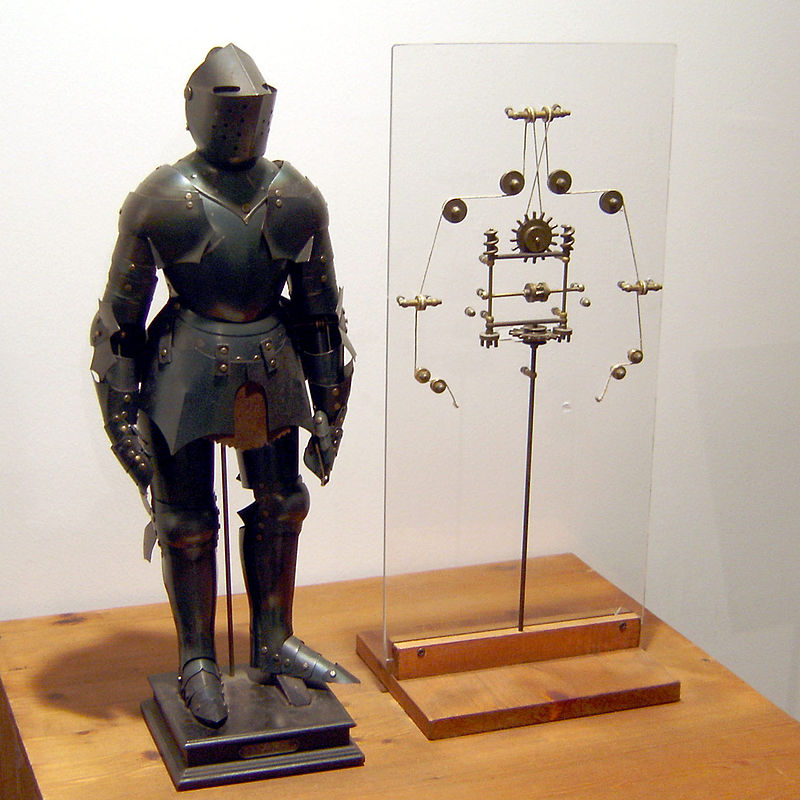
\includegraphics[width=4cm,height=4.5cm]{chapters/intro/images/leorobot.jpg}}\quad
\end{subfigure}
\begin{subfigure}
[Elephant Automaton]{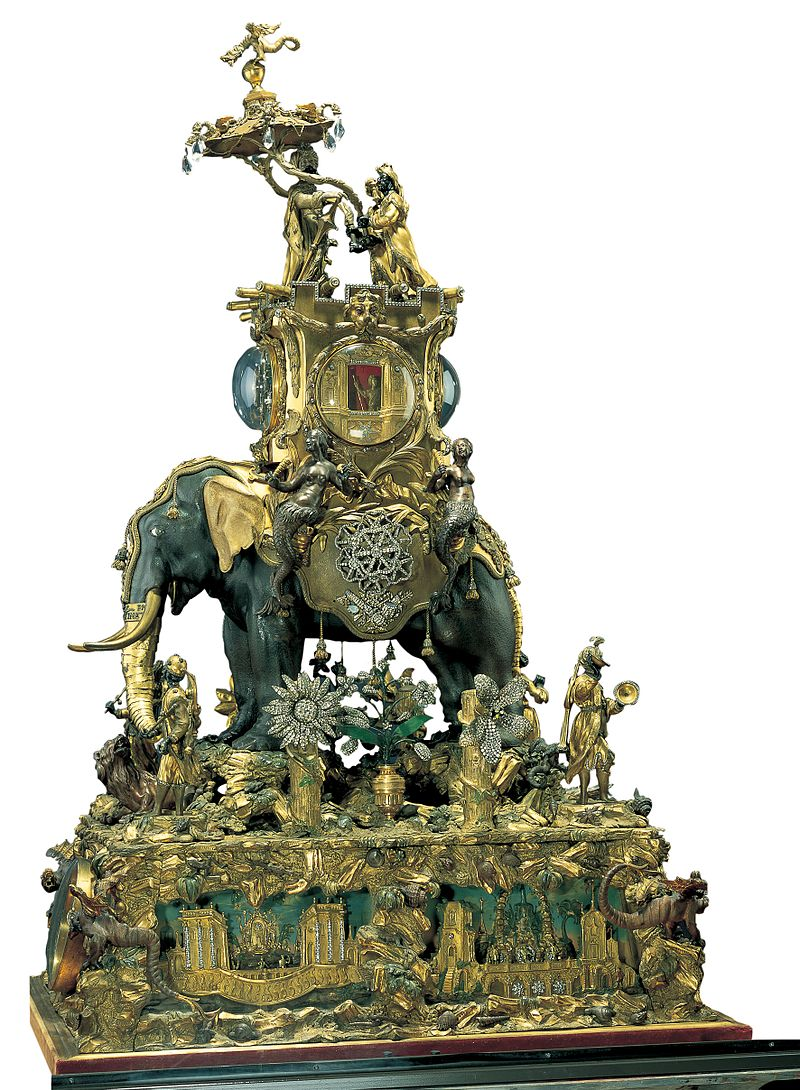
\includegraphics[width=4cm,height=4.5cm]{chapters/intro/images/elephantAutomaton.jpg}}\quad
\end{subfigure}
\begin{subfigure}
[Digesting Duck]{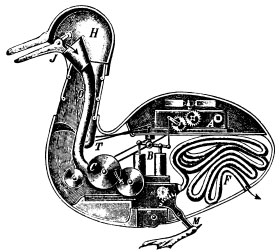
\includegraphics[width=4cm,height=4.5cm]{chapters/intro/images/duck.jpg}}\quad
\end{subfigure}
\caption{Automatons in the 18th Century}
\label{fig:automatons1}
\end{figure*}

% May be talk about Remote-controlled systems

Though most of the automatons were created for fun or artistic satisfaction in the beginning, the characterization of robots to be human look-alike machines that can serve human beings came up in the 20th century. The term \textit{robot} itself was born in 1921 from R.U.R (Rossum's Universal Robots), a czech play written by Karel Čapek. The play depicts robots as good and benevolent workers serving the human beings later gaining super human strength to revolt humans leading to end of life. This negative idea changed after a russian writer, Isaac Asimov made a contrasting characterization of robots as just mechanical creatures with no emotions. Asimov's laws of robotics in 1942 gave way to a new perspective of robots to be seen as an product that could be developed by engineers to improve productivity in manufacturing industries. During the same time period, a programmable mechanism to do spray painting was designed by Pollard and Roselund for DeVilbiss, the first industrial robot supplier. The mechanism is based on pantograph pivoted on two rotary actuators on a fixed base. 


\begin{figure*}[!tbph]
\centering
\begin{subfigure}
[Pollard's Paint Sprayer]{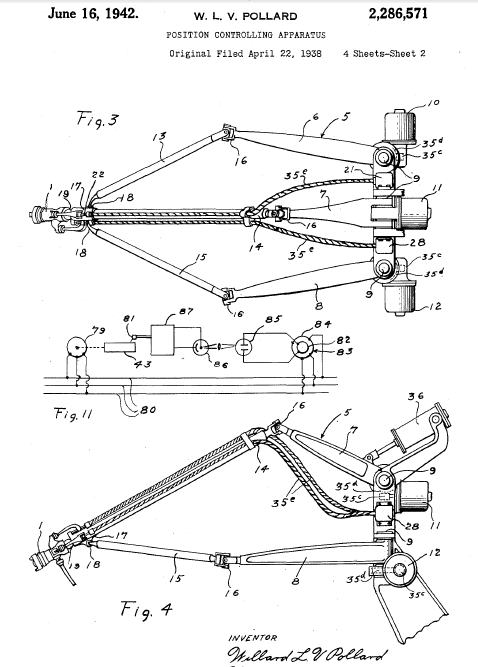
\includegraphics[width=6.5cm,height=6cm]{chapters/intro/images/pollard.png}}
\end{subfigure}
\begin{subfigure}
[Unimate Robot's Television Appearance]{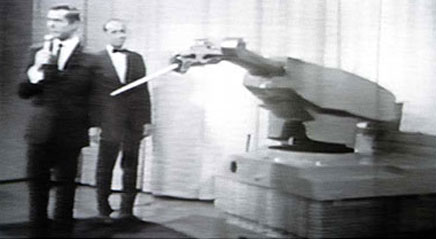
\includegraphics[width=6.5cm,height=6cm]{chapters/intro/images/unimate.jpg}}
\end{subfigure}
\caption{Robotic Mechanisms in the Beginning}
\label{fig:robotmechanisms}
\end{figure*}


In 1954, George Devol developed the the first truly programmable robot UNIMATE which originally consisted of an arm and a drum memory box with pre-programmed tasks. A collaboration with Joseph Engelberger, the father of robotics gave birth to \textit{Unimation}, the first company to make robots which were used to transport and weld die castings on auto bodies preventing humans from dangerous working conditions. Though the numerically controlled turning \& milling machines and the hydraulic assembly machines were programmable, the industrial robots differed in the sophistication of reprogrammability and the versatility to be used for different tasks. This is purely because of the invention of digital computers and integrated circuit technology which allowed to develop the brains of industrial robots.

\begin{figure}[h]
\centering
{\includegraphics[scale=1]{chapters/intro/images/gm.jpg}}
\caption{Manufacturing unit in General Motors with 'Unimate' robots in 1969}
\label{fig:unimate}
\end{figure}

Ford director Del Harder's interest to install 2000 unimation robots triggered American manufacturing industries to pay attention to the robotics industry a bit more seriously. Installations in General Motors in Ohio, US in the beginning of 1960s marks the real beginning of industrial robotics. After an intense research and development during the next 15 years and the introduction of micro-processors provided the basis for low cost control systems. A norwegian company \textit{Trallfa} designed and developed a cost-effective alternative to Unimate robots for spray painting applications. Several companies such as \textit{Electrolux, ESAB, Atlas Copco,} and \textit{ASEA} followed the same path designing in house robots for their own purposes which suited the requirements of other customers resulting in a product of its own. This phenomenon gave birth to more than 70 robot manufacturers by the year 1973.



The industrial robots were hydraulic or pneumatic in the beginning though they are very suitable for heavier loads. Vicarm in 1968 turned out to be the first electric robot to suit the lighter loads of assembly lines and arc welding. The 6 degree of freedom robot (5 revolute + 1 prismatic) was designed with simplified analytic solutions by Victor Scheinman allowing the robot to track arbitrary paths in the work space of the robot. Cincinnati Milacron, the largest machine tool constructor during the 1970s developed the "The Tomorrow Tool", the first microcomputer based robot. The robots in the beginning were used for simple tasks such as pick and place with no external sensing. External sensing along with the ability of robots to perform advanced motion behaviors gave rise to complex applications like welding, grinding and deburring. The applications can be divided to three main categories: Assembly lines, process operations and material handling. The main motivation of industrial robotics is to apply productive, cost-effective and human safe automation solutions without compromising on the quality of the products. 


The capabilities of robots were purely driven by the manufacturing industries with different industries focusing on different requirements. Material handling required robots of increased loading capacity while arc welding and motion dependant applications required the robot to have better electrical motors and path control. In the beginning of 1980s the assembly lines were mostly focused and shorter cycle time has always been the goal which required robots to be highly dynamic and repeatable. Metal industries required the robots to be very stubborn to work in hot and unsafe working environments. Though robots had complex applications, simple applications such as picking and placing, material transportation were economical for automization. 
These customer demands provided way to the industrial robotic revolution in the 1980s. 


\begin{figure}[!tbph]
\begin{subfigure}
[The Tomorrow Tool-T3]{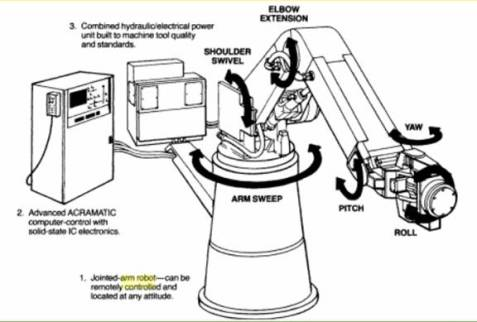
\includegraphics[width=4.3cm,height=6cm]{chapters/intro/images/t3.jpg}}\quad
\end{subfigure}
\begin{subfigure}
[Shakey]{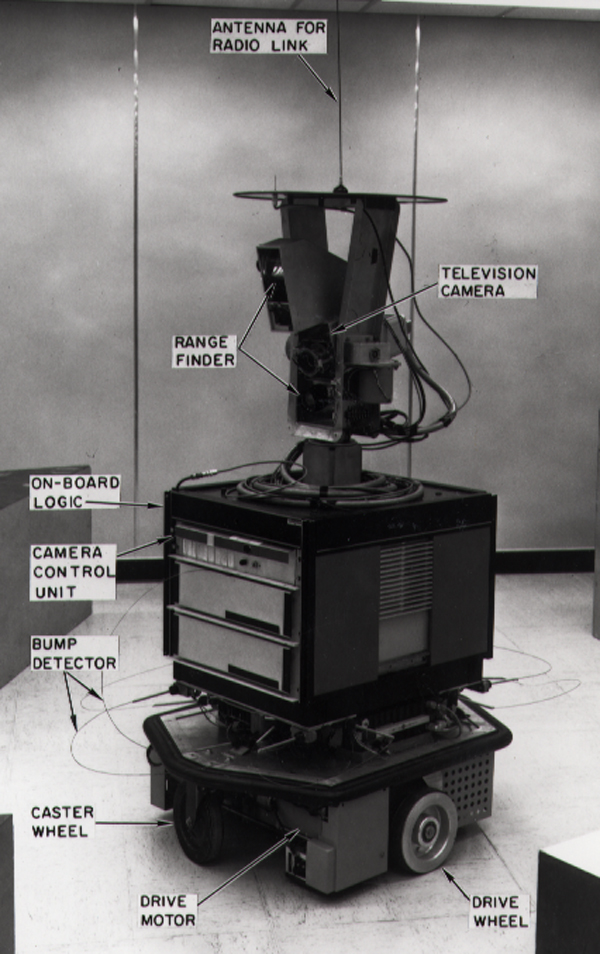
\includegraphics[width=4.1cm,height=6cm]{chapters/intro/images/Shakey.jpg}}\quad
\end{subfigure}
\begin{subfigure}
[Stanford Arm]{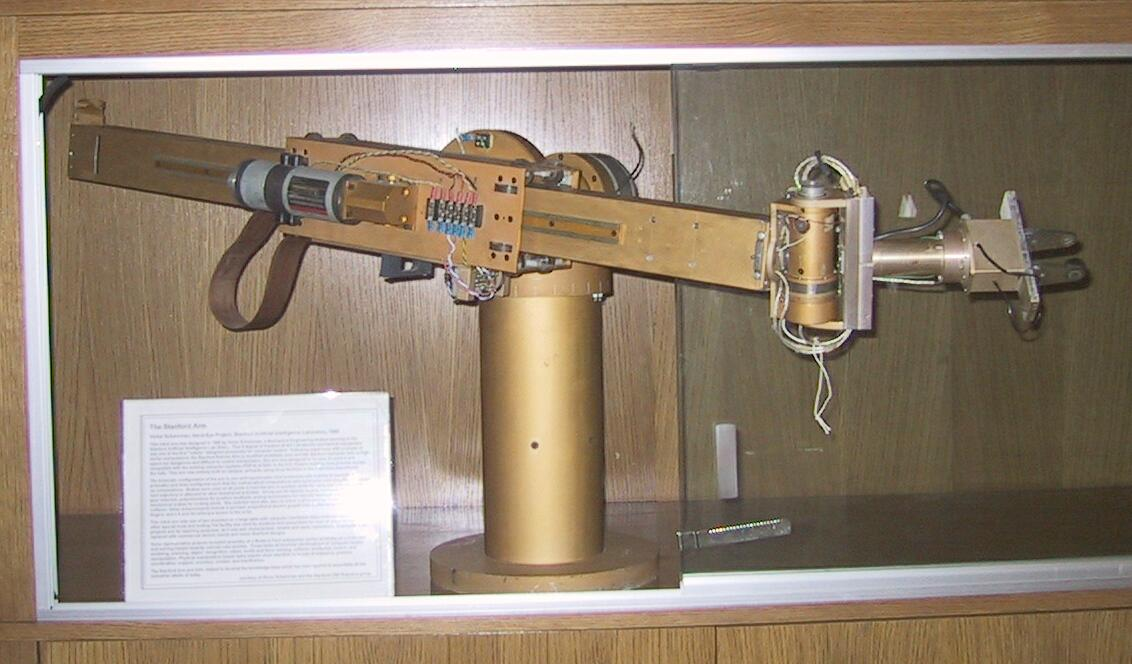
\includegraphics[width=4.1cm,height=6cm]{chapters/intro/images/stanfordarm.JPG}}\quad
\end{subfigure}
\caption{Automatons in the ancient world}
\label{fig:robots}
\end{figure}

Robotics was unanimously accepted as a key focus area to increase industrial development and achieve competitive edge. Advanced sensors such as force sensors, vision cameras and laser scanners were introduced in the late 1980s
to make physical interactions with the environment to improve the intelligence. It is necessary to make deeper connections with the control system to make intelligent decisions in the working environment. Though the vision of robotics in the 1980s was very ambitious to automise factories completely with robots and less human labour, it was very soon realized that robotics being a multi-disciplinary technology is not so easy and certain human work mechanisms are difficult to be replicated. Heterogenous integration of complex systems involves a lot of problems and developing a robotic workcells are more expensive than the workers themselves though they are economically feasible for simpler tasks.

Productivity is a complex concept and the idea of robots solely responsible for improving productivity changed in the beginning of 1990s. The dependence on robotics for more ambitious tasks started to decrease though it was and still an inevitable part of the mechatronic technology to automize and improve productivity. Now robotics are used for medical applications, service, entertainment and disaster handling applications. Though the industrial robots have been in use for quite a long time, there are many challenges not addressed until now. This is where the 'Factory in a Day' project comes into picture.

\subsection{'Factory in a Day' project}
We are aware that robot automation has been into existence since the 1960s and has seen a lot of technological advancements but they are still challenged by installation time and cost involved in setting up robots specific to the functional needs in factories. There is a lot of risk involved in such investment making it economically less attractive to smaller companies. Moreover, the factory setups are fixed environments with hard coded settings of millimeter precision so that they are perfectly under control at all times. Floating robot bases introduces errors and uncertainties which requires more robust components to handle factory scenarios. There is also a big concern in safety of human beings working in robot environments. Though recent technologies are focused towards collaborative robot control where human beings and robots can work together, these algorithms are either completely not matured to be used in factories or not yet known in the industrial community. This thesis is funded by Factory-in-a-Day project which focuses on these issues mentioned above.

Factory-in-a-Day project puts forward the idea of minimizing the installation time and the cost involved from several months to just a single day. The project focuses on the following aspects of robotics which is synonymous to the steps taken in a day to install a robotic setup. 

\begin{itemize}
\item Standardized procedures to design 3D printed custom parts which are usually attached with an existing robot arm and grippers using novel templates to minimize the time taken.
\item The flexibility to be placed in factories without any alteration where intelligent self-calibration and an adaptive framework that helps to connect with the existing machineries in ease.
\item Use rapid teaching to program production tasks in the setup from a rich set of learnable skills
for applications like mould finishing, welding and assembly.
\item Visually intuitive tools for the workers in the factory to assess robot's behavior motion behaviors. Augmented reality can be used to visualize the robot's intended path by wearing a glass to be aware of its activity to be collaborative in nature.
\item A mature human-robot interaction framework to allow the humans collaborate with robots in an unfenced workspace using a dynamic obstacle avoidance framework with proximity skin sensors and 
reactive path planning and control algorithms.
\end{itemize}
The above aspects along with proposed certification procedures and a complete focus on manufacturing industry can radically change the automation sector. The work done in this thesis orients in the direction of the last aspect which is human-robot collaboration. The Fig.~\ref{fig:doa_motivation} (a) shows the reality of many robotics based manufacturing units with fences avoiding dangerous accidents with human beings. There are strict protocols followed to get inside the fence incase of repairs needed. It is definitely not productive, and the new age robot manufacturers such as \textit{Universal Robots} focus on manufacturing robots with safe touch control which allows the robot to stop when the human is in contact. In case the robots are moving fast, they can be programmed to adapt/reduce the speed by monitoring the presence of human beings using laser scanners. Though there are systematic hacks available, the thesis supports the idea of human-robot collaboration in the real sense where they share the workspace with more awareness about the environment and task scenarios. 
\begin{figure}[!tbph]
\begin{subfigure}
[Fenced Robot for Safety]{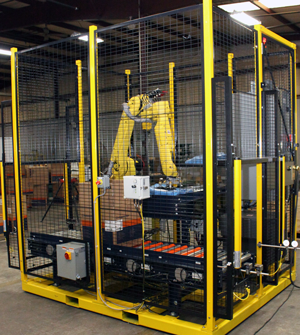
\includegraphics[width=6.6cm,height=6cm]{chapters/intro/images/fencedrobot.png}}\quad
\end{subfigure}
\begin{subfigure}
[New Gen Universal Robot]{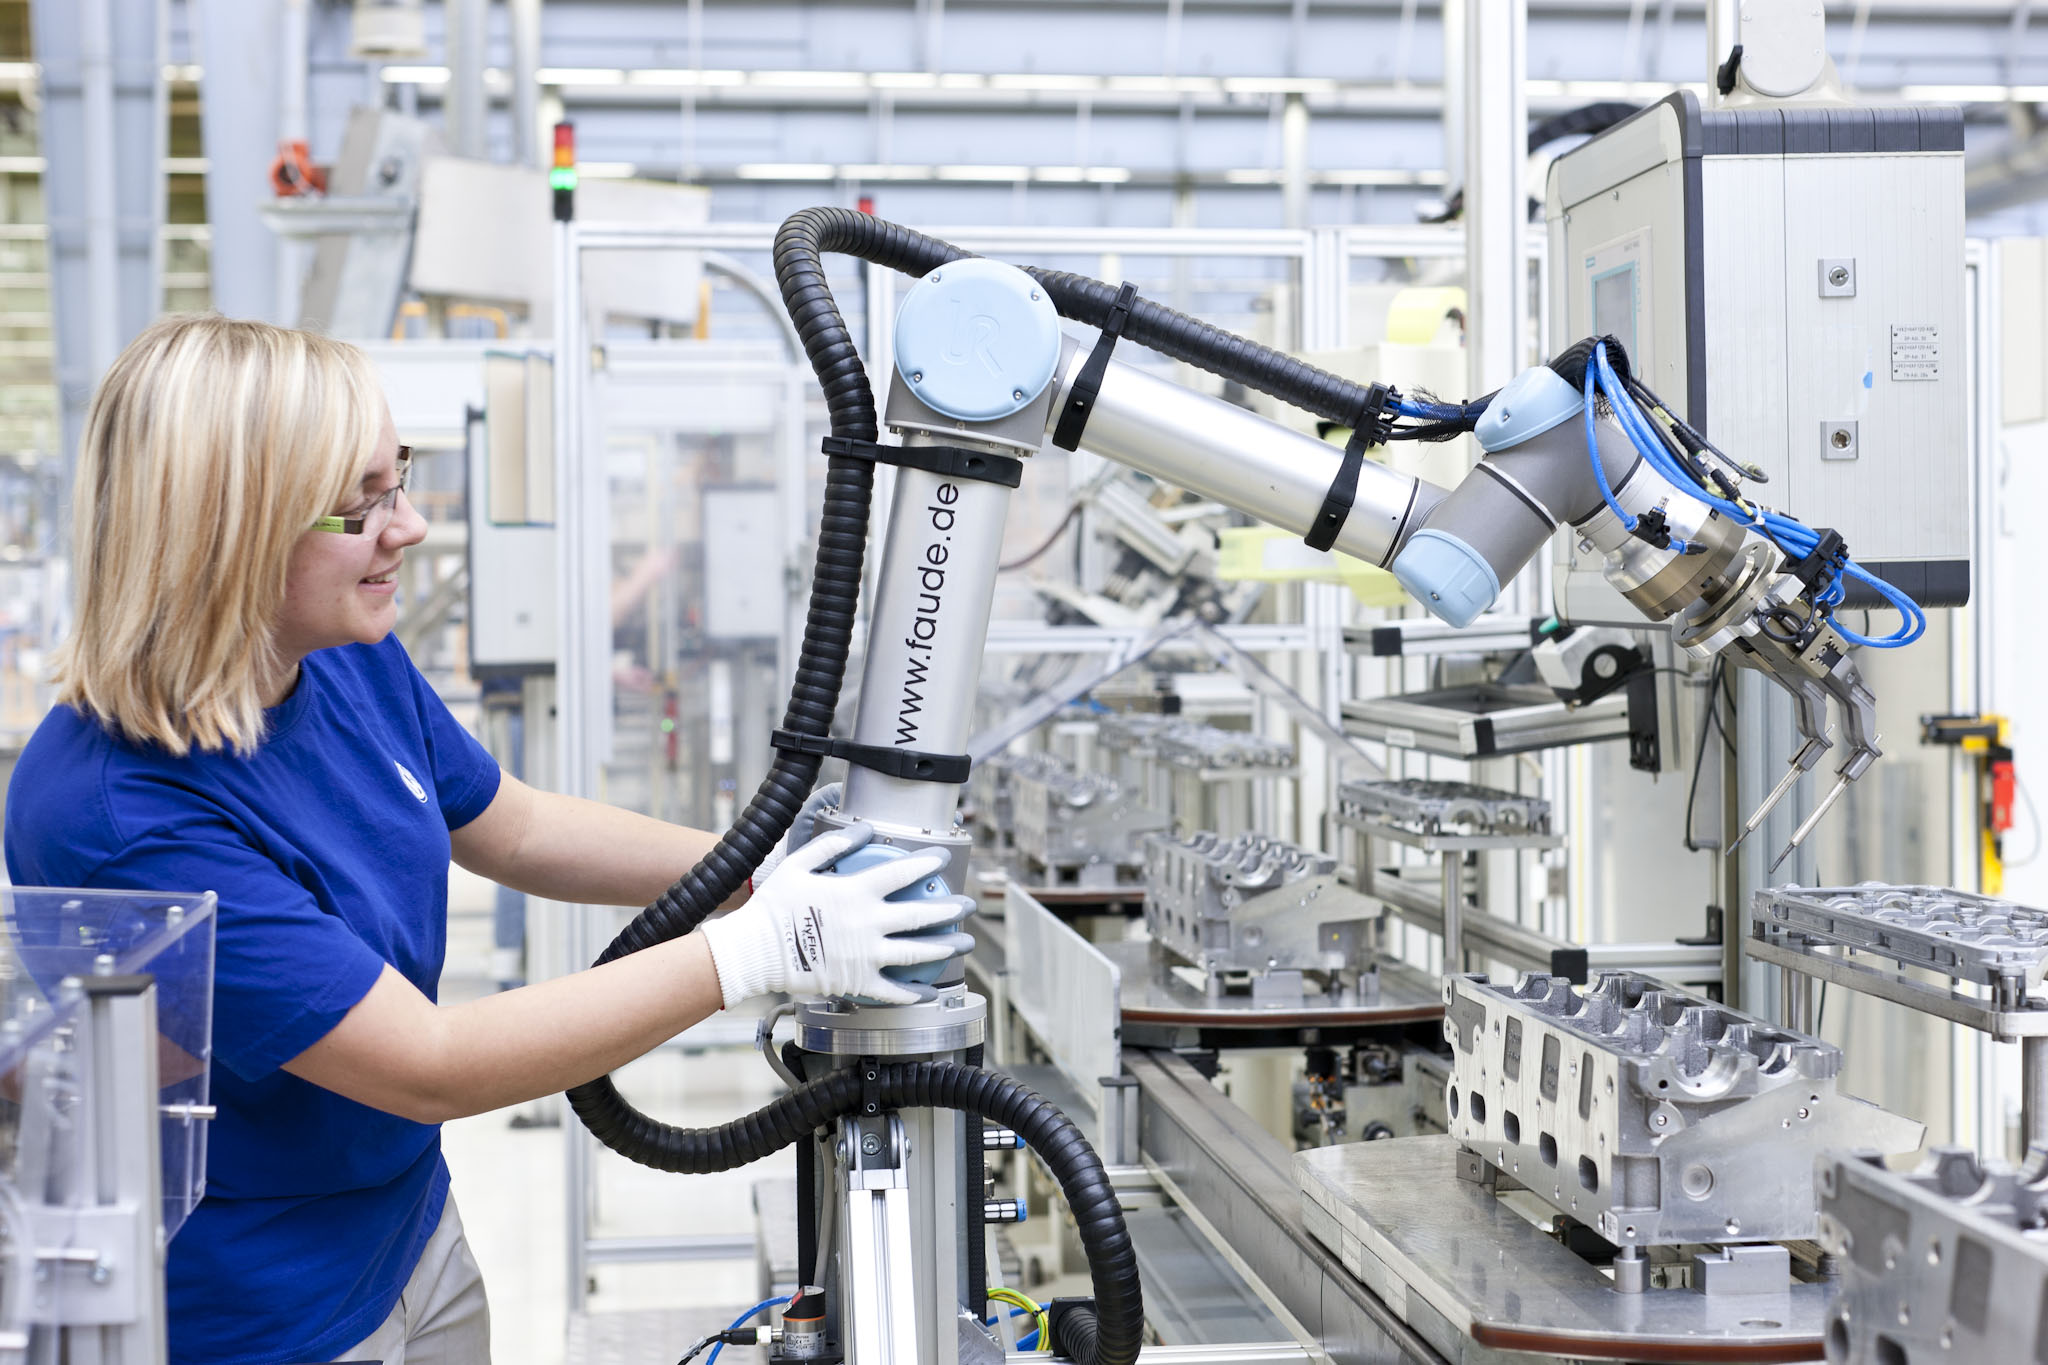
\includegraphics[width=6.5cm,height=6cm]{chapters/intro/images/urcorobot.jpg}}\quad
\end{subfigure}
\caption{Motivation towards Collaborative Robots}
\label{fig:doa_motivation}
\end{figure}


\section{Humanoid Robots}
Humanoid Robots are robotic mechanisms resembling the kinematics of human beings with a head and a torso bridging two arms \& two legs. There are many variants modeling only certain parts of the human body though we stick with the context of legged robots with arms through out this report. Building humanoid robots require the need of understanding human behaviors and kinematic structure deeply. Attempting to build such robots sometimes give us better understanding of human beings making the knowledge flow between both the domains bi-directional. The anthropomorphic design of humanoids also help in getting the acceptance of people as a social entity making the human-robot interaction feasible \cite{fink2012anthropomorphism}. Also the physical ability of humanoids make them suitable for rescue or disaster handling scenarios. The social acceptance and the physical ability of humanoids make them a very good platform to invest on researching technologies that improve the intelligence of such robots.

\subsection{History of Humanoid Robots}
Humanoid robots were just controlled using traditional joint position control methodologies like in industrial robots though there is a need for stiff drive train for precision. WABOT-1 was the first humanoid robot to walk, communicate, visually recognize objects and manipulate them. The robot was built by Kato's lab from University of Waseda in 1973 \cite{kato1973development}. The same lab lead a series of developments achieving the latest one WABIAN-2 which can walk with stretched knees \cite{ogura2006development}. Chronologically WABOT-1 was followed by P2, the first robot to perform stable walking, was launched in 1996 by Honda after 10 years of modular and systematic research focused on dynamic biped walking and stability control \cite{hirai1998development}. The next version P3  was much lighter and gave way to the launch of the famous ASIMO robot in 2000 with a more friendly appearance and improved intelligence \cite{hirose2007honda}. ASIMO's impressive capabilities attracted the attention of robotics researchers and created a perspective of humanoid robots to be exploited for service robotics \cite{kaneko2009cybernetic}. 


\begin{figure}[!tbph]
\begin{subfigure}
[WABOT-1]{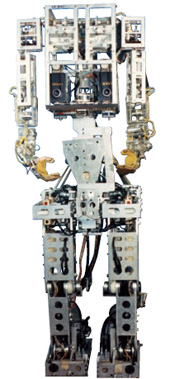
\includegraphics[width=4.1cm,height=6cm]{chapters/intro/images/wabot1.jpg}}\quad
\end{subfigure}
\begin{subfigure}
[ASIMO]{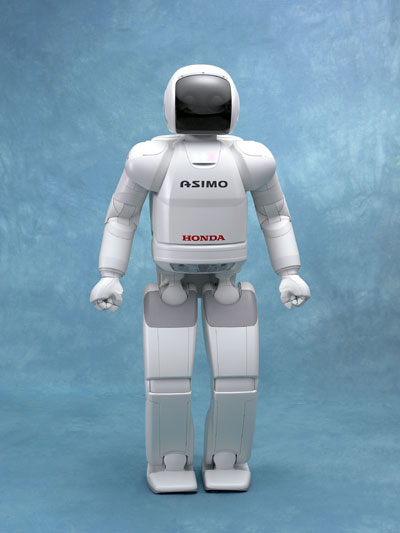
\includegraphics[width=4.2cm,height=6cm]{chapters/intro/images/asimo.jpg}}\quad
\end{subfigure}
\begin{subfigure}
[Kobian]{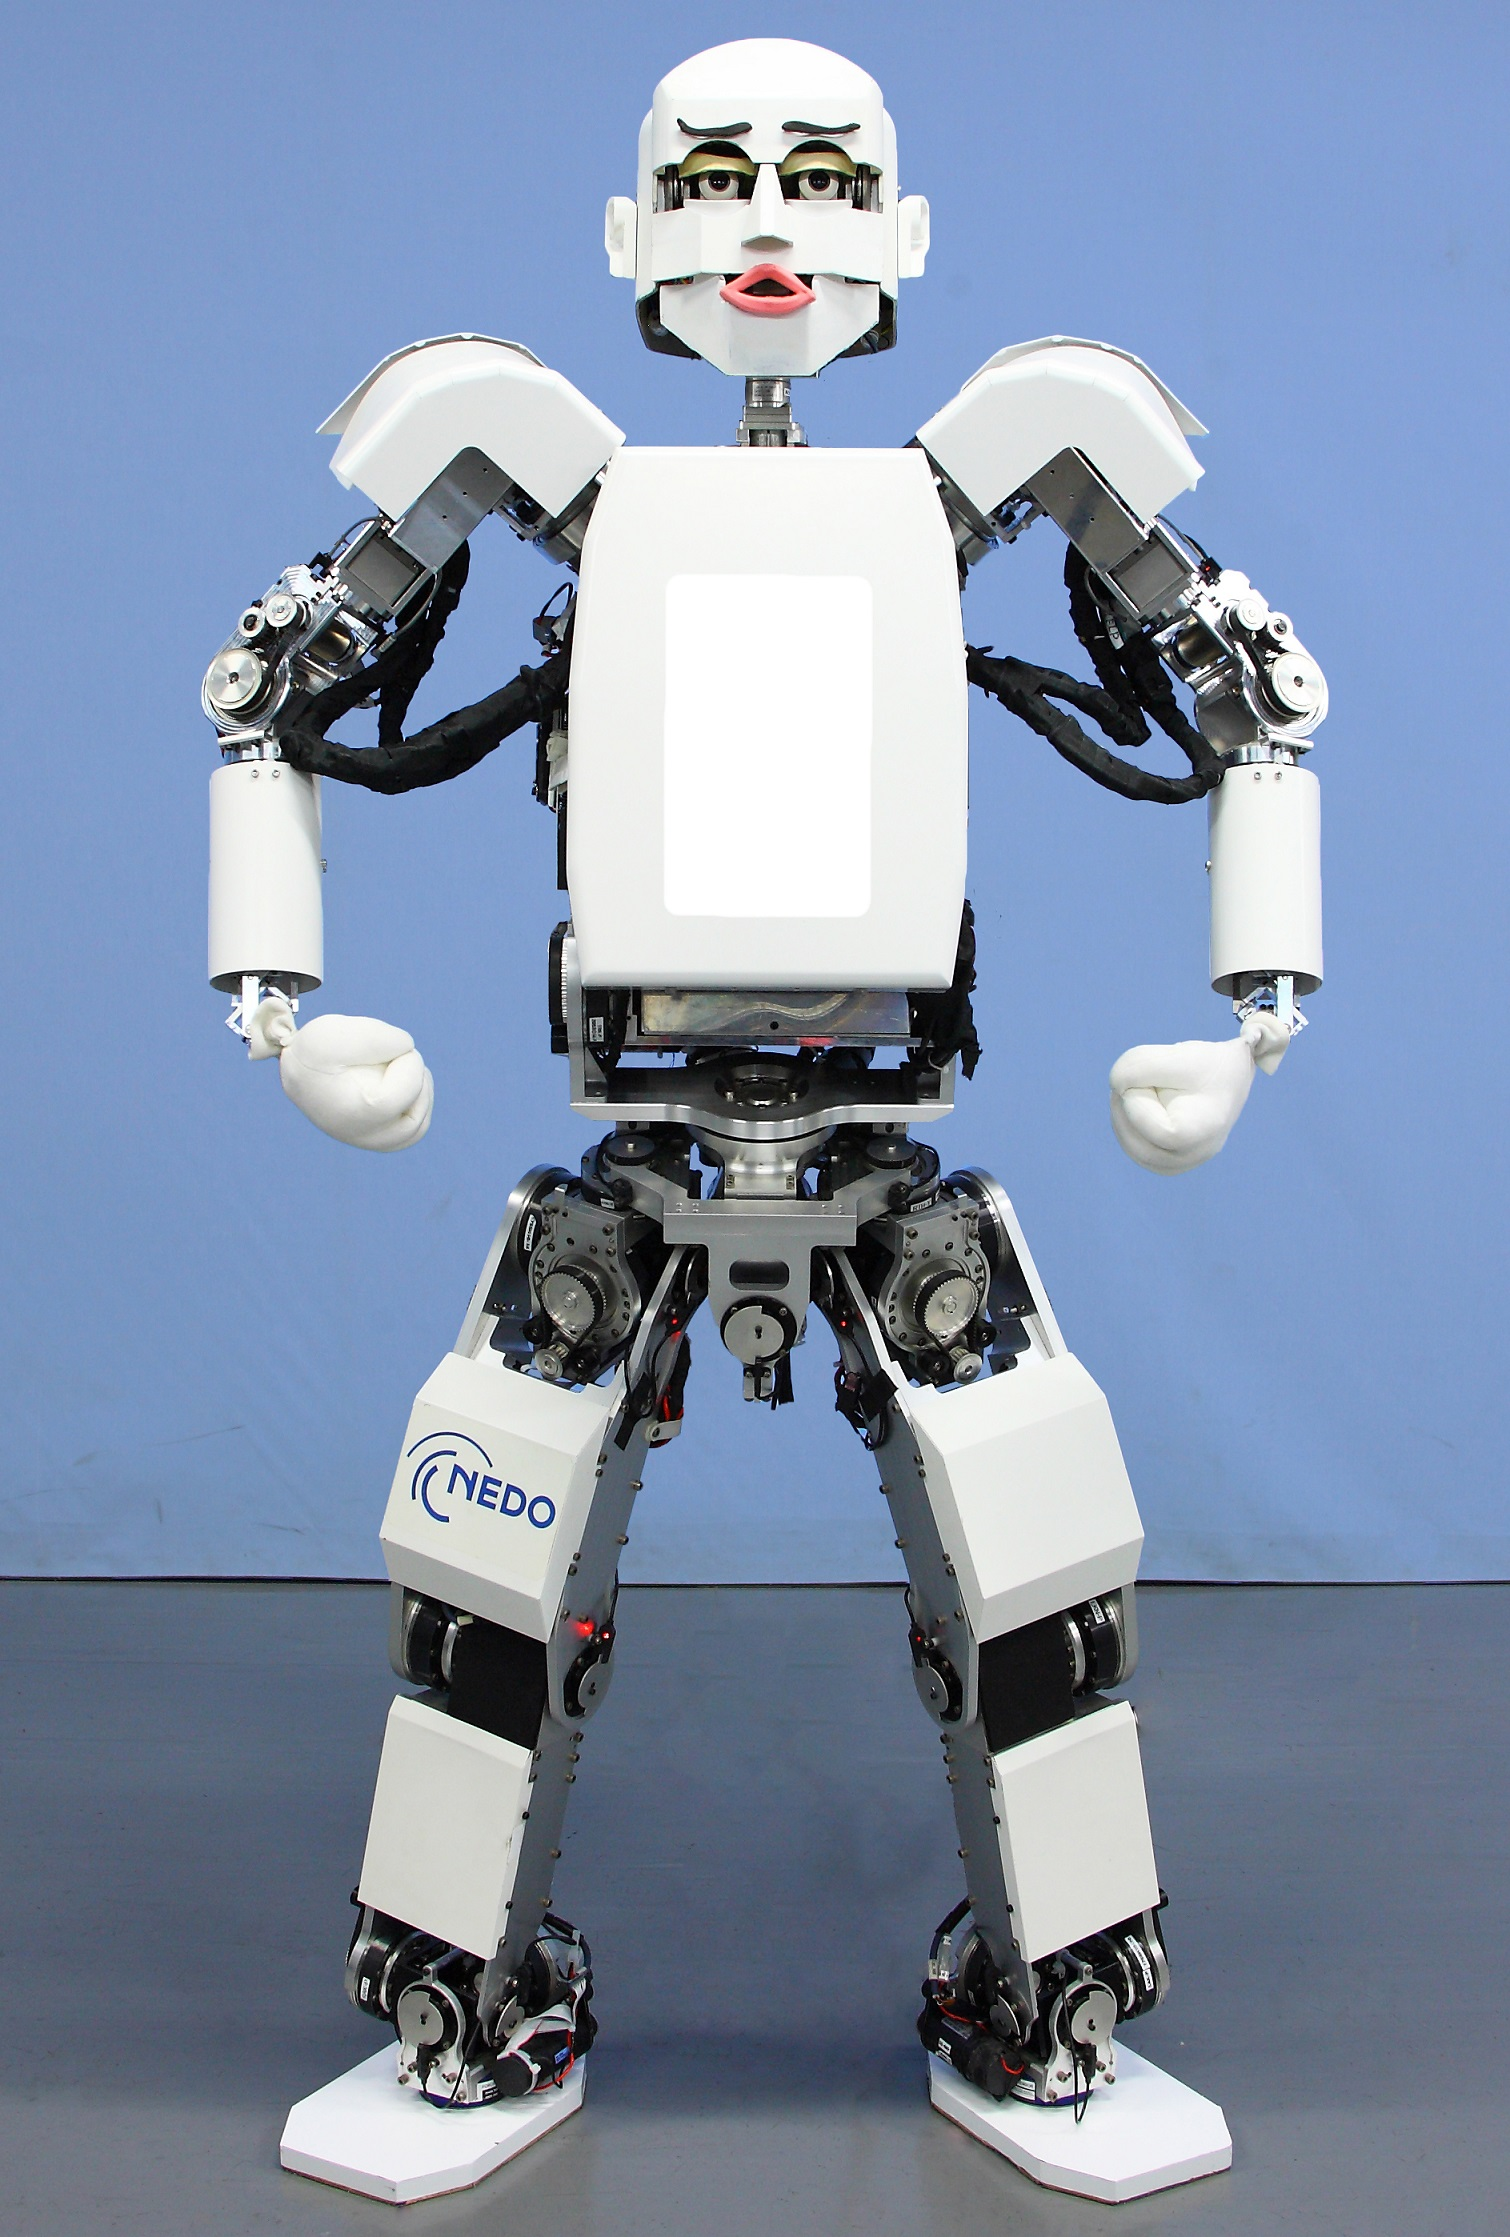
\includegraphics[width=4.2cm,height=6cm]{chapters/intro/images/kobian.jpg}}\quad
\end{subfigure}
\caption{Humanoids of the first generation}
\label{fig:hr_first}
\end{figure}


Japan took the trigger seriously and many humanoids were developed in the last decade both for entertainment and demonstrating physical capabilities. Different sized humanoids with great capabilities were built within the \textit{Humanoid Robotics Project} by Kawada Industries and Japanese National Institute of Advanced Industrial Science and Technology (AIST)  with the first prototype HRP-2P launched in 2002 \cite{kaneko2002design} followed by HRP-2 \cite{Kaneko04humanoidrobot}, HRP-3 \cite{kaneko2008humanoid} in the next years. HRP-4C in 2009 \cite{kaneko2009cybernetic}, assumes a feminine appearance while the latest HRP4 in 2010, is more athletic and light \cite{kaneko2011humanoid}. Sony launched QRIO (previously called SDR-3X), a small humanoid robot for entertainment in 2004 \cite{geppert2004qrio}. Fujitsu Automation also launched a series of small humanoid robots HOAP with the latest version HOAP-3 released in 2005. Other japanese robots include H7  from the University of Tokyo \cite{nishiwaki2007experimental}, Kenta, a musculo-skeletal robot \cite{inaba2003building}, Kojiro in 2007 \cite{mizuuchi2007advanced},Kenshiro in 2012 \cite{nakanishi2012design}. Schaft launched one of the most powerful humanoid robots inspired from HRP-2 series robots in 2013.

The Korea Advanced Institute of Science and Technology (KAIST) invested in developing several versions of KAIST humanoid robots(KHR) since 2002 with the latest one released in 2011 with the name HUBO 2 \cite{kim2002development,park2005mechanical,park2005development,grey2013multi}. The other well known network based robots from Korea are the MAHRU and AHRA series \cite{you2005network,kwon2007biped, kim2011providing}. Technical Unversity of Munich (TUM) built the humanoid robot Johnnie \cite{gienger1999design} followed by an improved version called Lola \cite{lohmeier2009humanoid} known for its fast and robust motions. The Italian Institute of Technology (IIT)  built a torque controlled iCub \cite{metta2010icub} and COMAN in 2012
\cite{tsagarakis2013compliant}. The University Carlos III from Spain, built the Rh-1 in 2007 \cite{arbulu2007real} and its successor TEO in 2011 \cite{monje2011full}. Pal Robotics also built the humanoid robots REEM-B \cite{tellez2008reem}, REEM-C, a human friendly design in 2014 \cite{robotics2014reem}. In 2007, Aldebaran Robotics, a french company launched Nao, one of the most popular small humanoid robot in the world motivated several laboratories to do research on humanoids with less investment \cite{gouaillier2009mechatronic}. The same company presented a torque controlled child-size robot Romeo. 

\begin{figure}[h]
\begin{subfigure}
[HRP2]{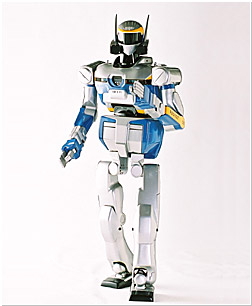
\includegraphics[width=4.4cm,height=6cm]{chapters/intro/images/hrp2.jpg}}\quad
\end{subfigure}
\begin{subfigure}
[Kojiro]{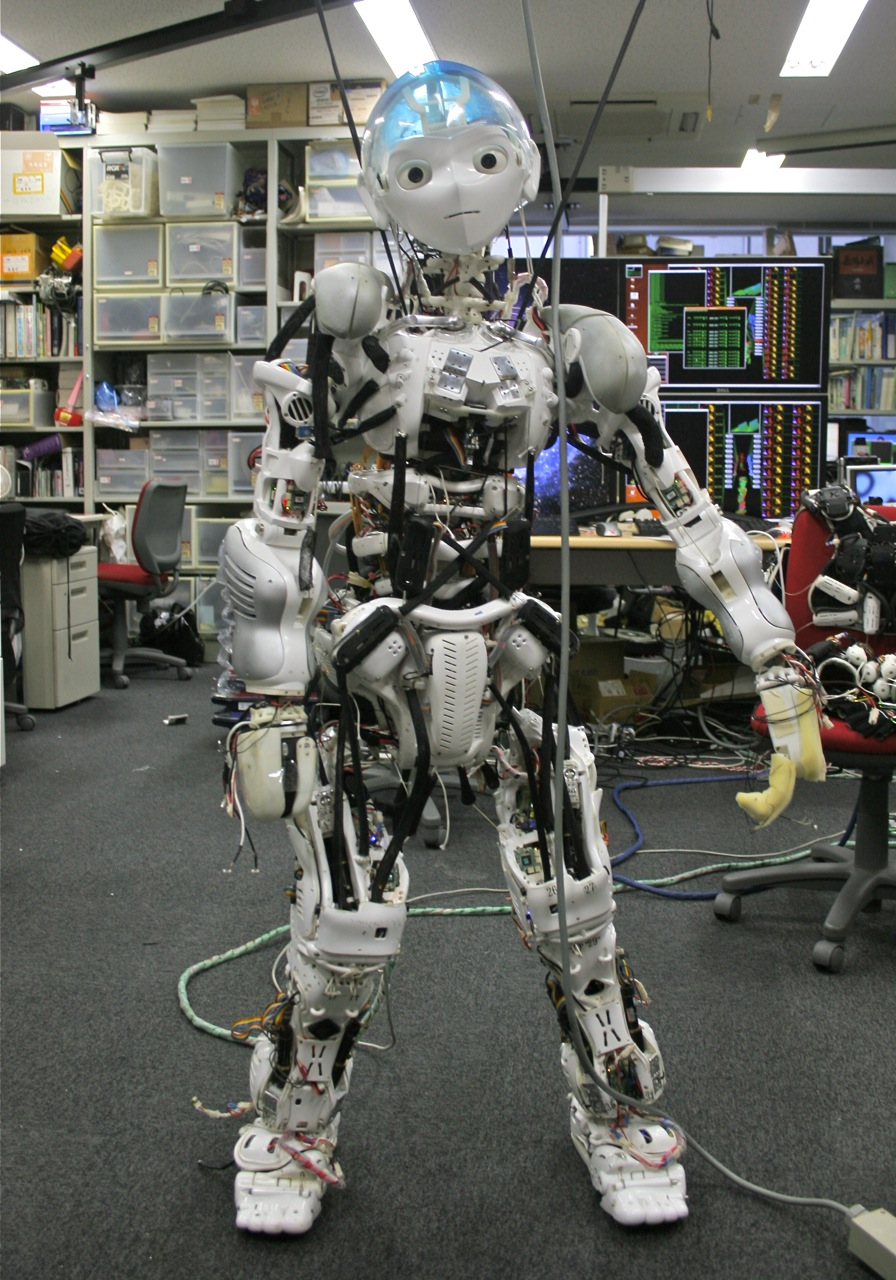
\includegraphics[width=4cm,height=6cm]{chapters/intro/images/kojiro.jpg}}\quad
\end{subfigure}
\begin{subfigure}
[Kenshiro]{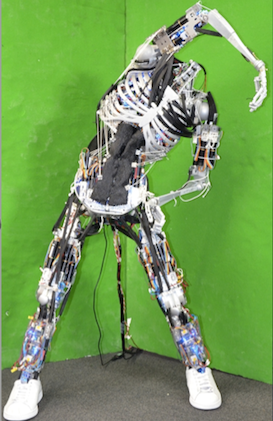
\includegraphics[width=4.1cm,height=6cm]{chapters/intro/images/kenshiro.png}}\quad
\end{subfigure}
\caption{Japanese Humanoids }
\label{fig:hr_second}
\end{figure}

SARCOS Research Corporation and ATR (Advanced Telecommunications Research Institute International) from Japan built robots Erato DB (Dynamic Brain) based on hydraulic actuation in 2000 \cite{atkeson2000using}, and CBi in 2006 \cite{cheng2007cb} which explores the background neural processes in the human brain. DARPA Robotics Challenge (DRC), a competition funded by US Defense Advanced Research Projects Agency (DARPA)  was held between 2012-2015 motivated the development of humanoid robots in the US.  CHARLI in 2010 \cite{knabe2013team}, THOR in 2014 \cite{yi2015team}, CHIMP in 2013 \cite{stentz2015chimp}, Valkyrie in 2013 \cite{radford2015valkyrie} are some popular robots in the US.Most of the robots presented above are fully actuated electrical systems which usually compose rigid bodies with compliance only in the foot to handle contact impacts from the ground while walking. Also they mostly use the traditional high-gain position control methodologies which requires a precise robot dynamic model and Zero Moment Point (ZMP) concept by Vukobratovic \cite{vukobratovic1972stability} is applied in the control of many bipeds \cite{hirai1998development,Kaneko04humanoidrobot,grey2013multi}. 

The advanced robots are expected to make intelligent interactions with the environment. Torque control has gained enough attention in the recent past for its ability to make robust and compliant interactions with the environment and human beings with greater agility and safety. Human safety is one crucial issue which doesn't allow service robots in mobile or humanoid form to be commercialized as domestic robots. Higher compliance brings automatic adaption to un-modeled and uncertain environments making the interaction safer than executing the traditional position control on robots. There are two main categories of torque control: Impedance control and Inverse dynamics control. Impedance Control \cite{part1985impedance,albu2007unified,ott2008passivity,schaffer2008soft} is known for its passivity properties very suitable for interaction with humans and unknown environments. Inverse dynamics(ID) control \cite{del2016implementing,buchli2009compliant,righetti2013optimal} is a highly complex technique which needs a dynamic model and joint torque measurements to control the interactions with the world. This technique provides good trajectory tracking and highly compliant behavior with low feedback gains. The new age ID controllers use quadratic programming(QP) solvers which allow to add constraints such as joint limits, torque bounds, contact force friction cones,center of pressure (CoP) limits which are crucial in humanoid robots. The interest in torque control of humanoid robots lead to new range of robots with torque sensing though it can be estimated in robots with no torques sensors as in HRP-2, iCub, HRP-4 and Asimo, etc.
\begin{figure}[!tbph]
\centering
\begin{subfigure}
[SARCOS]{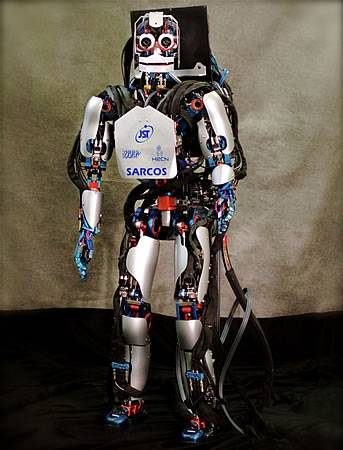
\includegraphics[width=4.2cm,height=6cm]{chapters/intro/images/sarcos.jpg}}\quad
\end{subfigure}
\begin{subfigure}
[CHIMP]{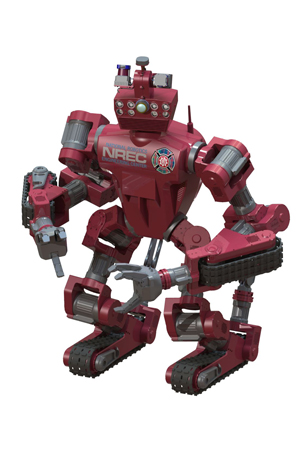
\includegraphics[width=4.2cm,height=6cm]{chapters/intro/images/chimp.jpg}}\quad
\end{subfigure}
\begin{subfigure}
[Valkyrie]{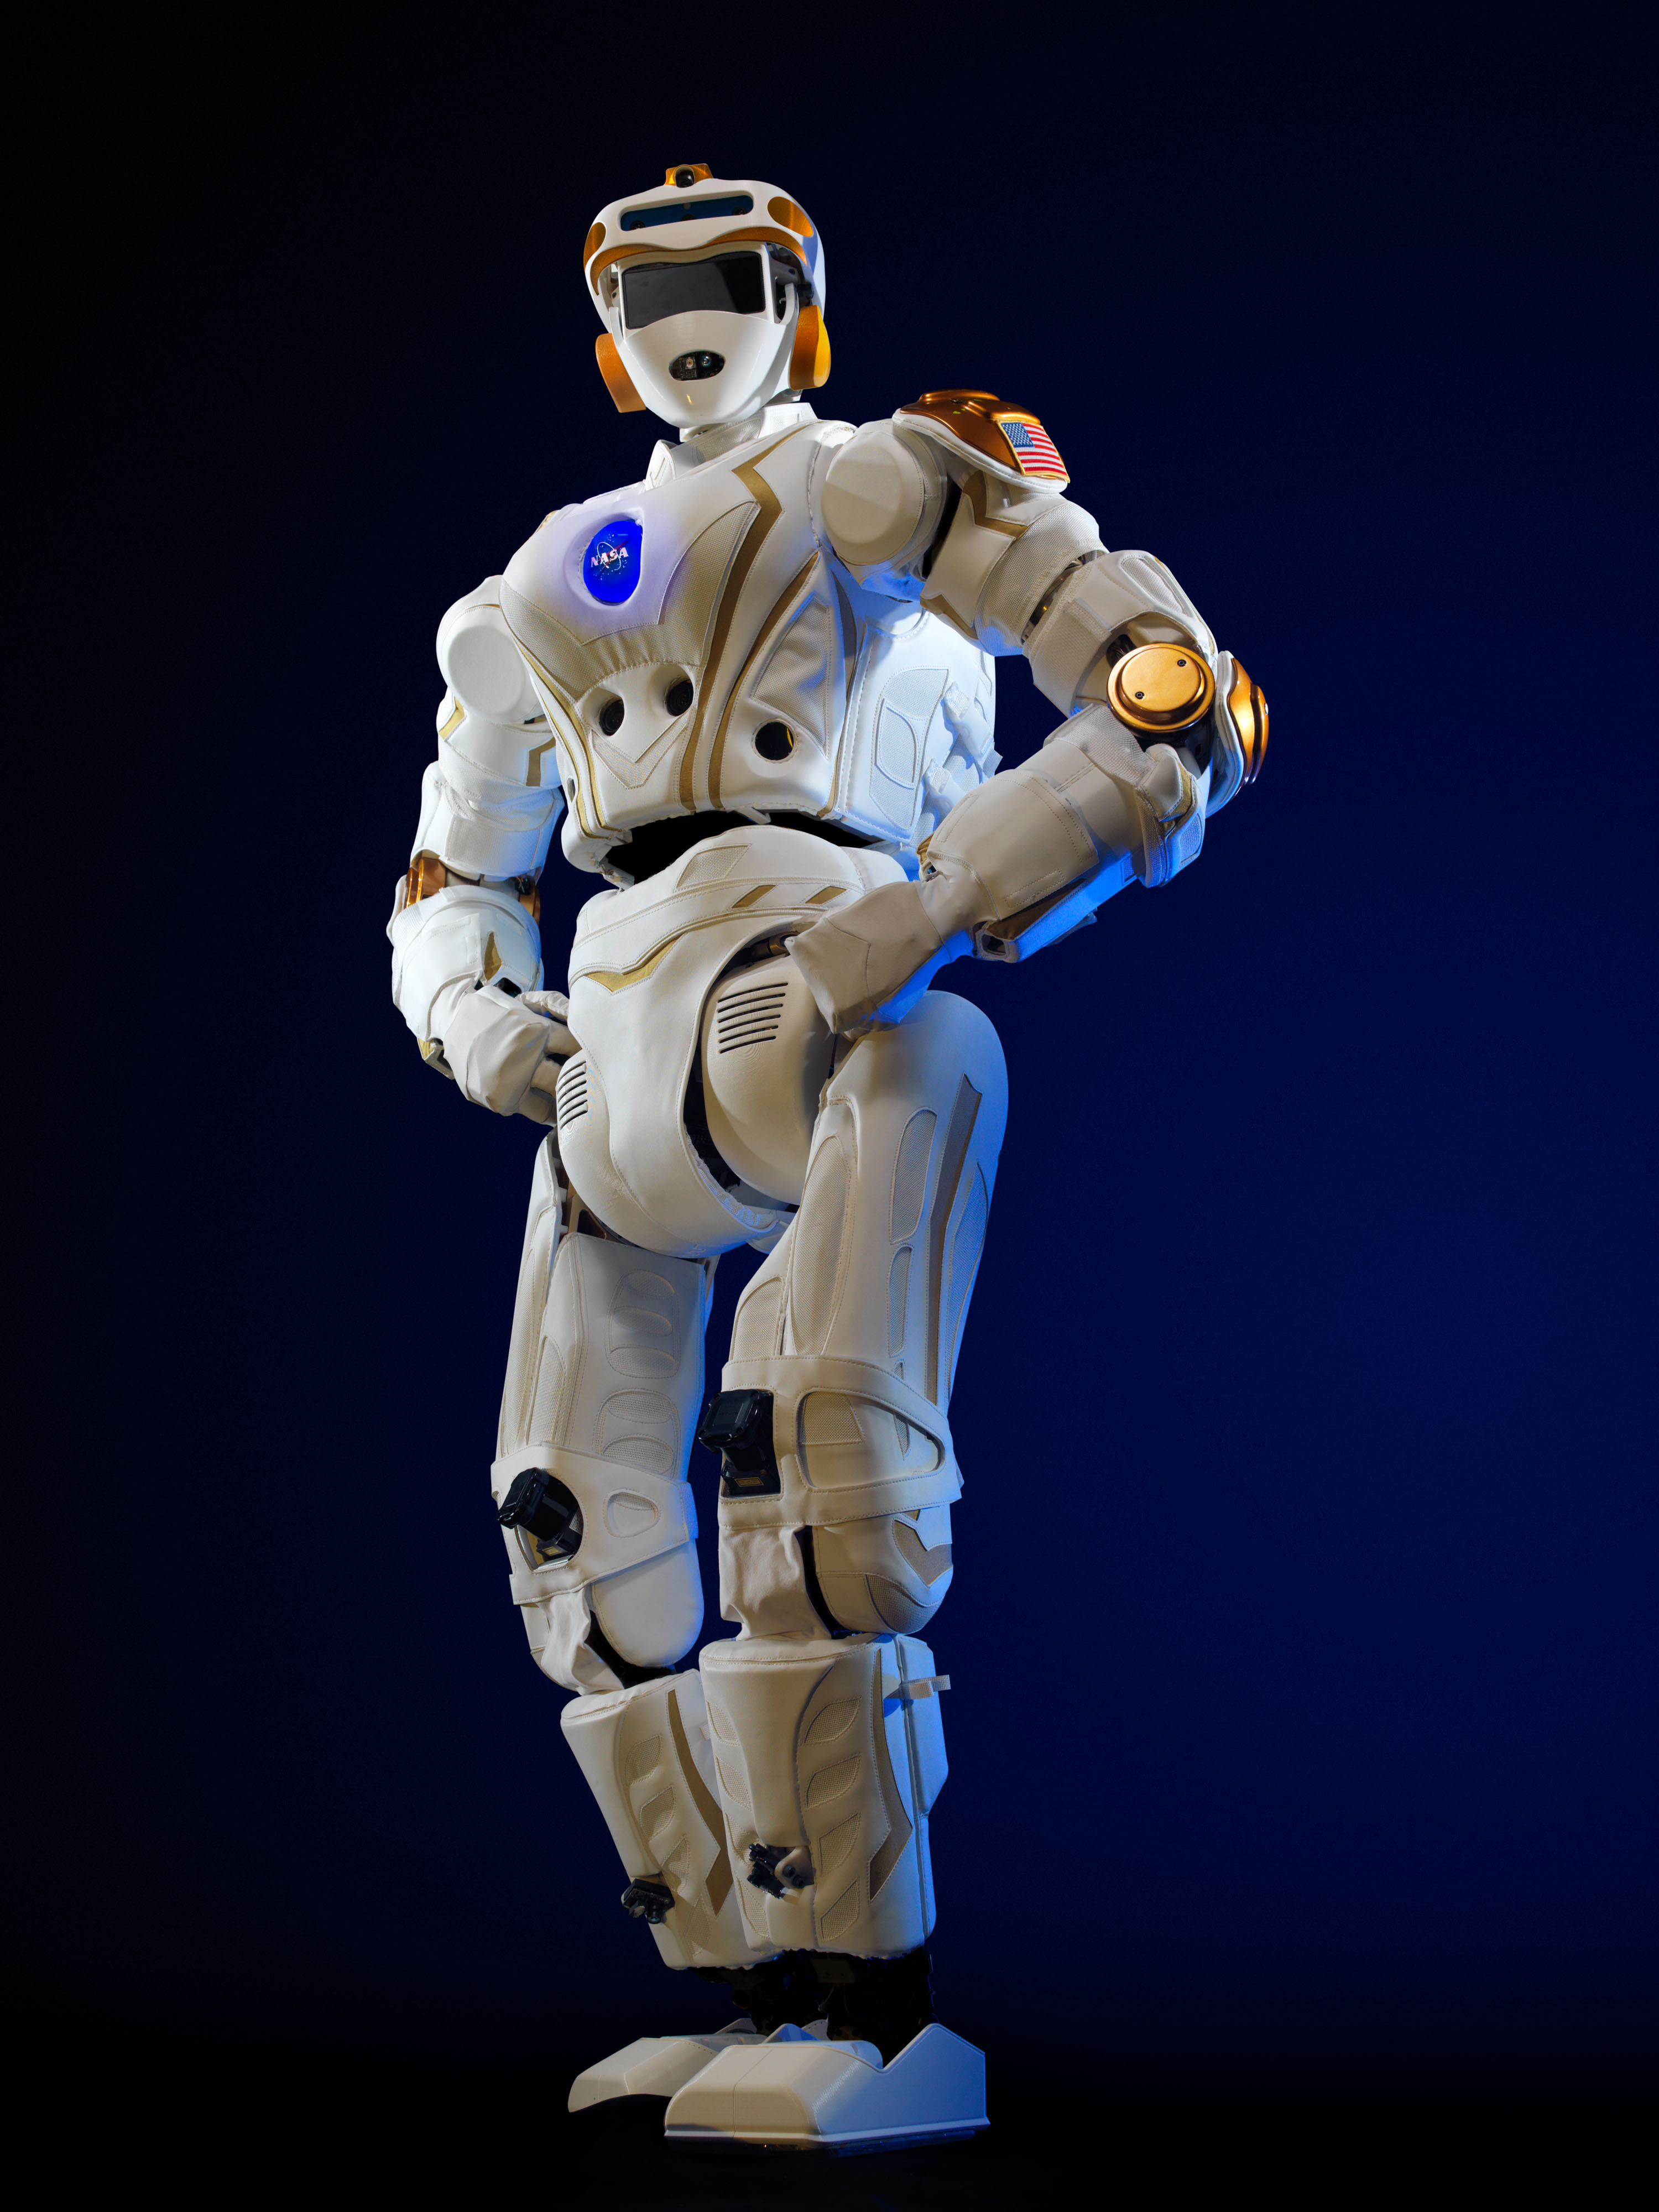
\includegraphics[width=4.2cm,height=6cm]{chapters/intro/images/valkyrie.jpg}}\quad
\end{subfigure}
\caption{Advanced Humanoid Robots}
\label{fig:hr_second}
\end{figure}

 Boston Dynamics built the hydraulics based Petman \cite{nelson2012petman} in 2012 and a series of Atlas robots from 2013. The demonstration video of Atlas in 2016 illustrated the powerful capability of the hydraulic robots by performing tasks which were impossible in the robots of the previous generation. Hydraulic actuation provides high bandwidth and high power density with the price of huge power requirements and noisy hydraulic pumps. High un-modeled friction/stiction makes it harder to control and also the high strength of actuators doesn't allow safe human-robot interaction. Series elastic actuators are also used by some laboratories in their humanoid platforms to implement torque control. The deflections in spring are measured to sense torque, and regulated to execute control on the robot. StarlETH from ETH \cite{hutter2012starleth}, IIT’s COMAN robot \cite{tsagarakis2013compliant}, Human Centered Robotics lab's Hume \cite{slovich2012hume}, IHMC’s M2V2 \cite{pratt2008design}, WALKMAN \cite{negrello2016walk}. Series elastic actuators are mechanical robust, shock absorbing and energy efficient \cite{kormushev2011bipedal} if properly controlled. Moreover, the torque control problem becomes very difficult when the actuators are very compliant and it requires precise modeling of the system dynamics.

Electrical drive units with torque sensors are still a better choice as it is necessary to perform stiff position control in some applications along with the need to have less acoustic noise and low maintenance. DLR's advanced Light Weight Robot (LWR) technology \cite{hirzinger2002dlr} for torque controlled electrical robot arms let them develop the Rollin' Justin, a humanoid upper body and the DLR biped robot \cite{ott2010development}. LWR drives were exploited in such a way it doesn't require any customization to develop a complete humanoid robot specifically for a purpose such as walking or running. TORO, a torque controlled humanoid robot with DLR-Biped legs has abilities to perform multi contact interaction and dynamic whole body motion \cite{englsberger2014overview}. The robot is equipped with torque \& position sensors in the joints including the feet and IMUs in the trunk which makes it appropriate for torque control. DURUS from SRI \cite{hereid20163d} is another robot with torque sensors and a very efficient energy transmission system with high mechanical compliance. Compliance is an important aspect to be considered when it comes to designing humanoid robots. High stiffness is required for tasks such as manipulation and for contact support whereas low stiffness is required for human-robot interaction, walking and for more dynamic activities. Ideally, we need a robot that can handle both these scenarios with ease which leaves with the idea of controlled compliance. 
\begin{figure}[!tbph]
\centering
\begin{subfigure}
[ATLAS]{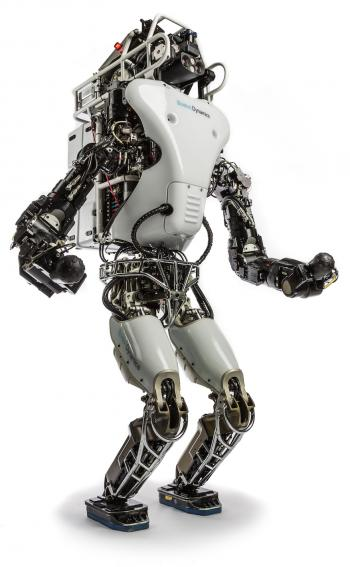
\includegraphics[width=4cm,height=6.5cm]{chapters/intro/images/atlas.jpg}}\quad
\end{subfigure}
\begin{subfigure}
[TORO]{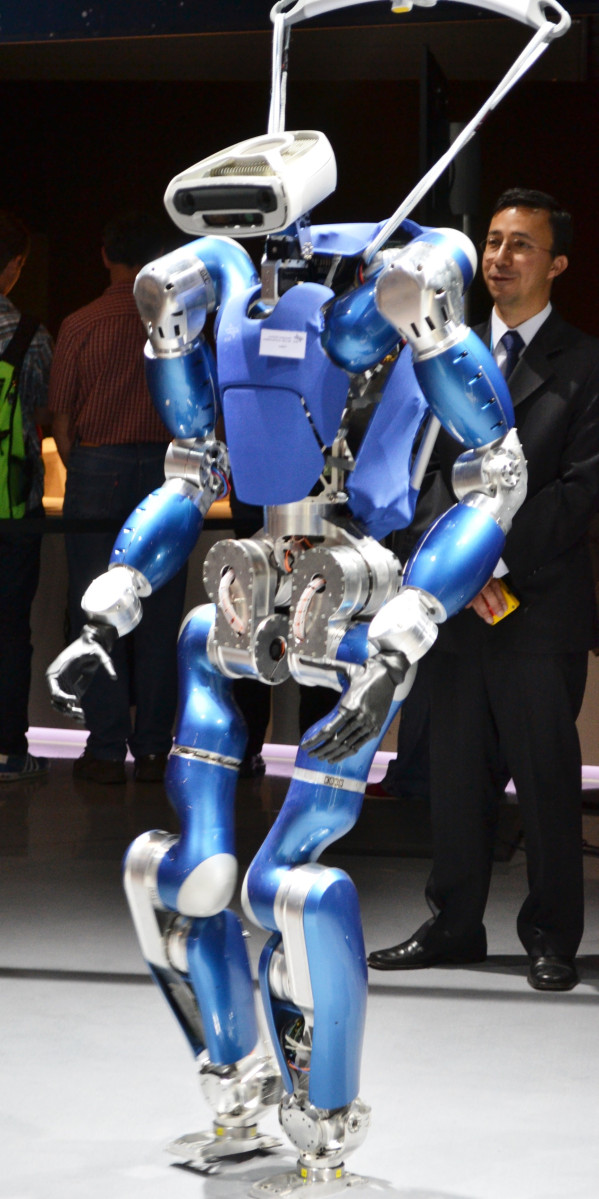
\includegraphics[width=4cm,height=6.5cm]{chapters/intro/images/toro.jpg}}\quad
\end{subfigure}
\begin{subfigure}
[TALOS]{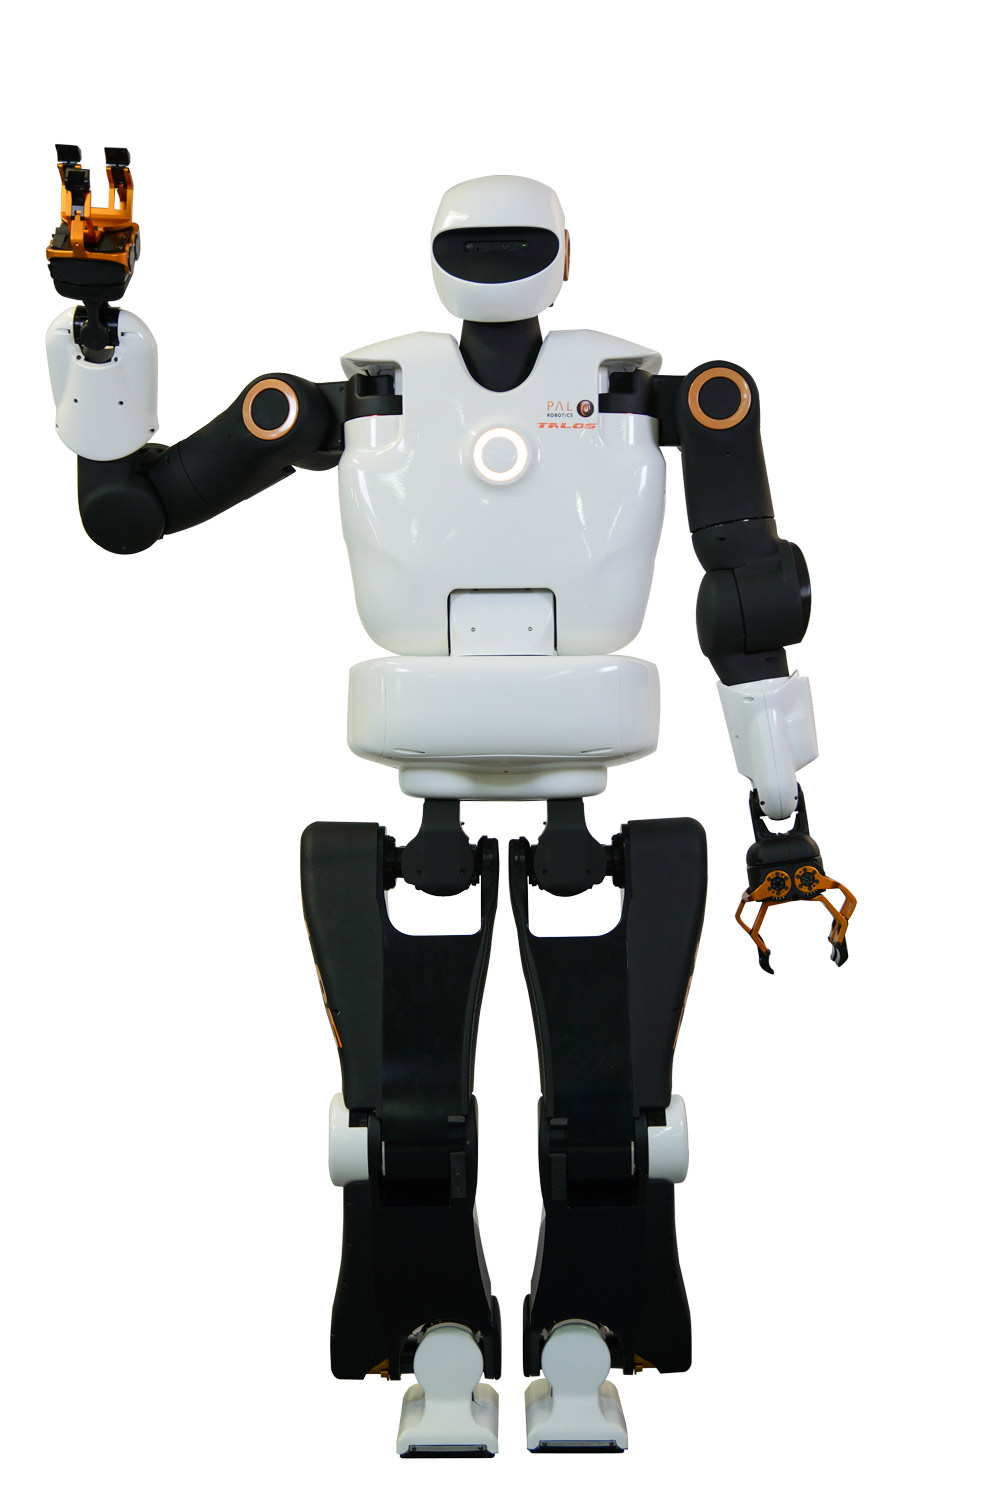
\includegraphics[width=4cm,height=6.5cm]{chapters/intro/images/talos.jpg}}\quad
\end{subfigure}
\caption{Latest Humanoid Robots}
\label{fig:hr_third}
\end{figure}

\subsection{Humanoids in Real Situations}
 Though there are a variety of humanoid robots with a lot of research going on, the applicability of those robots are quite limited. DRC competition challenged the limits of the humanoid robots by putting them in complex scenarios in dangerous environments. It is a great milestone in terms of the amount of attention the competition received and the participation of teams from different places in the world to solve problems in humanoid robotics. After filtering a lot of teams in the DRC simulation, 16 teams managed to contest in the trails. It involves a rich set of tasks that includes driving a utility vehicle, locomote across rubbles, remove debris, manipulate various tools such valves, fire hose and more. TEAM Kaist with their robot DRC-HUBO wont the contest. DRC has shown us how the robots perform in reality in spite of all the technologies working in controlled environment or in simulation. 


\begin{figure}[h]
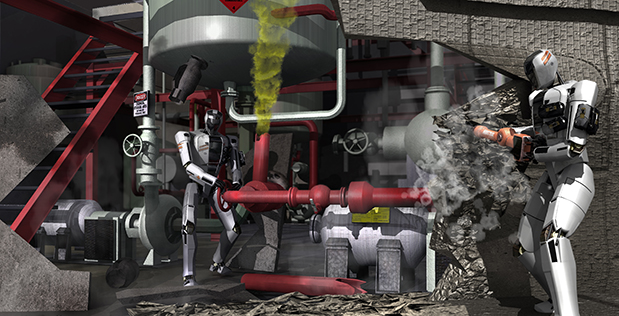
\includegraphics[scale=0.59,right]{chapters/intro/images/darpa.jpg}
\caption{DARPA Robotic Challenge}
\label{fig:darpa}
\end{figure}

The trails showed the lack of capabilities and functional robustness in task scenarios in spite of having tele-operators for guidance. The realization is that the technology is not matured enough and there are a plenty of problems to overcome. There are various aspects to these robot failures.
\begin{itemize}
    \item \textit{Robot Design}: The mechanical design of the robot has influence on the kind of failures it encounters with the environment. Walking on a flat surface is different from rough surfaces and an appropriate mechanical design is necessary to eliminate failures.

    \item \textit{Behavior Design}: The generated behaviors have to be robust to hardware failures. The kind of behaviors we choose have a big influence on the failures as well. This means robot should be able to handle variations in the task making the behavior robust. The whole body motion is also physically not depending on the external contacts. The robots usually have little or no ability to locomote using external contacts. For instance, it is very natural to hold the railings to climb up the stairs which reduces a significant amount of actuation in the joints.
    
    \item \textit{Human Robot Interaction}: When the human wants to control the robot in all the levels and switch between the modes easily, then it is not interaction anymore but intervention. Also trying to perform tasks as soon as possible puts the robot in a dynamic disadvantage.       
 
    \item \textit{Planning and Control}: Humanoid robots are redundant systems with more than 30 degrees of freedom which makes the whole body control complex. Also the pose of the robot can be only controlled indirectly by appropriate joint motions and its interaction with the environment making these robots under-actuated. 
    Constraint based inverse kinematics helps in handling control problems of humanoid robots but it is still challenging to eliminate undesired motions of the rest of the robot links while you execute the intended action in the task space. The physical interaction with the environment makes it more challenging to generate coordinated motions as it creates a variety of structural changes in the kinematics and dynamics of the robot changing the dimension of the problem. Switching control behaviors due to physical contact or joint limits or kinematic singularities challenges the limits of optimization solvers resulting in discontinuities in control. There is an ineffective use of foot torque/force sensors to close the control loop. All these problems make it easy for the robot to lose its balance.   
  
    \item \textit{Error Detection}: It is necessary to eliminate robot falls and they are mostly caused by errors generated by the system itself rather than perturbations from the environment. Detecting errors earlier can give a lot of time to take an appropriate control action to maintain balance. Though there are strategies available to handle external perturbations such as 'Push-Recovery' for example, robot generated errors are given less attention. Aborting the current behavior after detecting errors works but there is a necessity to handle them systematically. 

\end{itemize}

The above aspects shows the practical reality of the humanoid robots and the necessity of various components to function appropriately to be robust to failures. Balancing of legged robots is an essential safety constraint and the ability to handle failures is the motivation to focus on robust  balancing under inertial uncertainties of the robot model.  

\section{Control Methodologies in Humanoid Robotics}
\label{sec:control_methods}
Control methodologies in robotics generally define a control law that allows feasible motion generation with respect to both the robot and environmental constraints to achieve one or multiple desired tasks. There are a variety of methods to generate motion depending upon the robot, the environment and complexity of the task. The control of humanoid robots is quite specific and challenging because of the kinematic redundancy and the dynamic complexity of the system. They have a non-trivial kinematic tree structure with an essential need to stabilize the position of its center of mass(CoM) with respect to the feet at every moment while executing other tasks. In simple words, a humanoid robot cannot walk or run without knowing how to balance itself while in motion. 

Another challenging aspect to be considered here is that the dimension of task space does not equal the dimension of the actuators. Typical tasks consist in controlling the position and orientation of an end-effector (i.e. 6 dimensions), while a humanoid robot has more than 20 degrees of freedom. An inherent task-joint space mapping exists in the form of a trained nervous system in human beings but the robots need a very good dynamic model and appropriate cost functions to make deterministic interactions with the world. Humanoid robots are under-actuated systems which means their pose cannot be controlled directly but by a consequence of commanding appropriate trajectories in joint configuration space. In the following we discuss the state of the art 
approaches used in generating motions.

\subsection{Motion Planning}
Motion planning in robotics refers to the process of searching discrete and feasible motion sequences to achieve a desired task usually satisfying safety constraints and optimal criteria relevant to the task. A motion planning algorithm can be used to plan motion for a variety of tasks ranging from simple arm manipulation for 6 degree of freedom (DoF) robot arms \cite{donald1987search,lozano1987simple} to advanced walking pattern generation for legged robots \cite{kajita2003biped,huang2001planning,harada2006analytical}. The basic idea is to produce continuous motion sequences that connect a start and a goal configuration of the robot while avoiding collision with the obstacles and satisfying certain criteria specific to the task. 
\paragraph{Work Space}
The \textit{Work Space}(\WS) is the set of all robot positions that define the working volume of the robot end effector \cite{cao2011accurate}. This idea can be extended to mobile robot navigation or humanoid locomotion though the definition restricts to end effectors of robot manipulators. The robot and the obstacles are defined in the (\WS) but the motion is always computed or represented in the configuration space, which usually has higher dimension.  

\paragraph{Configuration Space}


The \textit{Configuration Space}(\CS{}) is the set of all configurations a robot can possibly attain. The \CS{} for a robot with \textit{n} degrees of freedom, is a manifold \M{} of \textit{n} dimensions with all robot configurations $q\in$\M{}. The important aspect is that the planning problem in a \WS{} of \sethree{} is transformed to a planning a point motion in its corresponding \CS{}. \CSobst{} represents the robot configurations that are self-colliding or in collision with the environment while \CSfree{} represents its complement. These subspaces allow the planning algorithm to search for a feasible path connecting the start and the end configuration avoiding collisions. 


\paragraph{Algorithms}Over the last 30 years, there has been a lot of research done in motion planning due to the variety of applications . A planning  algorithm is said to be complete if it can find a plan for all the instances of a problem when at least one exists, or report a failure if none exists. Computational complexity  is used to assess the performance of complete planning algorithms. Incomplete planners are not reliable though they are quite effective sometimes in practice. The algorithms can be categorized into \textit{deterministic} and \textit{sampling} based algorithms.
\begin{itemize}
\item \textit{Deterministic Algorithms}: These planning algorithms rely on a deterministic function to compute the path, always resulting in the same motion plan given the same planning request at any instant. Geometric approaches such as visibility graphs, cellular decomposition, Voronoi diagrams and Canny's algorithm compute the shape of \CSfree{} and its connectivity using graphs or road maps \cite{toth2004handbook,canny1988complexity} whereas Grid based approaches represents the configuration space in grids. They use search algorithms(such as $A^*$) to find a path based on the discrete number of actions within \CSfree{} region. These algorithms in general are computationally expensive for high dimensional configuration spaces. Potential field based methods \cite{barraquand1992numerical,koren1991potential} relies on artificially creaing an attractive potential field for the goal and a repulsive field to plan the instantaneous path. The approach is very efficient but it suffers from local minima. Reward based algorithms search for a path that maximizes the cumulative reward constrained by positive reward for reaching a goal and negative reward for collision with obstacles. Markov Decision Processes framework is used in most of the reward-based algorithms generating optimal path \cite{spaan2004point}. 
\item \textit{Sampling based Algorithms}: Sampling based algorithms approximate the connectivity of the feasible configurations in \CSfree{} by random sampling collision free configurations from \CS{} \cite{hudson1997v,gottschalk1996obbtree,hsu1997path}. \textit{Rapidly-exploring Random Trees}(RRT) is a quite popular algorithm which uses Voronoi bias to explore the free configuration space and grows a tree by sampling randomly at every iteration to connect the start and the goal point in \CSfree{}. In a slightly modified version referred to as \textit{Bi-directional RRT}, trees are grown from both the start and goal simultaneously to accelerate the process of the search \cite{kuffner2000rrt}. \textit{Probabilistic Roadmaps}(PRM) randomly sample from the \CS{} and connections are made with the neighbors generated by \textit{k} nearest neighbors or using a local planner \cite{karaman2011sampling}. A road map is developed by adding more configurations and connections until it is dense enough to be used for a planning problem. A path is searched or queried on the generated roadmap using Dijkstra's shortest path algorithm. There are a variety of PRM extensions to achieve better performance \cite{geraerts2004comparative}. Variations such as PRM* and RRT* for generic use cases preserve the asymptotic optimality of the tree \cite{karaman2011sampling}. Kinodynamic RRT* has been proposed for systems with controllable linear dynamics \cite{webb2013kinodynamic} and RRTs have been extended to LQR-Trees in state space \cite{tedrake2010lqr} and LQR-RRT* for linearized systems \cite{perez2012lqr}. Another extension \textit{Transition based RRT} uses stochastic optimization for computing potential states \cite{jaillet2008transition}. Sampling based algorithms deal with high dimensional configuration spaces and are probabilistically complete which means the probability that they fail to provide a solution approaches zero when more time is spent though there is no guarantee if a solution really exists or not.
\end{itemize}


Trajectory optimization is used to reduce the path length while preserving its validity. There are a variety of methods to optimize the trajectory such as greedy optimization \cite{thrun2002probabilistic}  which connects the start and the nearest node configuration that avoids obstacles in an iterative sequence until it reaches the goal configuration. 



\paragraph{Planning in Humanoid Robots}


As discussed before, Humanoid robots are under-actuated and balancing is essential to perform any other meaningful tasks. The motion planning algorithms described previously search for a collision free path considering only the geometry but do not really consider the effects of joint configurations on the whole robot itself. RRT algorithms are able to generate collision-free trajectories but do not optimize their smoothness or the associated control effort. There is a certain amount of control necessary to deterministically choose the right trajectories for tasks specific to a robot and the environment. So in humanoid robots or any polyarticulated system, inverse kinematic/dynamic or optimal control methodology can be used to generate trajectories under constraints. For instance, in humanoid robots it could be necessary to satisfy balance constraints under multiple contact while walking up the steps. In \cite{zhang2014motion}, predefined motion primitives guide the planner to generate natural trajectories.

With regard to Humanoid walking, deterministic planning approaches use a foot transition model with dynamic considerations and the trajectory smoothness during posture transitions \cite{chestnutt2005footstep,ayaz2007human} though there is no guarentee of completeness. Instead probobalistically complete methodologies like RRT can be used to search in discrete footsteps space \cite{perrin2012fast,xia2009random}. Goal-directed approaches such as in \cite{hornung2013search} ensures the path within bounded limits set by the optimal control solutions. Environment features such as contact points can also be used to guide planning \cite{bouyarmane2012dynamics,Escande2013}. There are also some approaches that decompose the problem from higher dimensions into smaller dimensions and are successively solved \cite{zhang2009motion,yoshida2008planning}. Planning is also done on constraint sub-manifolds within \CS{}. Approaches such as in \cite{bretl2006motion,hauser2010multi}, planning is done on union of sub-manifolds defined by balance constraints and leg positions for robots on uneven terrains. In \cite{berenson2011task}, they use jacobian based methods 
to add end effector pose constraints in a \textit{Constrained Bidirectional} RRT planner. In \cite{dalibard2013dynamic}, RRT is adapted within a random diffusion framework to generate statically stable trajectories. In recent times, path planning is combined with optimal contol to generate motion in cluttered environment \cite{el2013optimal}.

\subsection{Kinematic Control}
\paragraph{Basics of Robot Kinematics}
Kinematics is the study of movement of kinematic chains considering the geometry while ignoring the dynamic properties such as mass, inertia of the system and forces or torques to generate motion. The relationship between position, velocity and acceleration of the links of the system with respect to its kinematic connectivity and dimensionality is studied to control the movement of the system in joint space. The joint space of a robot with \textit{n} DoF is an \textit{n} dimensional manifold $\mathcal{Q}$ with all possible joint values. But in robotics, the pose of certain points are important for control in the task space. These point are generalized to \textit{Operational Points} \cite{Khatib1987}. The variation in an operational point x can be represented by a twist $\xi$ comprising linear and angular velocities \cite{featherstone2008rigid,Murray1994}. The kinematic control problem can be defined in four different ways:
\begin{itemize}
    \item \textit{Forward Kinematics}: Given a joint configuration $q \in \mathcal{Q}$, it involves finding the pose of an operational point $x \in SE(3)$ described by $x = f(q)$ such that $f:\mathcal{Q} \rightarrow SE(3)$. Denavit-Hartenberg(DH) parameters \cite{hartenberg1955kinematic} introduced in \cite{craig2005introduction} is quite a popular method used to represent the forward kinematics for serial manipulators though they are not suitable for closed kinematic chains and robot calibration \cite{khalil2004modeling,everett1987kinematic}. Other approaches include the \textit{Khalil-Kleinfinger} notations for closed loop robots \cite{khalil2004modeling}, \textit{Hayati-Roberts} coordinates for avoiding singularities \cite{hayati1985improving, roberts1988new}, screw theory modeling \cite{tsai1999robot}, product of exponentials(PoE) \cite{park1994computational} and methods 
    specific to humanoid robots as in \cite{kajita2005humanoid}.

    \item \textit{Forward differential kinematics}: Given a joint configuration variation $\dot{q} \in T_q(\mathcal{Q})$, it involves finding the twist of an operational point $\xi \in se(3)$ described by  $\xi = J_o(q)\dot{q}$ such that  $J_o:T_q(\mathcal{Q}) \rightarrow se(3)$ where $J_o$ is the tangent or geometric jacobian \cite{spong2006robot,Khatib1987} and $T_q(\mathcal{Q})$ is tangential to $\mathcal{Q}$ at $q$.
    \item \textit{Inverse Kinematics}: Given a pose $x \in SE(3)$ for an operational point, it involves finding the joint configuration
    $ q \in \mathcal{Q}$ described by $q = f^{-1}(x)$ such that $f^{-1}:SE(3) \rightarrow \mathcal{Q} $. The \textit{Inverse Kinematics} problem can be solved analytically for certain kinematic structures either using algebraic approaches as in \cite{paul1robot} \cite{RaghvanBoth1993inverse} or geometric approaches as in \cite{paden1985kinematics, peiper1968kinematics}.

    \item \textit{Inverse differential kinematics}: Given a twist $\xi \in se(3)$ for an operational point, it involves finding the 
    joint velocities $\dot{q} \in T_q(\mathcal{Q})$ described by $ \dot{q} = J_o(q)^{+}\xi$ where $J_o^{+}$ is a pseudo inverse such that $J_o^{+}:se(3) \rightarrow T_q (\mathcal{Q})$. It is solved analytically in \cite{Chiaverini1994,Chiaverini1997,siciliano1999tricept}  

\end{itemize}

\paragraph{Kinematic Redundancy}
The kinematic control involves reaching a reference point or tracking a trajectory in $SE(3)$ for one or more operational points by searching for the appropriate instantaneous joint configurations  $q(t)$. Such goals are called tasks. When the dimensions of the robot $n$ exceeds the task DoF $n_t$, the robot is said to be kinematically redundant with $n − n_t$ being the degree of redundancy with respect to task \cite{nakamura1990advanced}. Though it provides flexibility in the joint space to manage the constraints effectively, it is quite complex to handle the inverse kinematics in a multiple task scenario \cite{siciliano1991general}. Closed form solutions are not possible in redundant robots and choosing a solution that solves both the main and the complementary tasks as much as possible is essential. For instance, it is expected from a robotic arm to manipulate an object while avoiding collisions with the environmental obstacles reactively. Numerical approaches are used to solve these multi-task control problems on redundant robots.

Numerical methods formulate \textit{Inverse Kinematics} as a constrained optimization problem either globally or locally. Global methods search for an optimal path for the entire trajectory which is computational complex \cite{baillieul1990resolution}. Local methods solve them differentially computing locally optimal $dq$ for a small change $dx$ to generate the joint space trajectory $q(t)$. \textit{Resolved Motion Rate Control} in \cite{Whitney1969} finds the $\dot{q}$ by solving the system: $\dot{x} = J(q) \dot{q}$. Damped pseudo inverses \cite{nakamura1986inverse} are used to avoid singularities and inversion issues in redundant robots when the Jacobian is not a full row or column rank matrix. 

 A more generic solution solves each task by projecting onto the nullspace of the Jacobian $J$ supplying certain degrees of freedom to the specific task \cite{Liegeois1977}. There are two ways to carry out the projection systematically.

 \begin{itemize}
     \item \textit{Task Space Augmentation} uses weighting to modulate the task space by constraining the joint space\cite{sciavicco1987solving}. Task conflicts are managed by assigning weights to each task making a compromise between the goals of the tasks.  Proper tuning specific to the scenario is essential for this methodology. \textit{Extended Jacobian Matrix} helps in handling the conflict between tasks by zeroing down the projection of the cost function gradient on the null space of the Jacobian \cite{baillieul1985kinematic}.

     \item \textit{Task Prioritization} strictly prioritizes the projection hierarchically by ensuring that the lower priority task do not affect the tracking error of the higher priority task \cite{nakamura1987task}. A systematic framework for a multi-task scenarios is proposed in \cite{siciliano1991general} which algorithmically generates $\dot{q}$ to minimize the task error in a prioritized way. A solution in \cite{Baerlocher1998} is used to speed up the computation of null space projector. 
     
 \end{itemize}

\paragraph{Redundancy Resolution in Humanoid Robots}
Since humanoids and redundant robots have a tree like structure, closed form solutions are generated by treating the complete robot as a set of many kinematic chains as in \cite{ali2010closed,nunez2012explicit}. These approaches are quite complex and instantaneous inverse kinematic solvers are usually preferred. Linearizing the problem on humanoid robot, produces infinite solutions providing the possibility to perform multiple tasks. \textit{Task Space Augmentation} methods as in \cite{tevatia2000inverse} and \cite{salini2009lqp} suffer from task conflicts resulting in unsuccessful task execution whereas \textit{Task Space Prioritization} has a strict priority on resolving multiple tasks leading to locally optimal results.
 The method is also computationally less expensive and are used in common. Several approaches have been developed for multiple equality constraints at the kinematic level \cite{yoshida2006task,mansard2007task,gienger2005task}. For inequality tasks, sequential quadratic programming is used to solve a cascade of tasks \cite{kanoun2009prioritizing}. A much more efficient implementation using complete orthogonal decomposition
is proposed by \cite{Escande2014} which the state of the art solver Stack of Tasks used to solve a hierarchical quadratic program. \cite{jarquin2013real} also proposes a solution for a smooth transition in control when the priorities are interchanged.  


\subsection{Dynamic Control}

\paragraph{Basics of Robotic Dynamics}
Dynamics is the study of the dynamic relationship between the motion of the kinematic chain and the generalized forces acting on the system to make movement. The generalized forces are the external forces applied to the system which include the joint torques for rotational joints, joint forces for prismatic joints, and also the force due to external contacts. This relationship allows to control the robot in a dynamic level enabling a better interaction with the environment. Dynamic parameters such as length, mass, inertia of the links and the forces or torques acting on the mechanical system are considered. In a robot dynamic model, the motion is defined by joint  acceleration $\ddot{q}$ and operational point acceleration $\ddot{x}$ in the task space. 

\begin{itemize}
    \item \textit{Forward Dynamics} determines the acceleration of the robot in the joint space when generalized forces are applied in the joint space
    \item \textit{Inverse Dynamics} determines the generalized forces necessary in joint space to achieve a required acceleration in the joint space.
\end{itemize}

The two main approaches to model the robot dynamics are:

\begin{itemize}
    \item \textit{Lagrange Method} is energy based with dynamic equations in closed form. \cite{uicker1969dynamic,kahn1969near,bejczy1974robot} are such approaches in the robotics domain. It has a clear separation of each component but it is very expensive  for implementing control schemes. \cite{hollerbach1980recursive} presents an efficient formulation but still \textit{Newton-Euler Method} are preferred for faster computation.
    \item \textit{Newton-Euler Method} is a generalized force based and recursive in nature. The first of its kind is presented in \cite{orin1979kinematic}. It does not clearly separate components but it is computationally cheaper. \cite{Featherstone2009} explains the most common algorithms such as the composite-rigid-body algorithm (CRBA), the articulated-body algorithm (ABA), the recursive Newton-Euler Algorithm (RNEA). 
\end{itemize}
\cite{spong1992remarks} uses an hamiltonian approach for the analysis of the robot dynamics and there exist certain numerical methods to integrate hamiltonian equations efficiently. Alternatively, \textit{Centroidal dynamics} \cite{orin2013centroidal,orin2008centroidal} models the dynamics of the CoM of the robot capturing the constraints imposed by contact forces on the CoM making the dynamic model very simple. But it does not include joint position and torque limits which makes the model approximate failing to describe the angular momentum of the robot. Humanoids walk with very little angular momentum and is set to zero applying when \textit{Centroidal dynamics} .
In contrast to the classic joint space formulation, the operational space formulation \cite{Khatib1987} defines the motion using the task space acceleration, which requires the forces to be formulated as generalized forces in the task space.

\paragraph{Dynamic Control in Humanoid Robotics}
As discussed already, classical techniques are not appropriate for humanoid robots as the control scheme has to execute coordinated motion keeping into account the interaction forces exchanged with the environment along with balance all the time. Stability criteria that constrain the CoM or the zero moment point (ZMP) within the support polygon are often enforced in the controller \cite{wieber2002stability}. A constraint on the ZMP is equivalent to a constraint on the tangential moment at the contact surfaces. The interaction of legs on the ground along with other contacts of the robot body with the environment is also necessary. The contact forces are transformed to generalized forces on the joints which can be controlled only using joint torque control. Dynamic control is quite essential in ensuring motion feasibility, agility and balance in 
humanoid robots.

The operational-space inverse-dynamics (OSID), a generic framework  establishes the whole-body control considering balance, contacts and other constraints. \cite{Khatib2004} proposes a multi-task formulation with sequential projection on  the nullspaces of the tasks at each level. Strict hierarchy allows lower priority tasks not to affect the higher priority tasks. An equivalent approach \cite{mistry2010inverse} uses orthogonal decomposition and kinematic projections to simply control when switching contact constraints and avoids the inversion of mass matrix. \cite{Righetti2011a,Righetti2011} proposes an improved version constraining the ground reaction forces with the friction boundaries. Inequality constraints can not be added in this framework which is quite necessary to implement collision avoidance, joint limits and visual servoing task. OSID's are used within optimization based methodologies to find optimal solutions. Quadratic Programming (QP) based approaches are more popular for redundant systems which allows both equality and inequality tasks. Weighting schemes are used in a QP based approach which provides robust balance \cite{collette2008robust}. \cite{Salini2011} implements a weighting focused on the task prioritization. Decoupling of the dynamics in holonomic and non-holonomic part is used in a QP to generate feasible whole body trajectories \cite{bouyarmane2012dynamics,wieber2006holonomy}. \cite{herzog2013experiments} uses active set method to implement a torque control of the lower part of the robot. OSID in a strictly prioritized QP framework is implemented in \cite{Saab2013}. 


The previous approaches focused on the robot dynamics but the angular momentum was not controlled specifically which is an important part of motion in human beings doing agile and complex motion \cite{popovic2004angular}. \cite{kajita2003resolved} proposed to control the angular momentum of the robot using the inverse of the inertia matrix. \textit{Centroidal dynamics} controls the angular momentum as in \cite{hofmann2009exploiting} focusing on gait movements and \cite{moro2013attractor} where an attractor is used to control. Also \cite{wensing2013generation} uses conic optimization techniques to control the angular momentum generating complex motions.

\subsection{Optimal Control}
Optimal Control involves finding control laws for a given system such that certain optimality criteria are minimized. It is a problem of searching trajectories that satisfy the system dynamics and minimizing a cost function. In Robotics, it is also called as \textit{Trajectory Optimization} or \textit{Trajectory Filtering}.

\paragraph{Background}
Optimal Control is actually an extension of a theory of \textit{Calculus of Variations} that uses optimization methodologies to find control policies. The first ever optimal control solution was proposed for the brachystochrone problem in Bernouli's work. Though there were early contributions to the theory of optimal control by Newton, Euler, Leibniz, Jacobi, Hamilton, Bolza and many others, the formalization began to take shape with the introduction of Linear Quadratic Control(LQC) problem minimizing a squared error of an expected value of a random variable x \cite{wiener1949extrapolation}. The next milestone was the birth of Dynamic Programming (DP) to solve discrete time optimal control problems which reduces the search to Hamilti-Jacobian equation. The formulation of the Pontryagin maximum principle \cite{pontryagin1987mathematical} completely formalize the problem based on the calculus of variations considering  pathwise constraints on control values of the functions. \textit{Linear Quadratic Regulator (LQR)} and the \textit{Linear Quadratic Gaussian (LQG)} are formulated to design optimal control policies in \cite{Kalman1960} which marks another important formulation in optimal control.

\textit{Model Predictive Control (MPC)} also called as Receding Horizon Control is a popular automatic control methodlogy in industries which uses the optimal control solution at each instant over a time horizon called the prediction horizon \cite{richalet1978model}. Task specific goals are specified by simple penalty functions in the optimal control which synthesizes the motion behaviour and control laws. The controller predicts the futures states under certain criteria which lets them find the control values to achieve the appropriate current state avoiding extensive exporation. \textit{Differential Dynamic Programming(DDP)} is a numerical scheme quite efficient for direct implicit optimal control generating local trajectories \cite{jacobson1968new}. A hybrid method uses constant local controllers \cite{atkeson1994using} which is improvized in \cite{atkeson2003nonparametric} using second order local models to make linear controllers.


\paragraph{Optimal Control in Humanoid Robotics}
For humanoid robot walking, the \textit{Operational Space Inverse Dynamics} or \textit{Inverse Kinematics} cannot really handle the accelerations of the CoM properly thus generating very conservative or over restricted motion. Optimal control can find 
trajectories from initial to final posture specified as one complete objective or many objectives with certain constraints. Optimal control can generate proper and powerful trajectories for CoM unlike IK or OSID. It is quite equivalent to a classical walking pattern generator in addition to the ability to incorporate whole body motion. MPC's are a quite relevant control scheme in humanoid robotics and control solutions as in \cite{kajita2003biped,herdt2010online} uses a dedicated Linearize Inverted Pendulum model to predict the future state of the system for controlling dynamic stability. Though it is quite complex and the models have to be created for every new case, optimal control is very appropriate and takes care of all the constraints at the same horizon. One problem with using optimal control in humanoid robotics is the computational time because of more DoFs and it requires a faster response when controlled in dynamic level.

In multiple task scenarios, weighted average of tasks can be used to influence the priority by choosing right weights for each task in the set \cite{dimitrov2011sparse}. It obviously introduces task conflicts if the relative difference of the weights are not significantly high. Large weights can also produce numerical errors resulting in pracitcal complexity to implement such control schemes. In \cite{del2014prioritized}, the optimal control is strictly prioritized avoding such issues. MuJoCo is a state of the art simulator that uses MPC to generate humanoid trajectories with high computational speed with respect to dynamic derivatives\cite{todorov2012mujoco}. Behaviours like getting up from the ground and avoiding disturbances were generated in this simulator \cite{tassa2012synthesis}.  The use of environment increases the controllable space to successively acheive the goals as in \cite{lengagne2013generation} generating non-coplanar contact motions. Parkour motion\cite{dellin2012framework}, kicking a ball \cite{miossec2006development} and  lifting weights \cite{arisumi2008dynamic} shows some application of optimal control in generating complex behaviours.

Variants of DDP exist with respect to optimal control in humanoid robots. Control-limited DDP allows adding inequality constraints as proposed in \cite{tassa2014control}  has been applied on a humanoid robot in simulation. Square-root DDP proposed in \cite{geoffroy2014inverse} shows that IK and OSID are special cases of optimal control without preview horizon. DDP is also used in generating sample trajectories to learn a neural network based guided policy to avoid local minima in \cite{Levine2012}. Behaviors such as walking, running, hopping and swimming are generated using this approach. Robust walking behaviours were generated using DP in \cite{whitman2013coordination} relying on multi model and learning based DP variants. Steep climbing motion is generated in \cite{Noda2014}
which uses Body Retention Load Vector to model the physical constraints. Optimal control has also been treated as an offline control problem in \cite{schultz2010modeling} optimizing energy based criteria using multiple shooting approach to generate running behaviors. Walking motions are generated without using a pattern generator but just by optimizing joint velocities, torques or ZMP constraints \cite{el2013optimal,koch2012studying}. Inverse optimal control involves learning the criteria to generate observed motions in a dynamic system. Human locomotion is studied using inverse optimal control in one such work \cite{mombaur2010human}. Also human running is studied in different terrains and distirubances in \cite{park2013inverse}


Motion planning is also combined with optimization for collision free navigation in a cluttered environment. Motion planners for high DoF systems generate trajectory in two stages: planning and optimization. There are three well known and similar techniques in this domain. CHOMP (Covariant Hamiltonian Optimization for Motion Planning) uses covariant gradient descent technique in the solver resulting in a planning algorithm completely relying on trajectory optimization \cite{zucker2013chomp}. Starting with a naive trajectory, CHOMP optimizes the dynamics of the trajectory while reacting to the obstacles in the environment. STOMP (Stochastic Trajectory Optimization for Motion Planning) is very similar except for the use of trajectory stochastic perturbations to generate trajectories without computing the jacobian \cite{kalakrishnan2011stomp}. ITOMP (Incremental Trajectory Optimization for Real-Time Replanning in Dynamic Environments) can produce suboptimal solutions because of the time constraints on the solver and the trajectory is incrementally updated online \cite{park2014high}.

High dimensionality is challenging in humanoid robotics to get optimal control working in real time. The state space gets large due to high number of DoFs and it is not easy to explore all of it apriori and generate appropriate trajectories for every cases. Current optimal control solutions are time consuming and encounters numerical problems which is sill an open issue in robotics.

\section{Chapter Organization}
The thesis has two main chapters \ref{chapter:framework} and \ref{chapter:rc} describing the two main contributions of this thesis respectively. Chapter \ref{chapter:framework} presents the dynamic obstacle framework developed on industrial robots for collision avoidance using proximity information from skin sensors and point cloud information from 3d cameras. The Chapter \ref{chapter:rc} presents the strategy used to model inertial uncertainties to perform robust balancing. Chapter 5 concludes the thesis with important comments on the contributions and the possible future work connected to it.
\section{Publications}
\begin{itemize}
\item Giftsun, N., Prete, A. Del, \& Lamiraux, F. (2017). \textit{Robustness to Inertial Parameter Errors for Legged Robots Balancing on Level Ground.} International Conference on Informatics in Control, Automation and Robotics (ICINCO) \textbf{[CONFERENCE]}.
\item Bharatheesha, M., Giftsun, N., Hernandez, C., Bergner, F., Dean-leon, E., \& Cheng, G. (2017). \textit{Dynamic Obstacle Avoidance for Collaborative Robot Applications.} IEEE International Conference on Robotics and Automation (ICRA)\textbf{[WORKSHOP]}.
\end{itemize}
\ifdefined\included
\else
\bibliographystyle{acm}
\bibliography{These}
\end{document}
\fi


\ifdefined\included
\else
\documentclass[a4paper,11pt,twoside]{StyleThese}
\usepackage{amsmath,amssymb}             % AMS Math
\usepackage[T1]{fontenc}
\usepackage[utf8x]{inputenc}
\usepackage{babel}
\usepackage{datetime}

\usepackage{lmodern}
\usepackage{tabularx}
%\usepackage{tabular}
\usepackage{multirow}

\usepackage{hhline}
\usepackage[left=1.5in,right=1.3in,top=1.1in,bottom=1.1in,includefoot,includehead,headheight=13.6pt]{geometry}
\renewcommand{\baselinestretch}{1.05}

% Table of contents for each chapter

\usepackage[nottoc, notlof, notlot]{tocbibind}
\usepackage{minitoc}
\setcounter{minitocdepth}{2}
\mtcindent=15pt
% Use \minitoc where to put a table of contents

\usepackage{aecompl}

% Glossary / list of abbreviations

\usepackage[intoc]{nomencl}
\iftoggle{ThesisInEnglish}{%
\renewcommand{\nomname}{Glossary}
}{ %
\renewcommand{\nomname}{Liste des Abréviations}
}

\makenomenclature

% My pdf code

\usepackage{ifpdf}

\ifpdf
  \usepackage[pdftex]{graphicx}
  \DeclareGraphicsExtensions{.jpg}
  \usepackage[a4paper,pagebackref,hyperindex=true]{hyperref}
  \usepackage{tikz}
  \usetikzlibrary{arrows,shapes,calc}
\else
  \usepackage{graphicx}
  \DeclareGraphicsExtensions{.ps,.eps}
  \usepackage[a4paper,dvipdfm,pagebackref,hyperindex=true]{hyperref}
\fi

\graphicspath{{.}{images/}}

%% nicer backref links. NOTE: The flag ThesisInEnglish is used to define the
% language in the back references. Read more about it in These.tex

\iftoggle{ThesisInEnglish}{%
\renewcommand*{\backref}[1]{}
\renewcommand*{\backrefalt}[4]{%
\ifcase #1 %
(Not cited.)%
\or
(Cited in page~#2.)%
\else
(Cited in pages~#2.)%
\fi}
\renewcommand*{\backrefsep}{, }
\renewcommand*{\backreftwosep}{ and~}
\renewcommand*{\backreflastsep}{ and~}
}{%
\renewcommand*{\backref}[1]{}
\renewcommand*{\backrefalt}[4]{%
\ifcase #1 %
(Non cité.)%
\or
(Cité en page~#2.)%
\else
(Cité en pages~#2.)%
\fi}
\renewcommand*{\backrefsep}{, }
\renewcommand*{\backreftwosep}{ et~}
\renewcommand*{\backreflastsep}{ et~}
}

% Links in pdf
\usepackage{color}
\definecolor{linkcol}{rgb}{0,0,0.4} 
\definecolor{citecol}{rgb}{0.5,0,0} 
\definecolor{linkcol}{rgb}{0,0,0} 
\definecolor{citecol}{rgb}{0,0,0}
% Change this to change the informations included in the pdf file

\hypersetup
{
bookmarksopen=true,
pdftitle="Évaluation de la sécurité des équipements grand public connectés à Internet",
pdfauthor="Yann BACHY", %auteur du document
pdfsubject="Thèse", %sujet du document
%pdftoolbar=false, %barre d'outils non visible
pdfmenubar=true, %barre de menu visible
pdfhighlight=/O, %effet d'un clic sur un lien hypertexte
colorlinks=true, %couleurs sur les liens hypertextes
pdfpagemode=None, %aucun mode de page
pdfpagelayout=SinglePage, %ouverture en simple page
pdffitwindow=true, %pages ouvertes entierement dans toute la fenetre
linkcolor=linkcol, %couleur des liens hypertextes internes
citecolor=citecol, %couleur des liens pour les citations
urlcolor=linkcol %couleur des liens pour les url
}

% definitions.
% -------------------

\setcounter{secnumdepth}{3}
\setcounter{tocdepth}{2}

% Some useful commands and shortcut for maths:  partial derivative and stuff

\newcommand{\pd}[2]{\frac{\partial #1}{\partial #2}}
\def\abs{\operatorname{abs}}
\def\argmax{\operatornamewithlimits{arg\,max}}
\def\argmin{\operatornamewithlimits{arg\,min}}
\def\diag{\operatorname{Diag}}
\newcommand{\eqRef}[1]{(\ref{#1})}

\usepackage{rotating}                    % Sideways of figures & tables
%\usepackage{bibunits}
%\usepackage[sectionbib]{chapterbib}          % Cross-reference package (Natural BiB)
%\usepackage{natbib}                  % Put References at the end of each chapter
                                         % Do not put 'sectionbib' option here.
                                         % Sectionbib option in 'natbib' will do.
\usepackage{fancyhdr}                    % Fancy Header and Footer

% \usepackage{txfonts}                     % Public Times New Roman text & math font
  
%%% Fancy Header %%%%%%%%%%%%%%%%%%%%%%%%%%%%%%%%%%%%%%%%%%%%%%%%%%%%%%%%%%%%%%%%%%
% Fancy Header Style Options

\pagestyle{fancy}                       % Sets fancy header and footer
\fancyfoot{}                            % Delete current footer settings

%\renewcommand{\chaptermark}[1]{         % Lower Case Chapter marker style
%  \markboth{\chaptername\ \thechapter.\ #1}}{}} %

%\renewcommand{\sectionmark}[1]{         % Lower case Section marker style
%  \markright{\thesection.\ #1}}         %

\fancyhead[LE,RO]{\bfseries\thepage}    % Page number (boldface) in left on even
% pages and right on odd pages
\fancyhead[RE]{\bfseries\nouppercase{\leftmark}}      % Chapter in the right on even pages
\fancyhead[LO]{\bfseries\nouppercase{\rightmark}}     % Section in the left on odd pages

\let\headruleORIG\headrule
\renewcommand{\headrule}{\color{black} \headruleORIG}
\renewcommand{\headrulewidth}{1.0pt}
\usepackage{colortbl}
\arrayrulecolor{black}

\fancypagestyle{plain}{
  \fancyhead{}
  \fancyfoot{}
  \renewcommand{\headrulewidth}{0pt}
}

%\usepackage{MyAlgorithm}
%\usepackage[noend]{MyAlgorithmic}
\usepackage[ED=MITT - STICRT, Ets=INSA]{tlsflyleaf}
%%% Clear Header %%%%%%%%%%%%%%%%%%%%%%%%%%%%%%%%%%%%%%%%%%%%%%%%%%%%%%%%%%%%%%%%%%
% Clear Header Style on the Last Empty Odd pages
\makeatletter

\def\cleardoublepage{\clearpage\if@twoside \ifodd\c@page\else%
  \hbox{}%
  \thispagestyle{empty}%              % Empty header styles
  \newpage%
  \if@twocolumn\hbox{}\newpage\fi\fi\fi}

\makeatother
 
%%%%%%%%%%%%%%%%%%%%%%%%%%%%%%%%%%%%%%%%%%%%%%%%%%%%%%%%%%%%%%%%%%%%%%%%%%%%%%% 
% Prints your review date and 'Draft Version' (From Josullvn, CS, CMU)
\newcommand{\reviewtimetoday}[2]{\special{!userdict begin
    /bop-hook{gsave 20 710 translate 45 rotate 0.8 setgray
      /Times-Roman findfont 12 scalefont setfont 0 0   moveto (#1) show
      0 -12 moveto (#2) show grestore}def end}}
% You can turn on or off this option.
% \reviewtimetoday{\today}{Draft Version}
%%%%%%%%%%%%%%%%%%%%%%%%%%%%%%%%%%%%%%%%%%%%%%%%%%%%%%%%%%%%%%%%%%%%%%%%%%%%%%% 

\newenvironment{maxime}[1]
{
\vspace*{0cm}
\hfill
\begin{minipage}{0.5\textwidth}%
%\rule[0.5ex]{\textwidth}{0.1mm}\\%
\hrulefill $\:$ {\bf #1}\\
%\vspace*{-0.25cm}
\it 
}%
{%

\hrulefill
\vspace*{0.5cm}%
\end{minipage}
}

\let\minitocORIG\minitoc
\renewcommand{\minitoc}{\minitocORIG \vspace{1.5em}}

\usepackage{multirow}
%\usepackage{slashbox}

\newenvironment{bulletList}%
{ \begin{list}%
	{$\bullet$}%
	{\setlength{\labelwidth}{25pt}%
	 \setlength{\leftmargin}{30pt}%
	 \setlength{\itemsep}{\parsep}}}%
{ \end{list} }

\newtheorem{definition}{Définition}
\renewcommand{\epsilon}{\varepsilon}

% centered page environment

\newenvironment{vcenterpage}
{\newpage\vspace*{\fill}\thispagestyle{empty}\renewcommand{\headrulewidth}{0pt}}
{\vspace*{\fill}}

\usepackage{tablefootnote}

\usepackage{hyperref}
\hypersetup{
     colorlinks   = true,
     citecolor    = violet
}
\usepackage{graphicx} % for pdf, bitmapped graphics files
\usepackage{amsmath} % assumes amsmath package installed
\usepackage{amssymb}  % assumes amsmath package installed
\usepackage{bm} % for using bold lowercase greek letters
\usepackage{array}
\usepackage{colortbl}	% to color table background
%\usepackage[table]{xcolor}
\usepackage{subfigure}  
\usepackage{tikz}
\newcommand{\tikzcircle}[2][red,fill=red]{\tikz[baseline=-0.5ex]\draw[#1,radius=#2] (0,0) circle ;}%
\definecolor{turquoise}{rgb}{0.28 1 0.92}
\newcommand{\fratop}[2]{\genfrac{}{}{0pt}{}{#1}{#2}}
\newcommand{\mx}[1]{\mathbf{\bm{#1}}} 				% Matrix symbol
\newcommand{\vc}[1]{\mathbf{\bm{#1}}} 					% Vector symbol
\newcommand{\degree}{\ensuremath{^\circ}}				% define the degree symbol
\newcommand{\pder}[2]{\frac{\partial#1}{\partial#2}}		% partial derivative
\newcommand{\ppder}[2]{\frac{\partial^2 #1}{\partial#2^2}}		% second partial derivative
\newcommand{\refframe}[1]{\mbox{\textless#1\textgreater}}	% to denote a reference frame
%\DeclareMathOperator*{\lexmin}{\text{lex}\!\min}			% lexmin
\DeclareMathOperator*{\minimize}{minimize}				% minimize
\DeclareMathOperator*{\maximize}{maximize}				% maximize
%\DeclareMathOperator*{\argmin}{\arg\!\min}				% argmin
%\DeclareMathOperator*{\argmax}{\arg\!\max}				% argmax
\DeclareMathOperator*{\st}{subject\,to}					% subject to
\DeclareMathOperator*{\dif}{\mathrm{d}}					% d
\DeclareMathOperator*{\half}{\frac{1}{2}}					% one half
\newcommand{\mat}[1]{\ensuremath{\begin{bmatrix}#1\end{bmatrix}}}	% matrix
\newcommand{\rank}[1]{\text{rank}(#1)}							% rank
%\newcommand{\diag}[1]{\text{diag}(#1)}							% diag
\newcommand{\x}{\ensuremath{\times}}
\newcommand{\spac}{\ensuremath{\quad}}						% alias for space in math environment
\newcommand{\dt}[0]{\ensuremath{\Delta t}}					% dt
\newcommand{\dx}[0]{\ensuremath{\delta x}}					% dx
\newcommand{\du}[0]{\ensuremath{\delta u}}					% du
\newcommand{\dhu}[0]{\ensuremath{\delta \hat{u}}}					% \hat{du}
\newcommand{\dbu}[0]{\ensuremath{\delta \bar{u}}}					% \bar{du}
\newcommand{\dtu}[0]{\ensuremath{\delta \tilde{u}}}					% \tilde{du}
\newcommand{\dhx}[0]{\ensuremath{\delta \hat{x}}}					% \hat{dx}
\newcommand{\DX}[0]{\ensuremath{\Delta X}}						% DX
\newcommand{\DU}[0]{\ensuremath{\Delta U}}						% DU
\newcommand{\Ts}[0]{\ensuremath{\top}}							% transpose symbol
\newcommand{\pinv}[0]{\ensuremath{\dagger}}					% pseudoinverse symbol
\newcommand{\Rv}[1]{\ensuremath{\mathbb{R}^{#1}}}				% set of real-valued vectors
\newcommand{\Rm}[2]{\ensuremath{\mathbb{R}^{#1\times #2}}}		% set of real-valued matrices
\newcommand{\Spd}[1]{\ensuremath{\mathbb{S}_+^{#1}}}			% set of symmetric positive-definite matrices
\newcommand{\card}[1]{\ensuremath{\left\vert{#1}\right\vert}}			% cardinality of a set
\DeclareMathOperator{\Tr}{Tr}							% trace
\newcommand{\Expect}{{\rm I\kern-.3em E}}				% expectation
\newcommand{\Normal}{\mathcal{N}}					% normal distribution
\newcommand{\Prob}[1]{\text{P}(#1)}						% probability
\newcommand{\vech}[1]{\text{vech}(#1)}						% vech

\newcommand{\sethree}{\ensuremath{SE(3)}}
\newcommand{\CS}{$\mathcal{CS}$}
\newcommand{\WS}{$\mathcal{WS}$}
\newcommand{\CSfree}{$\mathcal{CS}_{free}$}
\newcommand{\CSobst}{$\mathcal{CS}_{obst}$}
\newcommand{\M}[0]{$\mathcal{M}$}

%\algnewcommand{\algorithmicgoto}{\textbf{go to}}%
%%\algnewcommand{\Goto}[1]{\algorithmicgoto~\ref{#1}}%
%\algnewcommand{\Goto}{\algorithmicgoto\xspace}%
%\algnewcommand{\Label}{\State\unskip}

\newenvironment{definition}[1][Definition]{\begin{trivlist}
\item[\hskip \labelsep {\bfseries #1}]}{\end{trivlist}}

\usepackage{epstopdf}
\usepackage[colorinlistoftodos,prependcaption,textsize=tiny]{todonotes}
\newcommand\explainmore[1]{\textcolor{red}{#1}}
\newcommand\refrephrase[1]{\textcolor{yellow}{#1}}
\newcommand\donerephrasing[1]{\textcolor{green}{#1}}

%DIF PREAMBLE EXTENSION ADDED BY LATEXDIFF
%DIF UNDERLINE PREAMBLE %DIF PREAMBLE
\RequirePackage[normalem]{ulem} %DIF PREAMBLE
\RequirePackage{color}\definecolor{RED}{rgb}{1,0,0}\definecolor{BLUE}{rgb}{0,0,1} %DIF PREAMBLE
\providecommand{\DIFadd}[1]{{\protect\color{blue}\uwave{#1}}} %DIF PREAMBLE
\providecommand{\DIFdel}[1]{{\protect\color{red}\sout{#1}}}                      %DIF PREAMBLE
%DIF SAFE PREAMBLE %DIF PREAMBLE
\providecommand{\DIFaddbegin}{} %DIF PREAMBLE
\providecommand{\DIFaddend}{} %DIF PREAMBLE
\providecommand{\DIFdelbegin}{} %DIF PREAMBLE
\providecommand{\DIFdelend}{} %DIF PREAMBLE
%DIF FLOATSAFE PREAMBLE %DIF PREAMBLE
\providecommand{\DIFaddFL}[1]{\DIFadd{#1}} %DIF PREAMBLE
\providecommand{\DIFdelFL}[1]{\DIFdel{#1}} %DIF PREAMBLE
\providecommand{\DIFaddbeginFL}{} %DIF PREAMBLE
\providecommand{\DIFaddendFL}{} %DIF PREAMBLE
\providecommand{\DIFdelbeginFL}{} %DIF PREAMBLE
\providecommand{\DIFdelendFL}{} %DIF PREAMBLE
%DIF END PREAMBLE EXTENSION ADDED BY LATEXDIFF


\begin{document}


\sloppy
\begin{document}
\setcounter{chapter}{0} %% Numéro du chapitre précédent ;)
\fi

\chapter{Collision Avoidance Framework}
\label{chapter:framework}
Current collaborative robot arms allow more flexible work cells, where they safely collaborate with human operators augmenting productivity in tasks difficult for traditional automation. However, current robotic solutions for safe interaction simply stops the robot motion when a collision is detected. This reduces the productivity in an operational setup in which unintended, safe collisions can happen often. Active contact evasion by the robot arm is desired so that the production process continues despite regular interferences and path obstructions without compromising on the human safety. In Factory-in-a-day project, technologies to avoid collisions dynamically in a manipulation setup have been developed which includes proximity-measuring robot skin, reactive path-planning \& motion control components to generate collision free motions in a real time industrial setup. These technologies have been integrated into a unifying framework for dynamic collision avoidance which is successfully tested both in simulation and laboratory set-ups. The primary contribution of this thesis is a robust reactive control mechanism using the state of the art kinematic Hierarchical Quadratic Programming(HQP) solver to handle safety constraints determined by proximity skin information. This chapter makes an attempt to summarize the various developments relevant to collision avoidance, presents the proposed framework developed in the Factory-in-a-day project with a special focus on the reactive control components.
\section{Introduction}
A desire for robotic solutions, particularly in the small and medium scale enterprises (SMEs) is becoming increasingly prominent. Automation and robotics promise to deliver reduction on production costs and increase in productivity. However, traditional automation implies an investment prohibitive for SMEs, whose activities mainly involve small batches of production and high variety of products, for example, due to a seasonal nature of their operations. Concretely, tasks such as assembly, machine filling or packaging, can be automated with a robot in the work cell. However economic feasibility requires to reduce the robotization costs. As it was pointed out earlier, the Factory-in-a-day project \cite{fiad} focuses on reducing the robotization cost by reducing the system integration cost and installation time. The key idea is develop generic and flexible robot solutions so that it can be quickly re-installed and configured to another temporary product line. To achieve this flexibility and maintain acceptable levels of productivity, in the Factory-in-a-day approach we propose to automate the easy 80\% of the tasks and leave the hard 20\% for human co-workers. 

Robot manipulators provide power, repeatability and extended work-space while the human operators provide flexibility and problem solving capacity. In addition, fenceless collaborative robots save space and installation cost. However, this approach requires a very high level of safety and agility; the robots should be aware of any obstacle, including dynamic obstacles such as its humans co-workers, and be able to move to avoid contact. Whereas current co-bots guarantee safe contacts, they degrade the performance of the work cell because of stopping the production. Collision avoidance using skin sensors data locally combined with point cloud data based replanning is the main idea of the framework. This framework being a breakthrough development of the Factory-in-a-day project allows robot arms to be aware of all the (dynamic) obstacles in their environment and respond reactively by moving around these obstacles while still continuing their work. In robot applications, path planning and motion control are usually formalized as separate problems though both of them fundamentally solves what a robot should do next. High dimensional configuration spaces, changing environment and uncertainties does not allow to plan real time motion ahead of time requiring a controller to execute the planned trajectory. The fundamental inability to unify both these problems has led to handle the planned trajectory amidst perturbations and unforeseen obstacles using various trajectory execution and deformation mechanisms. Designing an appropriate architecture to handle the information flow between the control and planning components is not so trivial. This makes dynamic collision avoidance a challenging and a completely unsolved problem in robotics. In our framework, we simplified the problem by combining both the individual advantages of a point cloud data based path planner and hierarchical task based reactive controller, depending on the status of the task. 

The chapter is structured as follows. In section \ref{sec:ca}, the developments in collision avoidance until now are summarized to illustrate the relevance of the proposed approach and to discuss the merits \& demerits of the proposed framework in the later part of the chapter. This is followed by the section \ref{sec:framework} presenting the framework, the individual components in detail and the technical connection between them in a manipulation scenario. The section \ref{sec:sot} presents the main contribution which is the reactive motion control part of the framework by modeling collision avoidance constraint as an inequality task fed to 'Stack of Tasks' controller to generate collision free motion behaviors. The section \ref{sec:sot} demonstrates collision avoidance using the proposed methodologies in both simulation and real robots. The section \ref{doa:conclusion} discussed the merits \& demerits of the proposed methodologies along with conclusive remarks.  
\section{Collision Avoidance}
Collision avoidance is one of the fundamental problem in robotics. It is defined as a plan of action the robot should take to avoid a detected collision in the near future. This also means that there is no need to avoid collisions in case there are no oncoming collisions which gives rise to sub problem called collision detection. There is no collision avoidance without an appropriate collision detection mechanism running. This simple subconscious mechanism to be aware of the obstacles to avoid unintended contact with the environment in human beings are pretty complicated to automatize in robots. Though collisions are handled in the planning level, the complications arise when un-modeled obstacles appeared in the environment or an obstacle is moving in the environment. The robot should continuously performs the sense-act cycle applying an appropriate collision avoidance algorithm based on the instantaneous local observations of the world to be free of collisions while executing a goal. 

The main motivation behind collision avoidance is ensure safety of the robots, its connected components and most importantly the interaction with the human beings and the environment. The curse of putting robots inside the cage has been already pointed out in the previous section to ensure the maximum safety. Also, the other motivation is to have a robot control to focus on finishing the tasks efficiently and naturally by avoiding unintended contacts with the environment during the progress. Avoiding collisions is not necessarily the only way to ensure safety. Avoiding collisions or contact with the environment is an extrinsic robot behavior which requires constant computation of the robot (and its connected parts) with respect to the environment while there are intrinsic robot interaction which measures the impact forces to be compliant with the environment. This constrains the speed of the working speed of the robot and doesn't effectively utilize the potential of the robot. Both kinds of interaction are quite relevant to our proposed framework as it involves both skin sensors and 3d depth information to avoid collisions.
% [TO BE REWRITTEN]
The algorithm to avoid obstacles depends has to consider a variety of factors. The first and foremost factor is the capability of the robot and the interaction with the environment. Though collision avoidance is generally defined in the context of autonomous mobile robot navigation, it is quite relevant to manipulators, mobile manipulators, humanoids and all other kind of robots. The mobile navigation has very few degrees of freedom to be controlled whereas redundant systems have multiple degrees of freedom to be controlled which makes collision avoidance 3 dimensional space complex. This complexity usually comes with a computational cost affecting the efficiency of the algorithms. The control/planning algorithm should also be able to utilize the robot's capabilities effectively during the run time. The second factor is the ability to detect instantaneous collisions in run time. This depends both on the perception of the environment through the sensors and the sensor data interpretation to detect collisions. There are different ways to perceive an environment: Laser scans for 2d navigation, Point cloud information for 3d collision avoidance, etc. In our proposed framework in this thesis uses infrared sensors in the skin to measure proximity information. Though the sensor accuracy and update rate in the recent technologies are quite matured, it cannot be denied that there are no difficulties to collision avoidance. The solutions usually has to make a trade-off with the robot behaviors with the available sensors in the setup. 
\label{sec:ca}
\subsection{State of the Art}
The collision avoidance problem has been researched extensively since the 1980s resulting in a variety of methodologies avoiding the collisions either in the planning or in the controller level of the robot. The very first real time collision avoidance component was introduced in \cite{khatib1986real} based on potential field which occupy the majority of the real time collision avoidance algorithms today. Control laws based on artificial attractive and repulsive fields (depending on the distance between the robot and the obstacles/goals) are created to execute a collision free and a goal oriented motion. The insight to generate successful motions in dynamically changing environments by applying both the global information of the  planner and local obstacle constraints has resulted in a variety of real-time adaptive motion planning methods. They usually generate parametrized planned paths which is modulated during the run time depending on its interaction with the environment to ensure safety \cite{lindemann2005current,brock2008manipulation}. In \cite{warren1989global}, potential functions are used in global planning to avoid local minima by defining potential functions of the robot interactions with the obstacles in the configuration space. The linear path connecting the start and the final state is exposed to the artificial field resulting in incremental deformation to avoid collisions during the trajectory execution. The approach is not generic and flexible as defining potential functions becomes very difficult with higher degrees of freedom. 

A similar approach was proposed in \cite{quinlan1993elastic} with planned path represented as a curve in configuration space with properties of an elastic band. The obstacles have a repulsive action with the trajectories elongating like an elastic band thus avoiding the obstacles. The main difference is that the proximity information from the workspace modulates the path compared to representation of obstacles in the configuration space making the latter efficient. But the efficiency decreases with the increase in the degrees of freedom and the geometrical complexity. Also the real time performance is affected because of the conservative nature of the estimate making it less agile.  \cite{baginski1998motion} proposes a fast motion planning algorithm called the BB method which literally means 'Blow up the robot and Bend the trajectory'. The algorithm basically reshapes the path to generate collision free path by reducing the dimensions of the robot and then repositions the conflicting joints incrementally to let the complete robot pass. But still it suffers from local minima and it cannot incorporate local motion constraints in the run time. A much more generic and efficient framework called Elastic Strip in \cite{brock2002elastic} which integrates global motion planning and a task-based control with reactive obstacle avoidance. Obstacle avoidance as an inequality constraint in the control law was primarily introduced in \cite{Faverjon1987} which is extended in \cite{Kanehiro-RSS08} to handle not necessarily convex polyhedral objects by managing the continuity of the constraints using Voronoi regions of polyhedral faces.  In \cite{ogren2000reactive}, coordinated motions between the base and arm are generated to achieve an end-effector goal while avoiding the obstacles encountered by the base.

In \cite{vannoy2008real}, splines are generated to represent planned trajectories with collision free knots or waypoints generated by the planner whereas a roadmap is used in case of \cite{yang2006elastic,brock2001decomposition}. During the runtime, the planned path is modified by adjusting to the detected obstacles. In \cite{balan2006real}, the robot and the obstacles are modeled as spherical objects to generate a collision free trajectory by searching in the space of end-effector in predefined directions. A hybrid method which uses both potential and circular fields to model the interaction between the robot and the complex environment is presented in \cite{haddadin2011dynamic}. \cite{haddadin2010real} used virtual spring and dampers in the workspace to generate collision free trajectories using a impedance controller. All the above methodologies assume the availability of the distance between robot and the environment to create virtual fields. The first attempt to measure the distance from a 2D image was proposed in \cite{kuhn2007fast}. The minimum distance between collision bodies is computed by   
expanding the convex hull of the robot until it collides with the recorded image. Though the closest points cannot be known, the distance vector was sufficient to avoid collision. In the last decade, the usage of visual sensors with depth information has become essential to develop a 3d collision avoidance system for robotic arms though laser scanners are sufficient for mobile robot bases. Microsoft Kinect is one such low-cost depth sensor which can record 3d information helpful to measure distance between objects. The depth information is projected in the robot-centric space and approximate representations of obstacles are built to measure the distance information for collision avoidance.

Depth data based collision avoidance implementations are quite a few and it is relevant to reactive path planning used in our proposed framework. In \cite{bascetta2010anti}, two approaches to avoid collisions in the cartesian space using laser sensor preserving time and geometrical properties of trajectories respectively. In \cite{schiavi2009integration}, both active collision avoidance and passive impedance control in the configuration space to improve the safety of the robot. \cite{Flacco2012} uses a classic potential field method to generate repulsive commands to avoid robot collisions in KUKA LWR IV arm in dynamic environment. A concept of depth space in proposed to evaluate distances between the robot and the obstacles with estimated velocities from 3d sensors. A generic motion task is executed with a control law fed by these virtual force vectors from the distance and velocities measured instantaneously. \cite{yang2010elastic} presented a solution based on elastic roadmap \cite{yang2006elastic} claiming to generate robust and task-consistent motions for redundant robots but not completely verified experimentally. \cite{pan2013real} proposes a real time collision detection and distance query algorithm efficient in handling huge amounts of point cloud information. Though the algorithm is developed, there is no record of complete experimental verification and the software is unavailable.

In the reactive control level of the our proposed framework, we use infrared ranges sensors in skin cells to measure proximity distance. The main advantage of using such sensors is the simplicity in measuring the distance directly rather than computing it after a lot of preprocessing which is usually the case with point cloud information. Majority of the collision avoidance methods with haptic skin sensors are intrinsic with reacting to impacts after a contact is made with the obstacle by quantifying the applied force on the robot \cite{haddadin2008collision,de2004adapt,de2006collision,phan2011capacitive}. Extensive research has aimed to quantify the potential for personal injury from robot-human collisions (Haddadin et al. 2011). Research has been done to find out safe joint velocities with relevance to injuries caused by robot-human collisions\cite{haddadin2011dynamic,haddadin2012truly}. The latest work \cite{Killpack2016} uses an impact-momentum model in the objective function to regulate joint velocities specifically to reduce the impact forces from unexpected obstacles.

% trajectory generation
% These way points can also be processed using a trajectory generator which can handle the interactions with the obstacles leading to a good symbiosis. Based on this idea, we can realize robotic systems which can move according to global and task-dependent motion planning and do not loose the ability to instantaneously react to low-level sensor

% \subsection{Remarks}
% Since a 6-axis robot was designed at Stanford allowing a systematic way to design a robot and compute inverse kinematic solution analytically in the seventies, robots have been widely used for a variety of applications from punching cards and palletizing food items to assembly , welding in big automobile manufacturing lines and intelligent stock handling in warehouses \cite{scheinman1969design}. Safety and reliability became a significantly potential area of research since then \cite{dhillon2012robot}. These robots are usually installed in closed chambers, fixed on the ground and absolute care is taken not to make it operational when the door is open or when the co-worker is around the robot’s workspace {safetyreqs}. The safety guidelines are obviously strict as it is crucial to avoid humans in danger. But things are changing quite rapidly and we have an increased focus on human-robot collaboration with enhanced safety in the last decade \cite{Bicchi2008,dhillon2012robot} driven by creative industrial demands and high interest in flexible mobile manipulators. The safety is evaluated based on various factors influencing the human-robot collision impact such as the proximity distance, relative velocity, robot inertia and so on \cite{Kulic2006}. One of the main requirement is the robot’s capability to perceive the environment and react to it.


% Collision avoidance is an essential functionality in terms of safety and it is a well researched topic with various approaches  to handle different scenarios. In the earlier times, the approaches model the obstacles as static entities treating them as a planning problem to avoid collisions \cite{van2011reciprocal}. Replanning is performed based on instantaneous observations if the obstacles are dynamic. These planning based approaches limit the low level control to simple operations with controller frequencies  several times smaller than robot-environment iteration time. Constrained based approaches focus on enhancing low level control to perform complex operations by taking sensor data directly to be reactive enough with the environment \cite{khatib1986real}. The Collision avoidance can be modeled as inequality constraints or tasks in an optimization based controller. There are a variety of possible inequalities both in robot and environment in robot application scenarios. Some examples are joint limits, singularity avoidance, and object tracking in visual servoing. Constraint based robot programming were used extensively to resolve these constraints  locally but were specific to robot and the scenario involved.

\section{Framework Components}
\label{sec:framework}
Current collaborative robot solutions guarantee safety, but they stop moving when an obstacle is detected rather than adapting the motion to display natural motions. The proposed dynamic obstacle avoidance solution is that of using obstacle detection to respond by moving around the obstacles while continuing to accomplish the desired tasks. Additionally, the integrated dynamic motion planning approach creates motion plans that fulfil various task specific constraints for typical industrial applications. For example the work cell 3D model is used to create a consistent model of the work environment, so that collision free trajectories are flexibly generated for different operations. The automatic consideration of these constraints drastically simplifies and speeds-up the deployment of the robot.

An artist's illustration of the proposed dynamic obstacle avoidance solution is shown in Fig. \ref{fig:overview}. The robot motion control component generates appropriate motion commands for the robot controller to follow the trajectories required for a given task. The proximity-sensing skin that covers the links and joints of the manipulator, produces information regarding potential collisions. This information is used by the robot motion control module to adapt the robot motions on the fly to fulfil both constraints: following the current trajectory (with a certain tolerance) and avoid collisions. If the collision is unavoidable with local deformations of the current trajectory, the robot motion control module requests a (global) re-planning,
which is performed on the fly by the reactive path-planner. The motion controller re-executes an alternate trajectory to achieve the final goal.
\begin{figure}[h]
\centering
{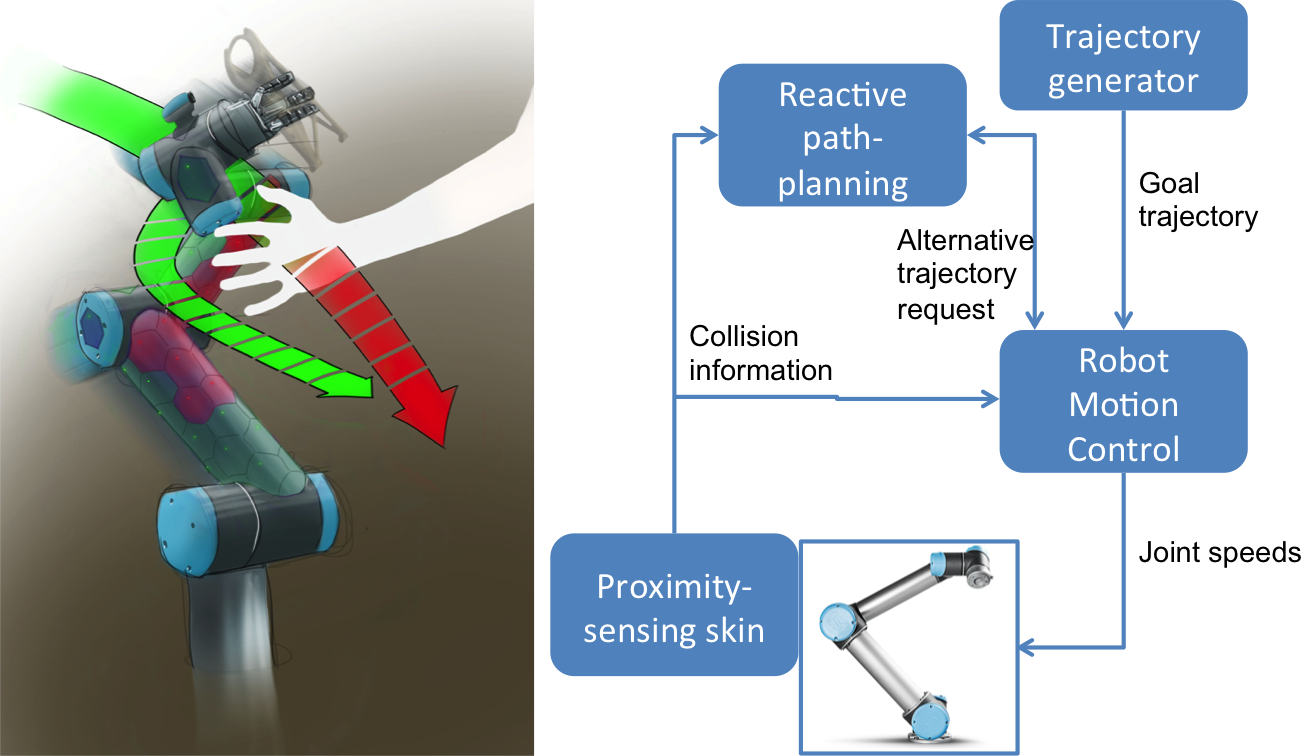
\includegraphics[scale=0.5]{chapters/doa/images/overview.png}}
\caption[0.1\textwidth]{An artist's schematization of the DOA
concept.}
\label{fig:overview}
\end{figure}
The figure \ref{fig:overview}(Left) shows the main idea of the framework which allows the robot arm to adapt its motion while executing a trajectory. The figure \ref{fig:overview}(Right) represents the pipeline of the framework used for collision avoidance and replanning. 
% \begin{figure}[h]
% \centering
% {\includegraphics[scale=1]{intro/images/gm.jpg}}
% \caption{Manufacturing unit in General Motors with 'Unimate' robots in 1969}
% \label{fig:unimate}
% \end{figure}

\begin{figure}[h]
\centering
\resizebox{0.8\columnwidth}{!}{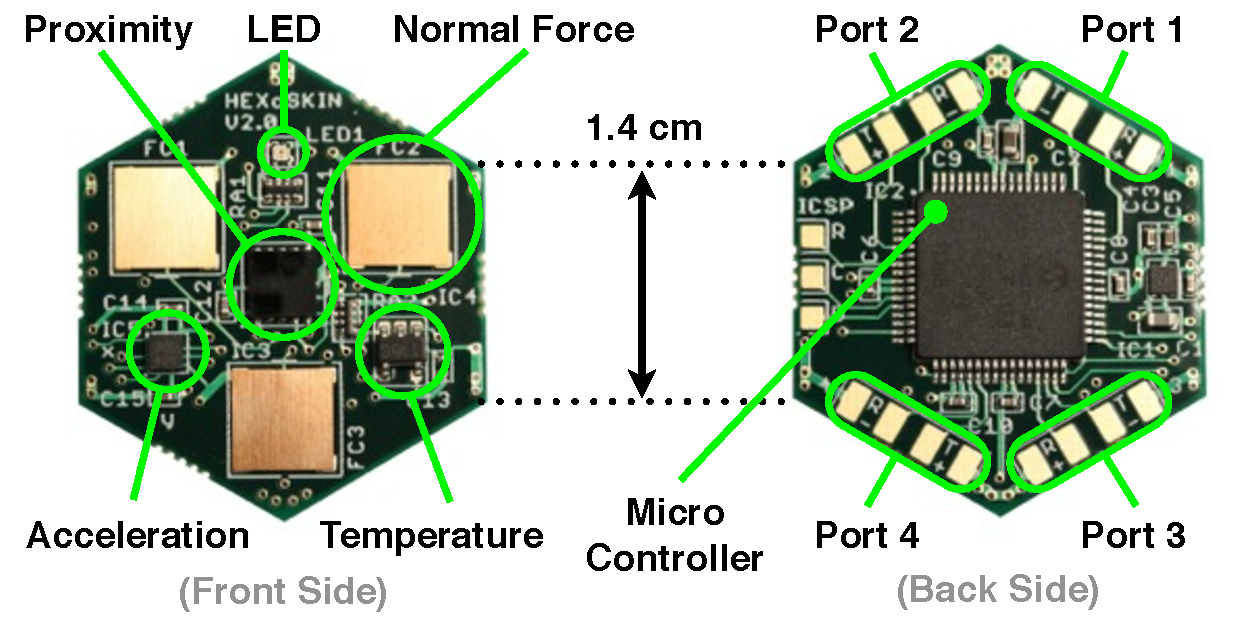
\includegraphics{chapters/doa/images/sensor_unit.pdf}}
\caption[]{Robot skin developed at Institute for Cognitive Systems, TUM.}
\label{fig:RobotSkin}
\vspace{-10pt}
\end{figure}	

\subsection{Artificial Robot Skin}
The development of \textit{Artificial Robot Skin}(ARS) is motivated by the necessity to provide robots with a rich and direct feedback of their interactions with the world. This system called as HEX-o-SKIN assembles multiple intelligent uniform unit cells with cell-2-cell communication allowing automatically cellular network organization \cite{mittendorfer2012uniform}. The robot skin system is modularized and transduces multi-modal tactile stimuli \cite{MittendorferYC15}. The robot skin consists of hexagonally shaped PCB modules called skin cells (see Fig. \ref{fig:RobotSkin}). A group of directly connected skin cells is termed skin patch. All skin cells are identical and contain the same set of sensors. The sensors sample 9 tactile stimuli of 4 different modalities, namely vibration (3D acceleration sensor), 3 normal forces (capacitive force sensor), 2 temperatures and 1 distance (optical proximity sensor). These sensors are either off-the-shelf standard ICs or in the case of the force sensors a in-house development. A micro-controller in the back of each skin cell collects data from its sensors, filters it and creates and sends data packets, which contain the most recent values of all sensors. All the skin cells are connected to each other via stretchable flex PCBs which allows the skin to cover curved surfaces and increases its robustness. The network of skin cells is a meshed bidirectional communication network which is routed by the micro-controllers of the skin cells. A self-organized algorithm initializes all the skin cells in a skin network and constructs a bidirectional communication path between each skin cell and the network root, the tactile section unit (TSU). The TSU converts skin network packets to standard UDP Ethernet packets and vice versa. This allows for fast low latency connections between robot skin and PC (see Fig. \ref{fig:SkinCellNetworkArchitecture}).
\begin{figure}[t]
\centering
\resizebox{0.8\columnwidth}{!}{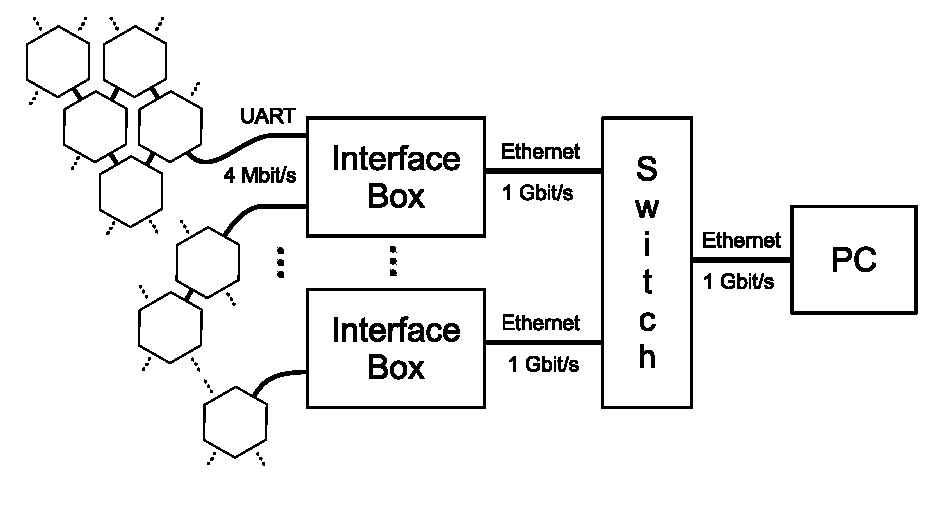
\includegraphics{chapters/doa/images/SkinCellNetwork.pdf}}\\[-15pt]
\caption[]{The skin cell network architecture and interface to the PC.}
\label{fig:SkinCellNetworkArchitecture}
\vspace{-10pt}
\end{figure}
The robot skin system also supports the auto-calibration of spatial relationships between skin cells of a skin patch covering a 3D surface \cite{Mittendorfer-IROS12tendorfer} such that the kinematic chain of every skin cell to the base frame can easily be determined. The proximity sensors used in the skin cells are infrared based sensors. The sensor emits infrared light and captures its reflections on obstacles in the range from 0 to 15 cm. The strength of the reflections allows the sensor to estimate the distance between the sensor and detected objects.  


\begin{figure}[h]
\centering
\resizebox{0.8\columnwidth}{!}{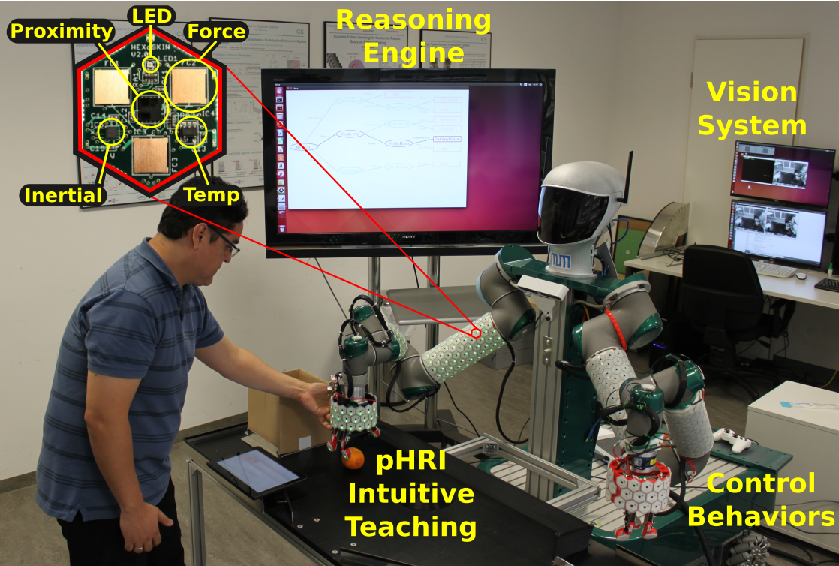
\includegraphics{chapters/doa/images/Demo.pdf}}\\[-10pt]
\caption[]{Robot TOMM with artificial robot skin.}
\label{fig:TommSorting}
\end{figure}

\paragraph{Evaluation of Artificial Robot Skin(ARS)}

The ARS has been successfully deployed on the robot TOMM \cite{Dean-ICRA17} (see Fig. \ref{fig:TommSorting}). The integration of the multi-modal artificial skin signals in the control loop of the arms is demonstrated in \cite{Dean-Humanoids16} where the self-calibrating artificial skin framework is used to control the dynamic behavior of the industrial robot, e.g. producing compliance in a non-compliant robot. The advantage of these compliant behaviors is to generate safer robots, especially for physical Human-Robot Interaction. The fusion of the multi-modal signals of the artificial skin with different sensors (e.g. cameras and joint encoders) in a semantic level is demonstrated in \cite{Ramirez-Amaro-Humanoids16}. These semantic representations are used to extract general task structures which together with the obtained knowledge can improve and accelerate teaching of new tasks \cite{Dynaov-Humanoids16}. Finally, the integration of these technologies has been evaluated in an industrial scenario, where a human can kinesthetically teach the robot TOMM to sort oranges \cite{Dean-IECON16} (see Fig. \ref{fig:TommSorting}). ARS has also been deployed successfully on another practical setup with a statically mounted Universal Robots UR5 robot (see Fig. \ref{fig:TUDSetup}). In this setup, the ARS is being used to provide proximity information related to obstacles in the immediate surroundings of the robot.

\begin{figure}[h]
\centering
\resizebox{0.8\textwidth}{!}{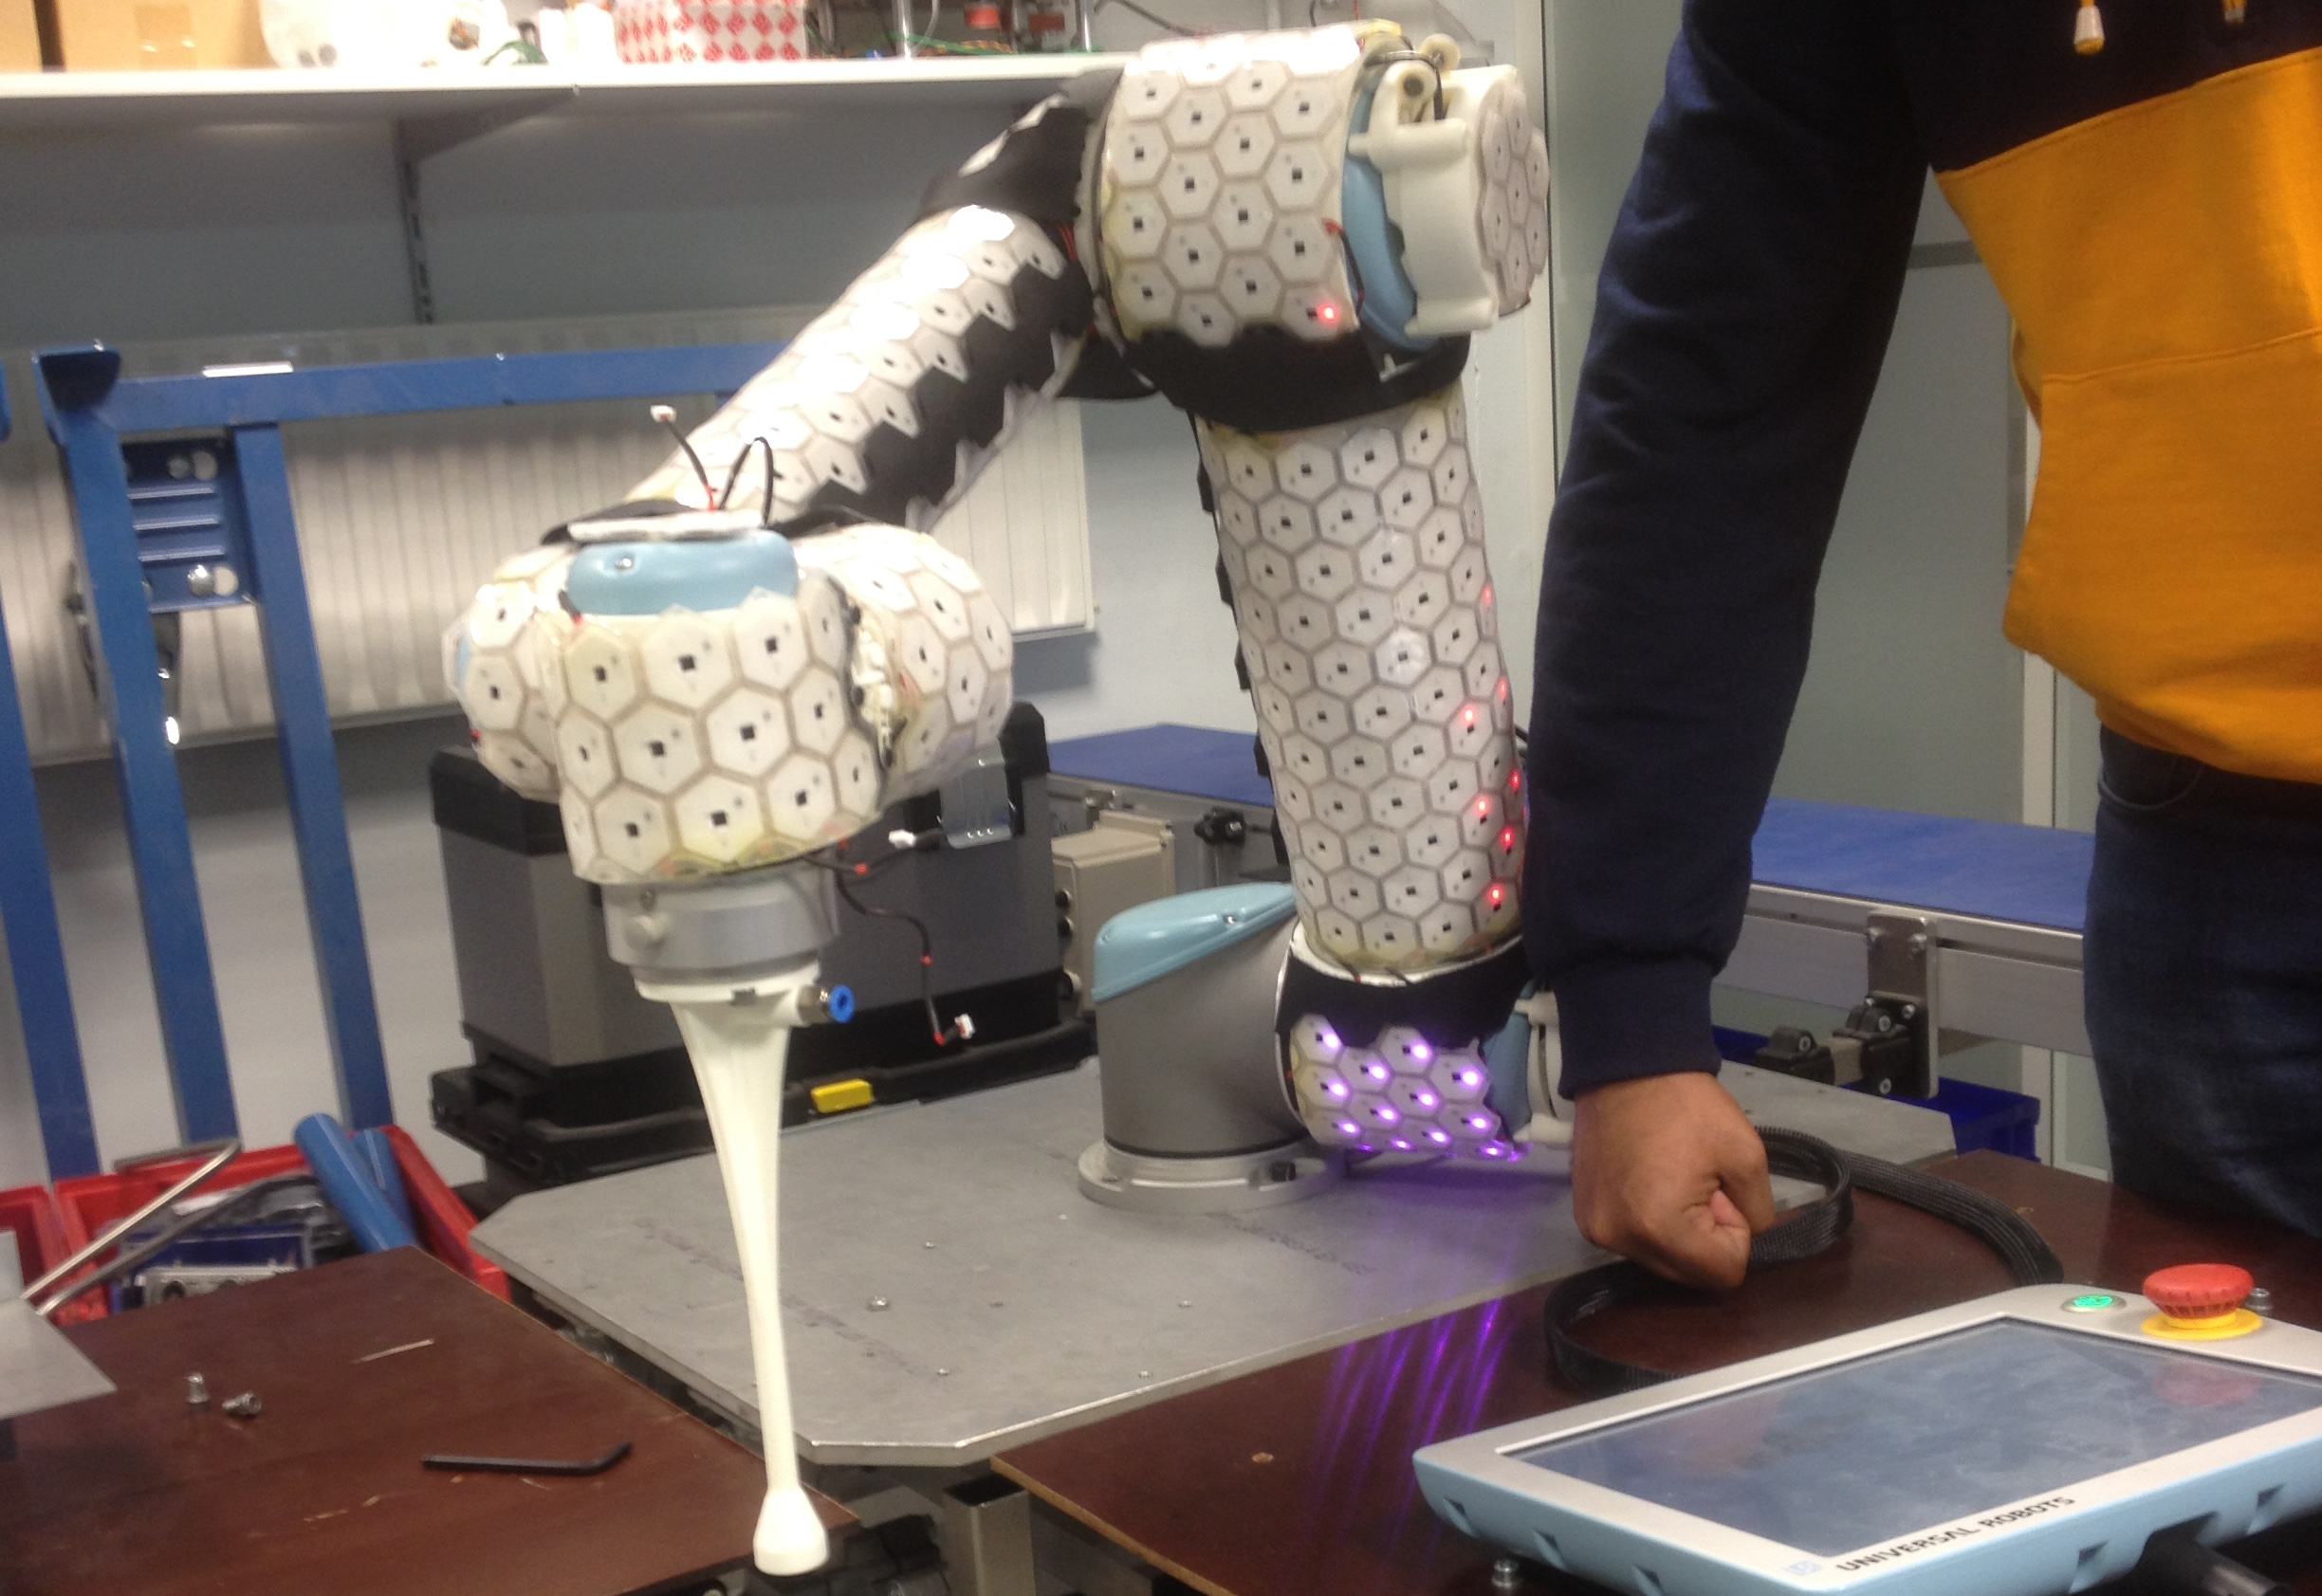
\includegraphics{chapters/doa/images/TUD_Setup.JPG}}\\[-10pt]
\caption[]{UR5 setup with Skin Cells activated (with red LEDs)}
\label{fig:TUDSetup}
\end{figure}


\subsection{Reactive Motion Planning}
\label{subsec:react_path}
\hypersetup{colorlinks, linkcolor=blue}
Though skin sensors can be used to reactively avoid obstacles locally, global aspect of the environment is necessary to avoid local minima, which is why we need an event based reactive replanner to help the controller in trouble. The reactive path planning component is developed by our partner Siemens, which is based on the industry grade KineoWorks\texttrademark\footnote{See
\href{http://www.plm.automation.siemens.com/en\_us/products/open/kineo/kineoworks/index.shtml}{Kineoworks}.} path planning library in order to provide fast and reliable robot paths. The intrinsic safety behaviors using torque/force sensing are reactive only after a collision has actually ocurred. This actually puts a constraint on the working velocity of the robot to be collaborative in industrial environments which we have pointed out earlier. The main motivation behind developing this component is to enable the robots to perform extrinsic safety behaviors which is quite inline with our goal to provide dynamic obstacle avoidance with appropriate caution. This component allows the robot to detect collisions in advance using depth information from Kinect camera and deform the trajectory by replanning in real time. The main advantage of using 3d sensors is to get a global view of the environment in contrast to proximity sensors on the surface of the robot which allows only local obstacle avoidance.

The complete collision avoidance component has been experimentally validated on a KUKA arm executing tasks in a environment with dynamic obstacles and a human operator. The reactive planner has been integrated with two trajectory generation frameworks: Reflexxes and Softmotion. Reflexxes \cite{kroger2011opening} framework can generate online time parameterized trajectories from a path. The generated jerk-limited and continuous trajectories takes into account of constraints on the dynamic robot capabilities with low latencies though there is no error bound between the reference and the executed trajectory.  The SoftMotion framework can generate online trajectories that limits jerk, acceleration and velocity for collaborative robot applications \cite{broquere2008soft,broquere2010motion}. The approach is based on the 7 segment acceleration profile by computing cubic curves for both point-point and continuous motions. The direct computation of the cubic parameters, the trajectory generator can be used on-line. Though it is incomplete as it cannot handle non-zero initial accelerations, it is experimentally validated and adapted for a KUKA LWR arm \cite{zhao2014online}. SoftMotion generates a trajectory with smoothing done at each stop point. The smoothed portion is constrained within a pre-defined tube respecting the error and kinematic bounds in real time making the trajectories more natural.



Actually, it is possible to use any trajectory generator as the planner generates a path as a polygonal line composed of a sequence of way points. For the proposed framework to avoid obstacles dynamically, we are only interested in the collision detection and the reactive planner module of this framework. The collision detection for dynamic obstacle avoidance is performed using the Kineo\texttrademark Collision Detector (KCD)\footnote{See \href{http://www.plm.automation.siemens.com/en\_us/products/open/kineo/collision-detector/index.shtml}{KCD}.}. KCD performs 3D collision detection and minimal distance analysis between triangular mesh surfaces in assembly environments. KCD has been designed specifically to minimize memory usage and take advantage of parallel processing. The component is synchronized with the OctoMap module which is updated at 30Hz with the point clouds acquired by an Xtion or Kinect camera sensors. Due to the necessity to perform reactive planning, the Octomap needs to be updated at higher rate which requires robust noise removal mechanisms. These filters removes Nan depth values and spurious points corresponding to noise, no-collision regions\& specular surfaces. The sparse outliers are removed using a statistical gaussian filter available in the PCL library \cite{rusu20113d}. The point cloud corresponding to robot links, joints and other bodies connected with the robot can be removed as well making the detection complete and flexible to be used in real time scenarios though the quality depends on a good hand-eye calibration.

\paragraph{Reactive path planning state machine}
Reactive path planning is done in the robot application node which coordinates the interaction between the path planning and the controller components executing the global tasks in real time. The path (re) planning strategy is implemented in the state machine as shown in the figure \ref{fig:KineoStates}.
\begin{itemize}
  \item \textbf{WAITING}: An idle state waiting for planning request.
  \item \textbf{PLANNING}: The controller requests the path planner node and waits for a collision free path composed of a sequence of way points. The controller executes a collision free trajectory by tracking the way points using Reflexxes or Soft Motion trajectory generator. In the proposed dynamic collision avoidance framework in the thesis, we use 'Stack of Tasks' to generate motions for a variety of reasons discussed in the next section.  In case the path planner fails due to nature of random tree algorithms, a fall back strategy to retry planning is implemented until a predefined timeout. The robot motion is cancelled in case no solutions exist.
  \item \textbf{MONITORING}: The trajectory execution by the robot is monitored for un-avoidable collisions. If the controller is intelligent enough to handle local collisions, the application node just monitors until the goal is reached. In case the obstacles doesn't allow for local path deformation, then the next state is triggered to replan.  
  \item \textbf{MONITORING WITH PLANNING PENDING}: An unavoidable collision is detected which has triggered to reach this state where the application node basically sends a new path planning request to the planner. Collisions are detected more accurately in this state as the reactive path planning considers the depth information represented in Octomap. The fast distance computation between the robot and environment using an efficient algorithm which is protected by Siemens, is used to reactively plan without creating any obstacle models which costs a lot of time.        
\end{itemize}

\begin{figure}[h]
\centering
\resizebox{1\textwidth}{!}{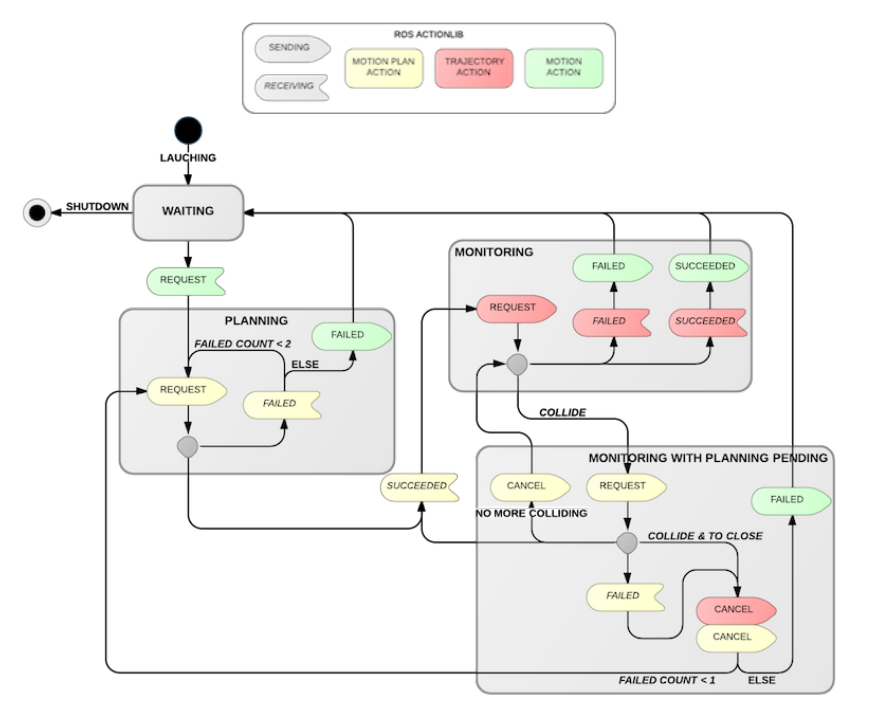
\includegraphics{chapters/doa/images/kineo_0.png}}\\[-10pt]
\caption[]{Reactive Path Planning State Machine}
\label{fig:KineoStates}
\end{figure}

This framework has been seamlessly integrated into the ROS-ecosystem via a ROS package called \texttt{kws\_ros\_interface} which provides the planner implementations of KineoWorks as shared objects that are readily usable in ROS-based software via the \texttt{kws\_ros\_planner} ROS node.Robot kinematic models are provided to KineoWorks in the Unified Robot Description Format (URDF) which is a ROS standard. Furthermore, KineoWorks also accepts the standard ROS representation of a \texttt{PointCloud}\footnote{See http://wiki.ros.org/pcl} for creating collision models of dynamic obstacles in the environment. 

\subsection{Reactive Controller}
The complete software architecture used for the Dynamic Collision Avoidance capability is shown in Fig. \ref{fig:arch_dca}. The motion control is achieved using the Stack of Tasks (SoT) controller framework \cite{Mansard2009} which employs a task based hierarchical jacobian control strategy eliminating the analytical inverse kinematics computation thus making it a generic controller for all robot platforms. 
The task function formalism is very well discussed in \cite{C.Samson1991}. A \emph{task} basically is a control law that achieves a specific objective which can be a free space task or just an inequality constraint that narrows down the workspace of the robot. The controller's hierarchical nature allows the robot to handle multiple kinematic tasks simultaneously exploiting the kinematic redundancy of the robot. The controller's real time capability comes from the high computational speed of the state of the art Hierarchical Quadratic Programming (HQP) solver backing it. In the context of our work, tasks generally include robot joint posture task, collision avoidance task, joint limits task and so on. The SoT framework handles the task priorities hierarchically in the real time to ensure there are no conflicts among tasks which is used to achieve dynamic obstacle avoidance without compromising on the main goal.

For example, let us consider a pick and place application in a collaborative environment. The primary goal for this application is to enable a robot to move to a (set of) desired pick and place locations repetitively. The pick and place locations can be defined as posture tasks in SoT. However, a higher priority task considering the collaborative nature of the environment is to avoid
collisions with obstacles that could be humans, for instance. Typically such a task is modelled as an ``Inequality'' task and an eventual feasible solution (if one exists) is computed by the solver by exploiting the kinematic redundancy of the robot. In the jargon of motion planning and control, this behavior is similar to a \emph{local planner}. However, it is likely that a feasible solution is not found due to the solver converging to a local minima\footnote{This is caused by the use of task Jacobians. For further details, please see \cite{Mansard2009}.} In such a scenario, SoT can also be used to leverage the services of a global planner (see Section \ref{subsec:react_path}) from the current robot state to the goal so that an entirely new path is obtained which is free from collisions and consequently allowing all the specified tasks to be achieved in the order of their priorities. The SoT controller has also been configured to work with the ROS-control interface. In all these setups, the proximity information from the artificial robot skin is used as an input to the collision avoidance task. In the following part, we briefly present the global path planner software framework that is used when the SoT controller hits a local minima.
\begin{figure}[t]
\centering
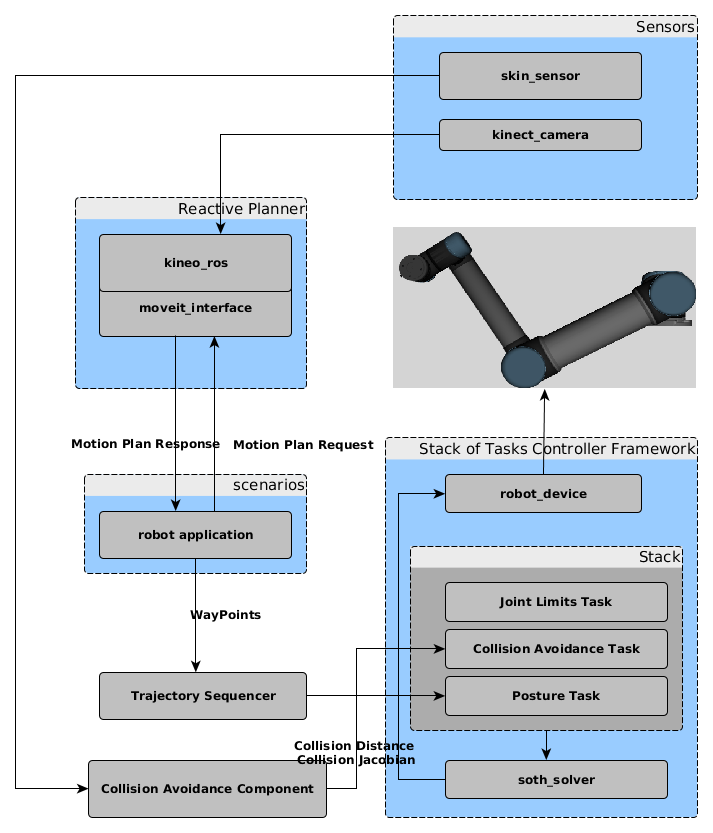
\includegraphics[scale=0.47]{chapters/doa/images/arch_dca.png}
\caption[]{Dynamic collision avoidance software architecture.}
\label{fig:arch_dca}
\end{figure}

\section{Reactive Collision Avoidance using SOT}
\label{sec:sot}
'Stack of Tasks' is a hierarchical jacobian-based task controller framework which implements the generalized inverse kinematic formalism by Hanafusa et Al. for local control of redundant systems\cite{hanafusa1981analysis}\cite{Mansard2009ik}. The framework in the earlier stages implemented the Siciliano's extension to handle multiple equality tasks\cite{siciliano1991general}. It has evolved to handle inequality constraints implementing the state of the art solver. The framework provides a structure that orders actives tasks to compute the control law without compromising on the task priority and control continuity. The framework provides a simple scripting interface to interact with controller components during the runtime and has a wrapper to communicate with the ROS world.
\subsection{State of the Art}




%    \begin{figure}[thpb]
%       \centering
%       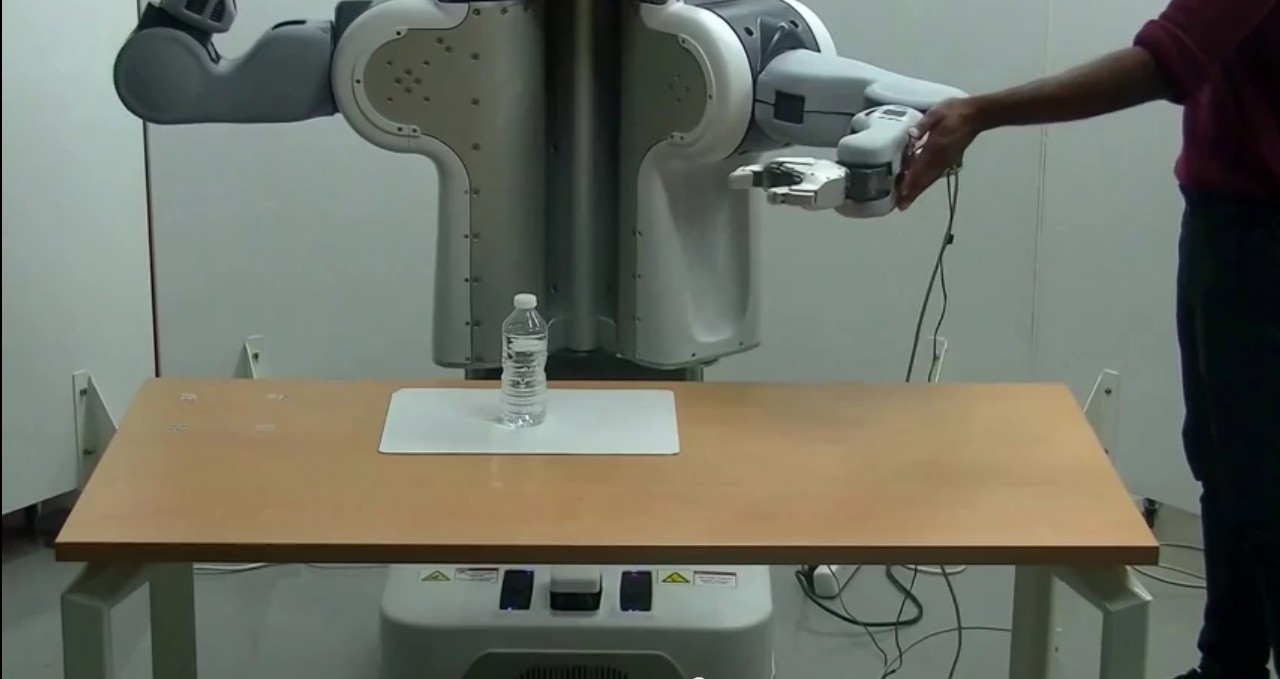
\includegraphics[scale=0.2]{chapters/doa/images/skin.eps}
%       \caption{A mobile manipulator executing a trajectory to reach a pre-grasp pose while the forearm is approached by a person with his hand. A skin sensor mounted on the forearm is used to sense any obstacle in the proximity. }
%       \label{figurelabel}
%    \end{figure}


Morover  redundant systems are popular due to their increased flexibility of arm and a mobile base to handle inequality constraints. The control of redundant robots is not trivial as it is not always easy to compute  analytic inverse kinematic and dynamic solutions. Task function based approach  resolves redundancy to minimize the error in task space \cite{Samson1991}. They are jacobian based techniques inverting the differential mapping that maps the control space and the error space to compute optimal controller outputs. A systematic framework for redundant system control proposed by Siciliano allowed to execute multiple tasks simultaneously with priorities {siciliano1991general}. These framework can only solve equality tasks and various strategies focuses on transforming inequality constraints to equalities\cite{Nelson95strategiesfor,chan1995weighted,mansard2009directional,raunhardt2007progressive}. These strategies are not generic enough and has priority inversion problems making them unreliable for practical use. 

A cascade approach was alternatively used to represent the inequalities and equalities systematically as a hierarchical least square program[Kanoun 2011] but suffered from computational inefficiencies. Hierarchical quadratic program (HQP) solver uses complete orthogonal decomposition (COD) instead of singular value decomposition (SVD) and an improved search algorithm which makes it more efficient than available solvers \cite{escande2014hierarchical}. Though constraint based approaches are quite an efficient way to handle collisions and a flexibile way to model them, the are merely locally optimal controllers and does not provide a systematic way to escape local minima. This necessitates the support of global path planners to find the optimal path for realizing a robot task. Combining global path planning and a reliable reactive control is an essential need for deploying robots from simple to complex scenarios.

 
\subsection{What is a Task?}
A task basically composes a control law with a specific objective which can be such as reaching a desired joint position, avoiding obstacles in the environment, a visual servoing mechanism for grasping or so on. A task is mainly defined by the error between the desired and current feature, the error jacobian and the gain. These defined tasks are pushed into 'Stack of Tasks' which computes the control law for all the task objectives in an iterative manner\cite{mansard2007task}. 

\[\textit{e(t) = x\textsuperscript{*} - x }\]

where \textit{x} refers to the current state of a feature, \textit{x\textsuperscript{*}} refers to the reference feature.

\subsection{Redundancy Formalism}
Siciliano and Slotine proposed a systematic control framework to compute controller outputs for achieving multiple tasks in redundant systems from the redundancy formalism proposed by Hanafusa et al. The idea is, tasks are solved only in the null space of the higher priority tasks to avoid conflicts with them. This means, a task at any level has no effect on the tasks in the higher level as it uses only the left degrees of freedom. 

Let $(e_{1},J_{1})$ be a primary task  which is defined by  
\begin{equation} \label{eq:tf1}
\dot{e} = J\dot{q} 
\end{equation}
 \textit{J} referring to the Jacobian of the error velocity with respect to joint velocity at the current joint state.


\begin{equation} \label{eq:tf3}
\dot{q} = J_{1}^{+}\dot{e}_{1} + Pz
\end{equation}
 Where \textit{P} is the projector on the null space of the the Jacobian J and \textit{ $z$ } is the arbitrary velocity vector which can be used as a parameter to achieve the secondary objectives. 

Let $(e_{1},J_{1})(e_{2},J_{2})...(e_{n},J_{n})$ be tasks in the stack. The redundancy formalism for two tasks can be extended to n tasks such that $e_{i}$ does not conflict with $e_{j}$ such that $j<i$. 


The recursive joint velocity is of the form
\begin{equation} \label{eq:ntasks}
  \dot{q}_{0} = 0\\
\end{equation}
\begin{equation}
  \dot{q}_{i} = \dot{q}_{i-1}+ (J_{i}P^{A}_{i-1})^{+}(\dot{e}_{i} - J_{i}\dot{q}_{i-1}), i= 1..n
\end{equation}



 where $P^{A}_{i-1}$ is the projector onto the null space of the augmented Jacobian $J_i^A = (J_1...J_i)$ and $\widetilde{J}_i = J_iP_{i-1}^A$ is the limited jacobian of the task. The joint velocity achieving all the task objectives is $\dot{q} = \dot{q}_n$. The recursive projector is computed by 
 
 \[P^A_i = P^A_{i-1} - (J_iP_{i-1}^A)^+J^A_{i-1}  \] 
 
 This systematic way of prioritizing tasks allows simultaneous execution of multiple tasks without conflicting each other.
 \subsection{Hierarchical Quadratic Programming}
Mansard et al. proposed an improved QP solver to manage multiple equality and inequality problems in a prioritized hierarchy to handle redundancies[15]. The solver handles equality tasks quite the same like in Siciliano's framework but the solver uses complete orthogonal decomposition(COD) instead of Sing for solving the least squares which is quite faster and efficient. The Hierarchical complete orthogonal decomposition(HCOD), a COD of the jacobian mapping for all the levels is used to compute primal optimum for all the constraints at once making it computationally faster. 

Kanoun et al. and De lasa et. al used a primal active search algorithm which is very expensive due to inefficient optimal active set search involving inappropriate activation and deactivation of constraints at each level along the cascade\cite{de2010feature}\cite{kanoun2011kinematic}. The HQP solver depends on a modified primal active search algorithm to make the optimal active set computation much more efficient. Lexicographic optimization formalism is introduced to maintain the active set at each iteration consistent with prior levels completely eliminating unnecessary constraint deactivations and activations. The solver is ten times faster than the classical solvers and can consider inequalities at any levels of the
hierarchy \cite{escande2014hierarchical}.

\subsection{Collision Avoidance using SOT}
   \begin{figure}[thpb]
      \centering
      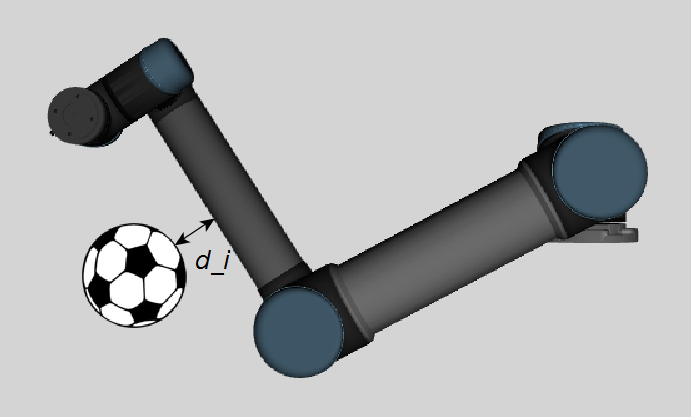
\includegraphics[scale=0.5]{chapters/doa/images/robot-obstacle_raw.png}
      \caption{Robot-Obstacle Interaction }
      \label{gso}
   \end{figure}
\subsubsection{Collision Avoidance Task Formulation}
Suppose an obstacle in the environment is close to the vicinity of the skin sensors on the robot less than a safe margin (or) threshold, the robot can move orthogonal to avoid potential collisions. Consider a multi-body robot with $n_c$ skin cells $\mathcal{C}_1,\mathcal{C}_2,\mathcal{C}_3 ... \mathcal{C}_{n_c}$ on the surface of the links. Let us also represent $\mathcal{C}_i(q)$ to be the position of the cell on the robot body  at a robot configuration q and the environment obstacle as $\mathcal{O}$. The range information from the sensors are basically the proximity distance between the skin cell and the environment obstacle in the vicinity represented by $d_i(q)$ at a robot configuration q. The below formulation is an alternative to potential field which is as follows:   
\begin{equation} \label{eq:d_ineq} 
d_i(q)  >= d_{min}
\end{equation}

Refactoring:
\[ (d_{min} - d_i(q))  <= 0\] 
\begin{equation} \label{eq:d_ineq} 
f_i(q)  <= 0
\end{equation} 

where $ f_i(q) = (d_{min} - d_i(q))$
\newline
We model an Ordinary differential inequality for the distance inequality constraint to use it in the SOT solver working in the kinematic level. 

\begin{equation} \label{eq:dd_ineq} 
\frac{\partial f_i(q) }{\partial q} \dot{q} <= - K f_i(q)
\end{equation} 

where: K is the convergence gain\newline
This formulation allows for an exponential convergence of the modeled inequality task. In our case after refactoring, \ref{eq:dd_ineq} zeros down to below form

\begin{equation} \label{eq:solver} 
-\frac{\partial d_i(q) }{\partial q}  \dot{q} <= -K (d_{min} - d_i(q))
\end{equation} 

\begin{equation} \label{eq:final} 
\dot{d_i(q)} >= K (d_{min} - d_i(q))
\end{equation}
\subsubsection{Proximity Distance Gradient Computation}
The computation of the gradient of the proximity distance between the collision bodies inspired from \cite{lefebvre2005fast} is required to define inequality constraints in Stack of Tasks to avoid self-collision and with external obstacles using a proximity sensor.

\begin{equation} \label{eq:proxd}
d_i(q) = d(\mathcal{C}_{i}(q),\mathcal{O}) = \|\mathcal{O} - \mathcal{C}_{i}(q) \|
\end{equation}
The gradient of the above distance with respect to the robot configuration is given by:

\[ \frac{\partial d_i(q) }{\partial q} = n.(\frac{\partial \mathcal{O}(q) }{\partial q}-\frac{\partial \mathcal{C}_{i}(q) }{\partial q}) \] 

where: 
\[ n = \frac{(\mathcal{O} - \mathcal{C}_{i}(q))^T}{ \|\mathcal{O} - \mathcal{C}_{i}(q) \| }\]

Assuming the environmental obstacle to be static because of the inability to measure the differential change, the gradient boils down to the below form.

\begin{equation} \label{eq:proxdiff} 
\frac{\partial d_i(q) }{\partial q} = -n.\frac{\partial \mathcal{C}_{i}(q) }{\partial q}
\end{equation}

 







% \subsection{Proximity Distance Gradient for Collision Avoidance}
% The computation of the gradient of the proximity distance between the collision bodies inspired from \cite{lefebvre2005fast} is required to define inequality constraints in Stack of Tasks to avoid self-collision and with external obstacles using a proximity sensor. Let $d$ be the distance between approximated collision bodies $O_1(q)$ and $O_2(q)$. The distance between these bodies and its variation is mapped to joint actuations $q$. The distance gradient can be computed by:
% \[ \frac{\partial d}{\partial q} = n_d^{'}(\frac{\partial o_1(q)}{\partial q}- \frac{\partial o_2(q)}{\partial q}) \]

% where $n_d^{'}$ is the unit normal distance vector while $o_1(q)$ and $o_2(q)$ are the respective closest points. The gradient of the closest point $p$ of fixed coordinates $(\rho_1(q),\rho_2(q)....\rho_l(q))$ in the local reference frame $(e_1(q),e_2(q)...,e_l(q))$ of a collision object at joint configuration $q$ is

% \[\frac{\partial p}{\partial q} =  \sum_{l=1}^{d}\rho_l(q)\frac{\partial e_l(q) }{\partial q}\]

% In a 3 dimensional workspace, the expression can be written as 

% \[ \frac{\partial p}{\partial q} =  (x y  z)J_\omega + J_\nu \]

% where $J_\omega$ is the jacobian of the rotational degrees of freedom $J_\nu$ is the jacobian of the linear degrees of freedom. In case of the external objects, the second part of the equation can be eliminated if the object is static. 

% This work is a direct application of the HQP solver and a first attempt to combine path planning and reactive control in a jacobian based solver framework eliminating a cumbersome architecture handling the information flow between control and planning components. Stack of Tasks, a controller framework that implements the latest HQP solver is used in this work to apply the proposed methodology. The proposed methodology is tested on PR2, a mobile manipulation platform with a skin sensor mounted on the forearm of the robot to demonstrate the collision avoidance while executing a planned trajectory without compromising the final goal of the scenario. 


% The paper is organised as follows. Section \ref{sec:application} describes the solution for dynamic obstacle avoidance and Section \ref{sec:skin} discusses the proximity-sensing robot skin. In Section \ref{sec:sot} the robot motion control architecture to incorporate the collision information as safety
% constraints to dynamically adapt the trajectory is presented. Section \ref{sec:prelim_results}
% presents the preliminary results obtained in two different robot setups. Finally, in Section \ref{sec:conclusions} we present our concluding remarks and a discussion of the current work in progress.




\paragraph{Combining Path Planning and Reactive Motion Control}

The methodology is based on defining the main goal as a workspace constraint and prioritizing between safety tasks and trajectory execution task (in joint space). The figure \ref{gso} gives an intuitive idea about the stack priority order.

   \begin{figure}[H]
      \centering
      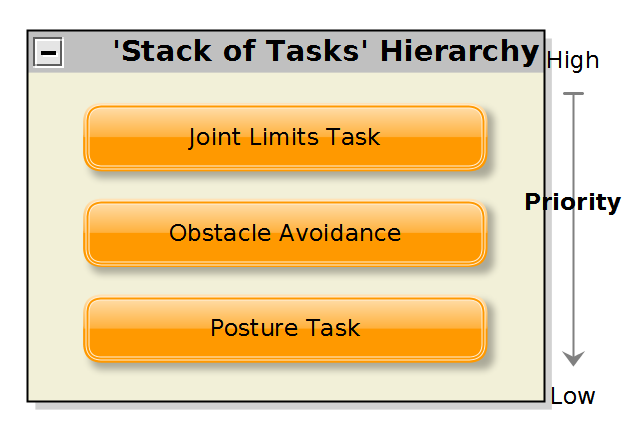
\includegraphics[scale=0.5]{chapters/doa/images/sot_hierarchy.png}
      \caption{Generic stack order for combining planning and control. }
      \label{gso}
   \end{figure}
   \begin{itemize}
  \item[T1] Obstacle Avoidance
  \newline
\hspace*{0.1cm}$\dot{d_i(q)} \geq \lambda_{1}(d_{min} - d_i(q))$\newline
\hspace*{0.11cm}where $d_{min}$ is the safety threshold
  \item[T2] Posture Task
  \newline
\hspace*{0.1cm}$\dot{q} = q_{ref} - \lambda_{2}(q-q_{ref})$\newline
\hspace*{0.1cm}where $q_{ref}$ is the reference trajectory
\end{itemize}
SOT controller computes $\dot{q}$ in order to satisfy T1 and T2 (at best)



% Safety tasks are obviously given higher priority in the stack for collision avoidance. Trajectory execution in Joint space occupies the least priority which leaves the controller only the left degrees of freedom from the primary task. If a joint trajectory crosses an unforeseen or dynamic obstacle and if the sensors can sense it, the robot basically cannot execute the trajectory until the object is actually moved out of its way. Replanning could be activated if there is no other possibility to reach the joint trajectory goal. Even if there is a possibility to avoid the obstacle and continue executing the trajectory, it is always not sure that the robot will end up in the desired goal in the task space. The clever trick here is in the way the main goals are defined. The main goal can be moving a base to a particular pose in the world or move the end effector to a grasping pose. Here the important thing is that the goals are something defined in the workspace though a joint trajectory is executed to achieve them. The hierarchical nature of the controller puts this main goal task in high priority and the jacobian core of the solver finds an optimal solution to follow the main goal. The next section illustrates this methodology on a simple scenario to show the potential of this method.



\section{Experimental verification of Reactive Collision Avoidance}
The Stack of Tasks (SoT) controller with collision avoidance constraints has also been deployed and tested for achieving different postures on the setup in Fig. \ref{fig:TUDSetup}. We have integrated the behavior to path following with the reactive collision avoidance as shown in Fig. \ref{fig:dca}. Though it is integrated, we consider these presented results preliminary yet quite convincing to be go in this direction to develop a reactive collision avoidance technology.

\subsection{Experiments in a mobile robot - PR2{\color{red}  (to be updated)}}

The framework was very initially tested with the given skin cell prototype on PR2, a mobile robot. The skin patch with eight cells is stuck on the arm to sense proximity range information. A simple manipulation scenario is executed and getting close to the arm sensors induced base motion to avoid obstacles while still executing the trajectory. The experiment can be seen here in this \href{https://youtu.be/y-6Oyi21ioQ}{\textcolor{blue}{video}} and the snapshots are shown in this Fig \ref{fig:pr2avoid}. The graph \ref{fig:basegraph} shows the evolution of the robot base when it encounters an obstacle. The safe region is where the skin cell - obstacle distance is within the right limits ensuring safety. Although the base goes away from the obstacle, it recovers back to its previous or commanded pose in the trajectory. 
\begin{figure}[ht]
\centering
\begin{subfigure}
[Getting close to the arm]{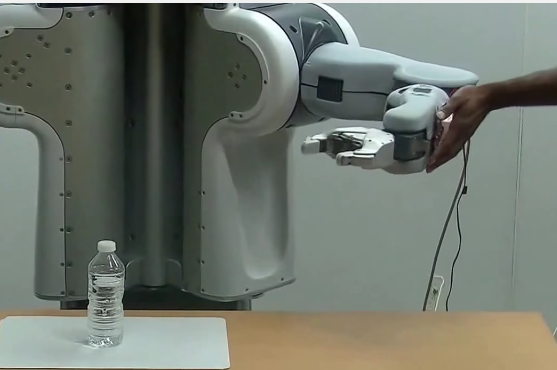
\includegraphics[width=5.5cm,height=6cm]{chapters/doa/images/pr2_0.png}}
\end{subfigure}
\begin{subfigure}
[Base motion to avoid the obstacle]{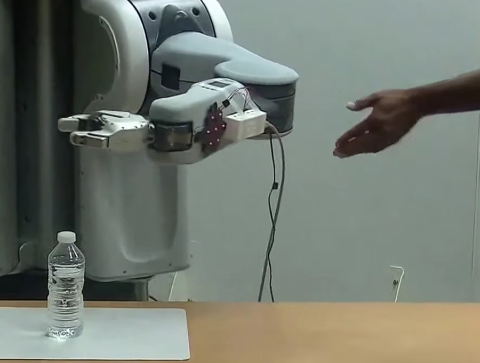
\includegraphics[width=5.5cm,height=6cm]{chapters/doa/images/pr2_1.png}}
\end{subfigure}
\caption{Obstacle Avoidance in PR2 using skin prototype}
\label{fig:pr2avoid}
\end{figure}

\begin{figure}[!ht]
\centering
{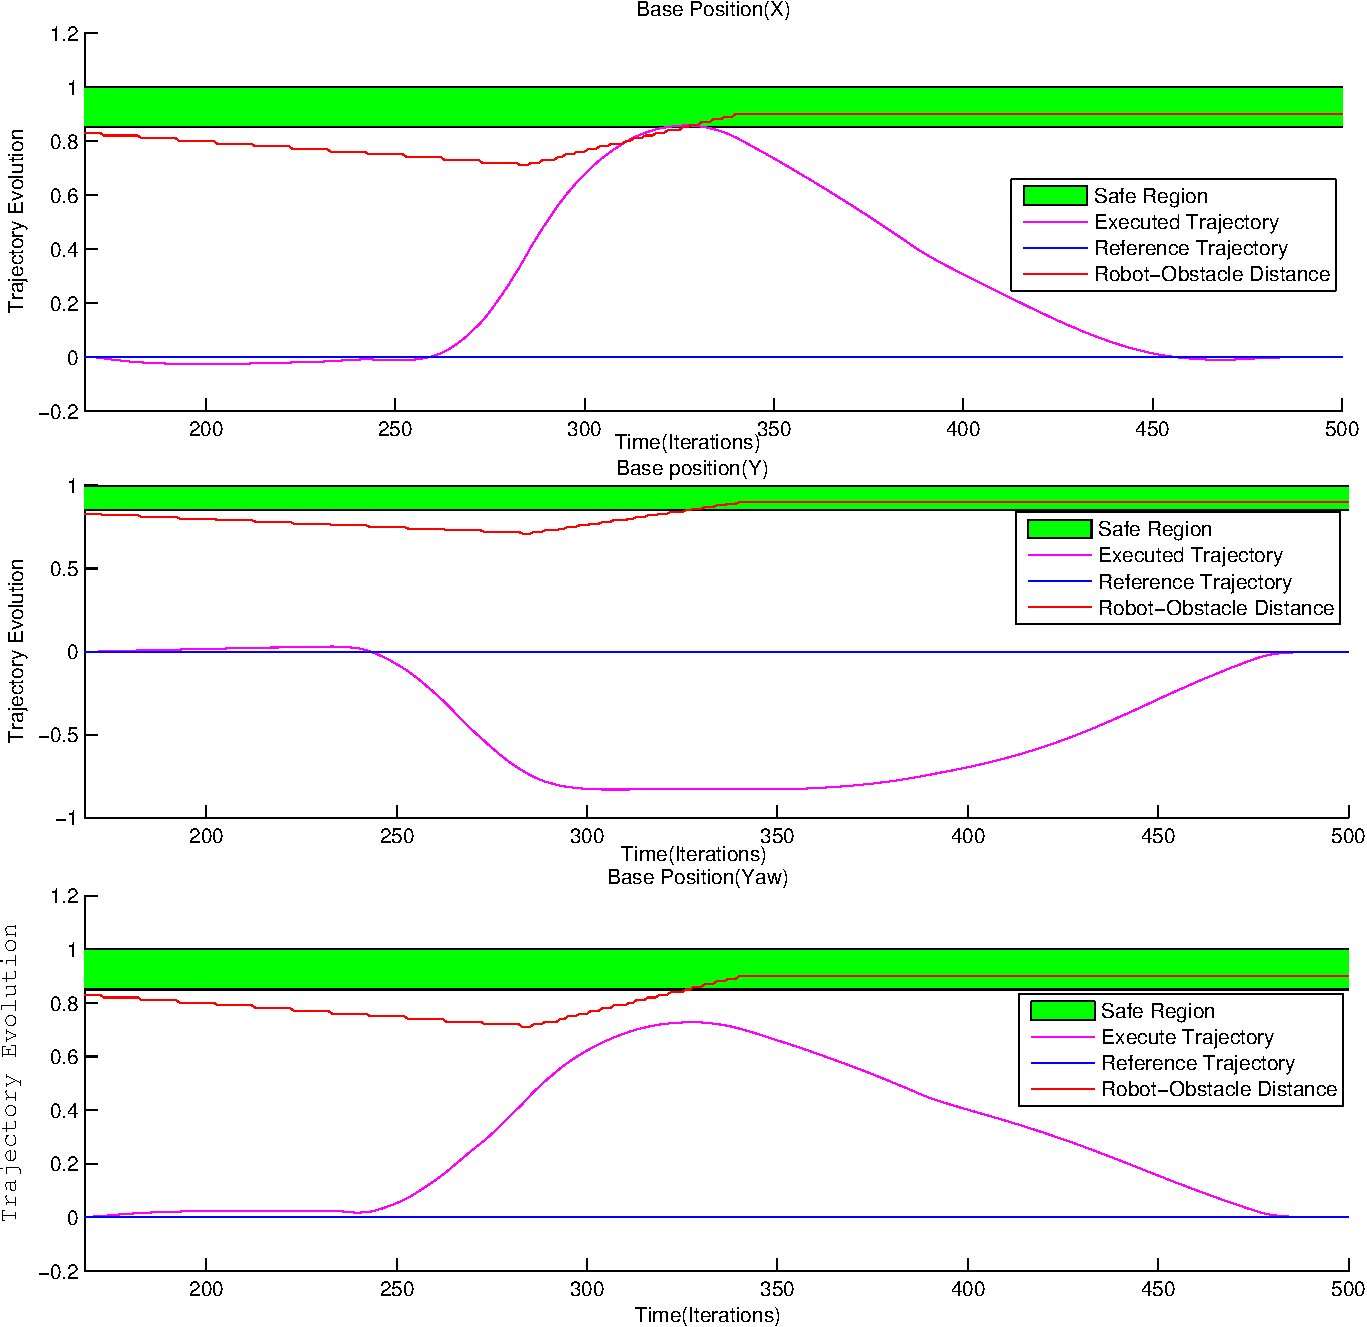
\includegraphics[scale=0.5]{chapters/doa/images/baseplot-crop.pdf}}
\caption{Base Position Evolution}
\label{fig:basegraph}
\end{figure}




\subsection{Experiments with Reactive Replanning in TOMM Setup}
\hypersetup{colorlinks, linkcolor=blue}
The integration of all the components described earlier has been evaluated on a simulation of the orange sorting setup as shown in Fig. \ref{fig:TOMMSimulation}. The evaluation is done in a ROS based gazebo environment with the skin sensors simulated using the flexible collision library to project the distance between objects to sensor range measurements. These measurements are mapped to signals compatible in dynamic graph framework using a bridge component to allow its use in the SoT controller. The reactive planning component having the capability to plan with point cloud data using a Moveit python interface to query motion plan requests. 
\begin{figure}[ht]
\centering
\resizebox{0.85\columnwidth}{!}{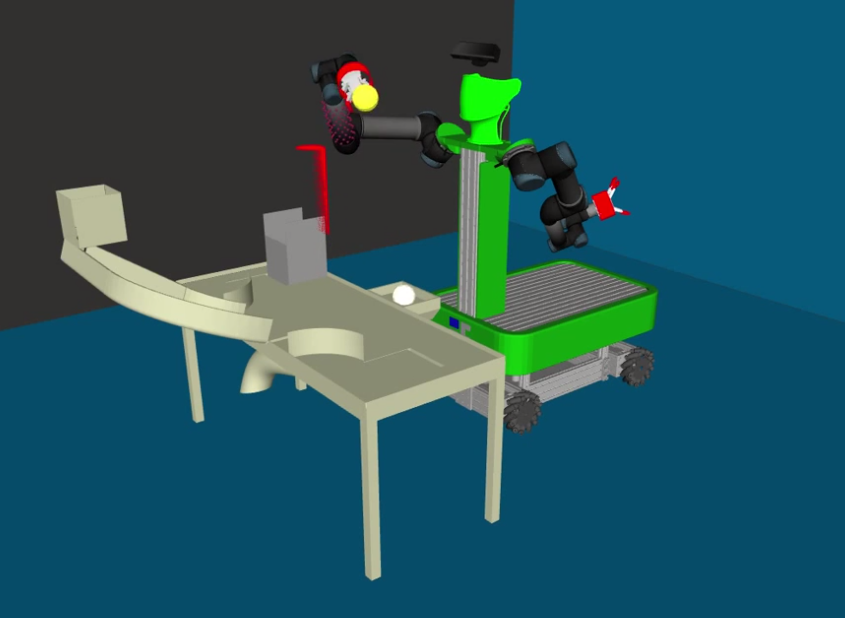
\includegraphics{chapters/doa/images/tomm_simulation.png}}\\[-10pt]
\caption[]{Orange sorting scenario in simulation.}
\label{fig:TOMMSimulation}
\end{figure}
The combined use of a reactive motion planner and a hierarchical reactive SoT controller with skin data makes it a good candidate for applying dynamical obstacle avoidance in factory environments. A video result of the same is available \href{https://youtu.be/uLStjR7mpOI}{\textcolor{blue}{here}}. Though it is tested in simulation, an experimental verification on a real robot setup with 3d cameras is quite essential to qualify the proposed framework as a promising technology. But the collision avoidance is tested on a UR robot with skin sensors to verify the local reactivity of the controller. 

\subsection{Experiments in a UR5 robot}

\begin{figure}[H]
\centering
{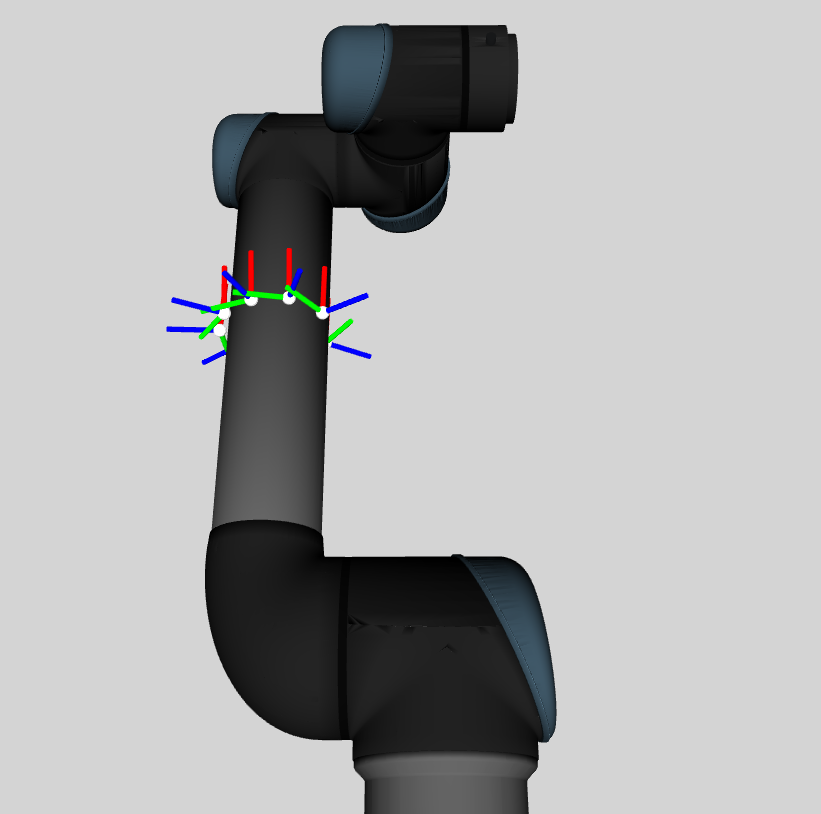
\includegraphics[width=6.5cm,height=6cm]{chapters/doa/images/delft/ring_sensors.png}}
\caption{Sensor Ring on the Upper Arm}
\label{fig:ringsensors}
\end{figure}

The reactive collision avoidance is experimentally verified on the UR5 robot with the skin sensor setup. The skin sensor network  consists of approximately 300 cells in total covering the entire surface of the UR5 robot arm. Though it is interesting to model all the skin cell constraints to be resolved by the controller, it is practically impossible to solve all the inequality constraints using the current state of the art solver due to computational constraints. A proper approximation is necessary to minimize the number of inequality constraints fed to the solver at every control cycle. In the set of preliminary experiments conducted, we defined a skin sensor ring in the upper arm as shown the figure \ref{fig:ringsensors} and collision avoidance constraints are applied only on this ring. The ring's central location on the arm gives symmetry which allows to sense information from all the directions. Another note is that the reactive replanning component is not tested in these experiments because of practical unavailability of the physical setup. 

Predefined trajectories are executed for different obstacle positions with and without collision avoidance task to verify the validity of the collision avoidance mechanism implemented. Three robot positions are chosen: Home position, Pick position and Place position. The repetitiveness of these tests on different object locations is to justify the symmetry of the ring and the robustness of the controller. There is also a complete manipulation scenario shown in the end of experiments to illustrate the practical use of the implementation. This component was successfully integrated in the final project demonstration of Factory-in-a-day which ran for more than 20 minutes robustly without any controller failure though it is possible in the most optimization based solvers. The simplicity of the approach and the practical relevance makes it a best candidate for being used in industries. 

\begin{figure}[H]
\centering
\begin{subfigure}
[Home Position]{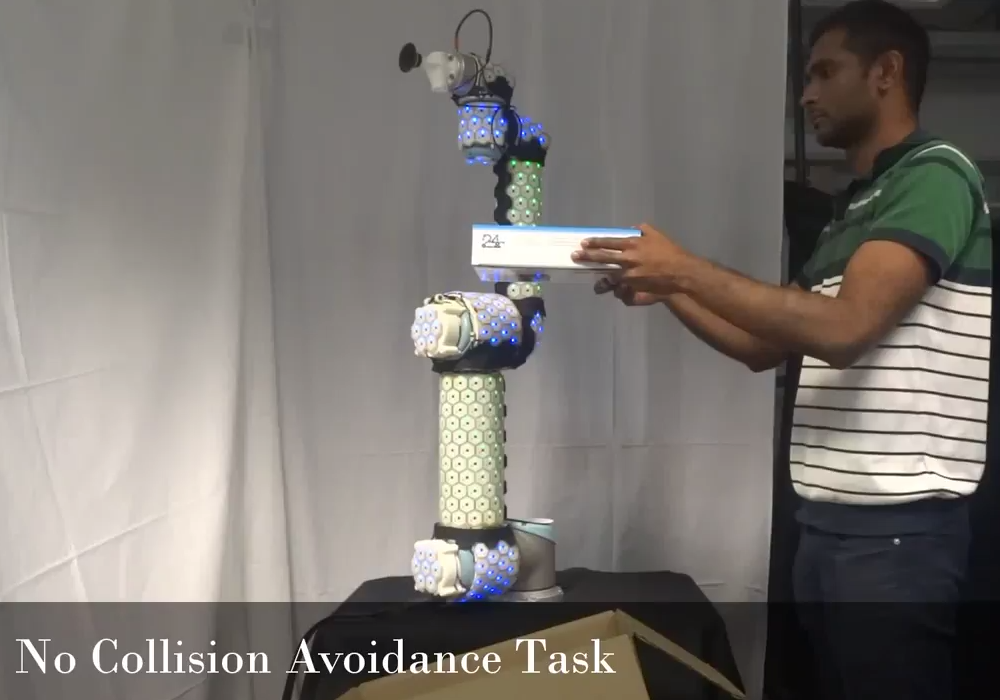
\includegraphics[width=6.5cm,height=6cm]{chapters/doa/images/delft/test_home2pick/cropped/test0_0-cropped.png}}
\end{subfigure}
\begin{subfigure}
[Colliding with Obstacle]{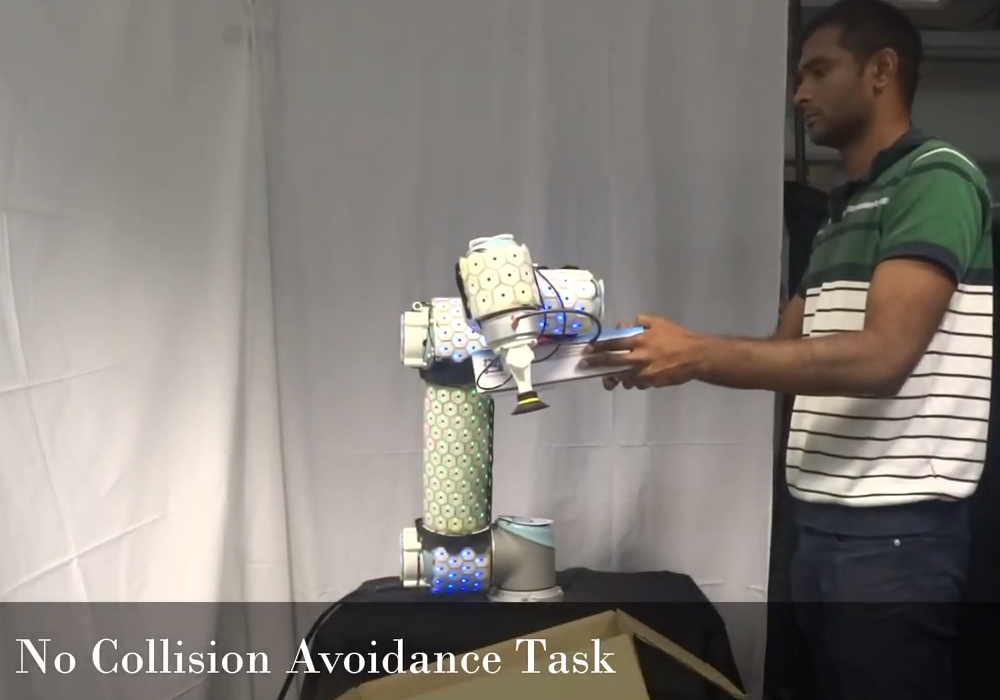
\includegraphics[width=6.5cm,height=6cm]{chapters/doa/images/delft/test_home2pick/cropped/test0_1-cropped.png}}
\end{subfigure}
\begin{subfigure}
[Avoiding Local Collisions]{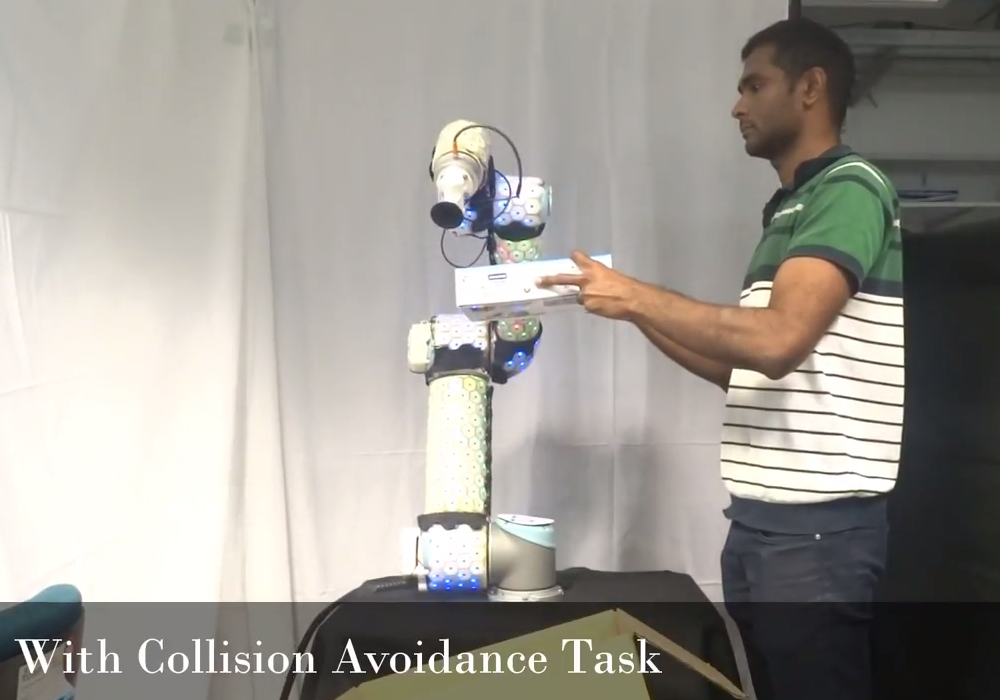
\includegraphics[width=6.5cm,height=6cm]{chapters/doa/images/delft/test_home2pick/cropped/test0_2-cropped.png}}
\end{subfigure}
\begin{subfigure}
[Place Position after avoiding Collisions]{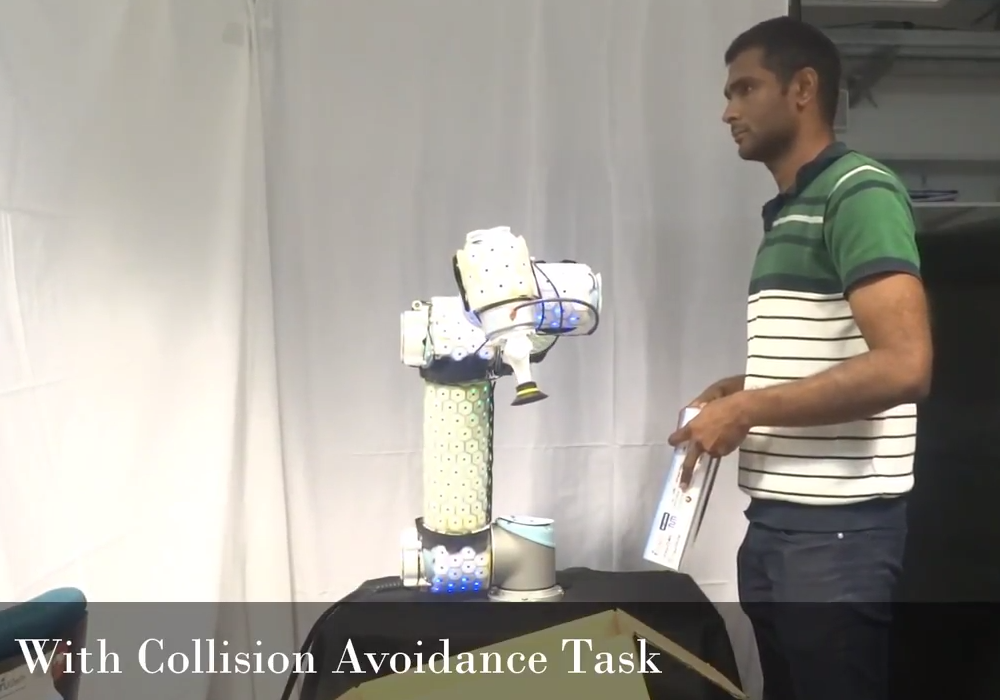
\includegraphics[width=6.5cm,height=6cm]{chapters/doa/images/delft/test_home2pick/cropped/test0_3-cropped.png}}
\end{subfigure}
\caption{Test 1: Trajectory execution from home to pick location with and without collision avoidance task in the controller stack. (b) shows the collision with the obstacle without the ability to avoid collision. (b) shows the collision avoidance of the arm though it gets stuck in the local minima but reaches the goal after the obstacle is removed.}
\label{fig:h2ptest1}
\end{figure}
The experimental validation done on the robot can be seen in these videos demonstrating three scenarios : \href{https://goo.gl/LVbQZz}{\textcolor{blue}{home to pick}}, \href{https://goo.gl/7jCqzA}{\textcolor{blue}{pick to place}}, \href{https://goo.gl/GP8KAA}{\textcolor{blue}{place to home}}. As it can be seen, a box is used as an obstacle to interrupt the executed path. Three tests are conducted at different obstacle locations introducing variability in the environment with these obstacles. Though there are many tests conducted, let us focus on certain tests and the behavior to illustrate the performance of the controller. The figure \ref{fig:h2ptest1} shows the test executing a trajectory from home to pick location with a fixed obstacle location as shown. (a) shows the initial state of the robot which is the home position and (b) shows the trajectory execution without any collision avoidance task to differentiate with the behavior generated by the controller with collision avoidance task. The robot evading collisions and its inability to reach the goal because of the object can be seen in (c) and (d). It gets stuck in local minima but manages to reach the goal after the object is removed. 

\begin{figure}[H]
\centering
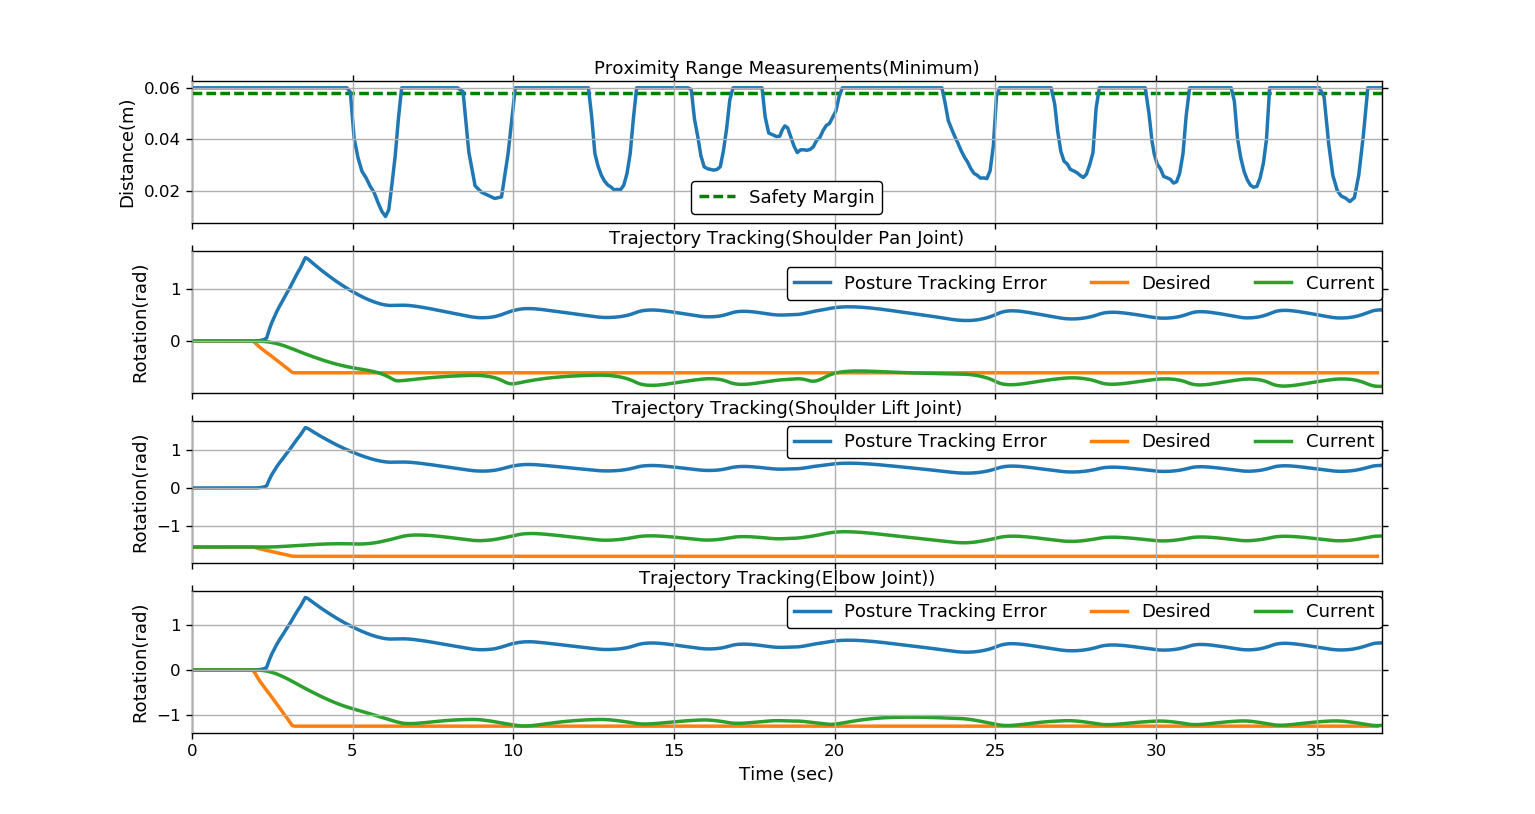
\includegraphics[width=18cm,height=13cm,center]{chapters/doa/images/delft/test_home2pick/plot_0.png}
\caption{Test 1: Plot during a Home to Pick Trajectory Execution: (1) shows the the min of range measurements from 8 skin sensor cells showing the vicinity of obstacles to the upper arm. (2),(3) and (4) shows the disturbances in the trajectory tracking when an obstacle is in the vicinity. The Posture tracking error doesn't settle to zero because of the local minima it encounters, resulting in continuous oscillations trying to go across the obstacle with a hope the obstacle will move away'}
\label{Home2Pick:test1}
\end{figure}
The plot in \ref{Home2Pick:test1}, \ref{Home2Pick:test2} shows the evolution of the trajectory tracking error and the proximity range measurements during the execution of a trajectory from home to pick with two obstacle locations respectively. The minimum of the proximity measurements of 8 cells is taken to show in the plots showing the presence of the obstacle close to the arm. The trajectory tracking error is the 2-norm of the current state of the robot and the posture command of the trajectory sequencer fed to posture task stacked in the solver.  Along with the trajectory error, the three major joints: shoulder pan, shoulder lift and the elbow joint states are plotted with the desired state to show the perturbations in response to the obstacle close to the arm. In both the plots, it can be observed that the trajectory tracking error increases rapidly irrespective of the obstacles at a proximity distance above the safety margin. This is because of the formulation as shown in \ref{eq:dd_ineq}, the collision avoidance task constrains the velocity of the skin cell based on the difference between the safety margin and the measured range. From the plots it can be observed, the difference is around 2 millimeter when there is no object close to the arm. The skin sensor range information is saturated to 6cm as the measurements above 6cm are highly nonlinear and unreliable. The 2mm difference along with smaller task gains reduces the speed of the robot. Though the saturation value can be adjusted to improve the speed of the robot behavior, the plots correspond to a non-ideal setting but still shows a robust collision avoidance. 


\begin{figure}[H]
\centering
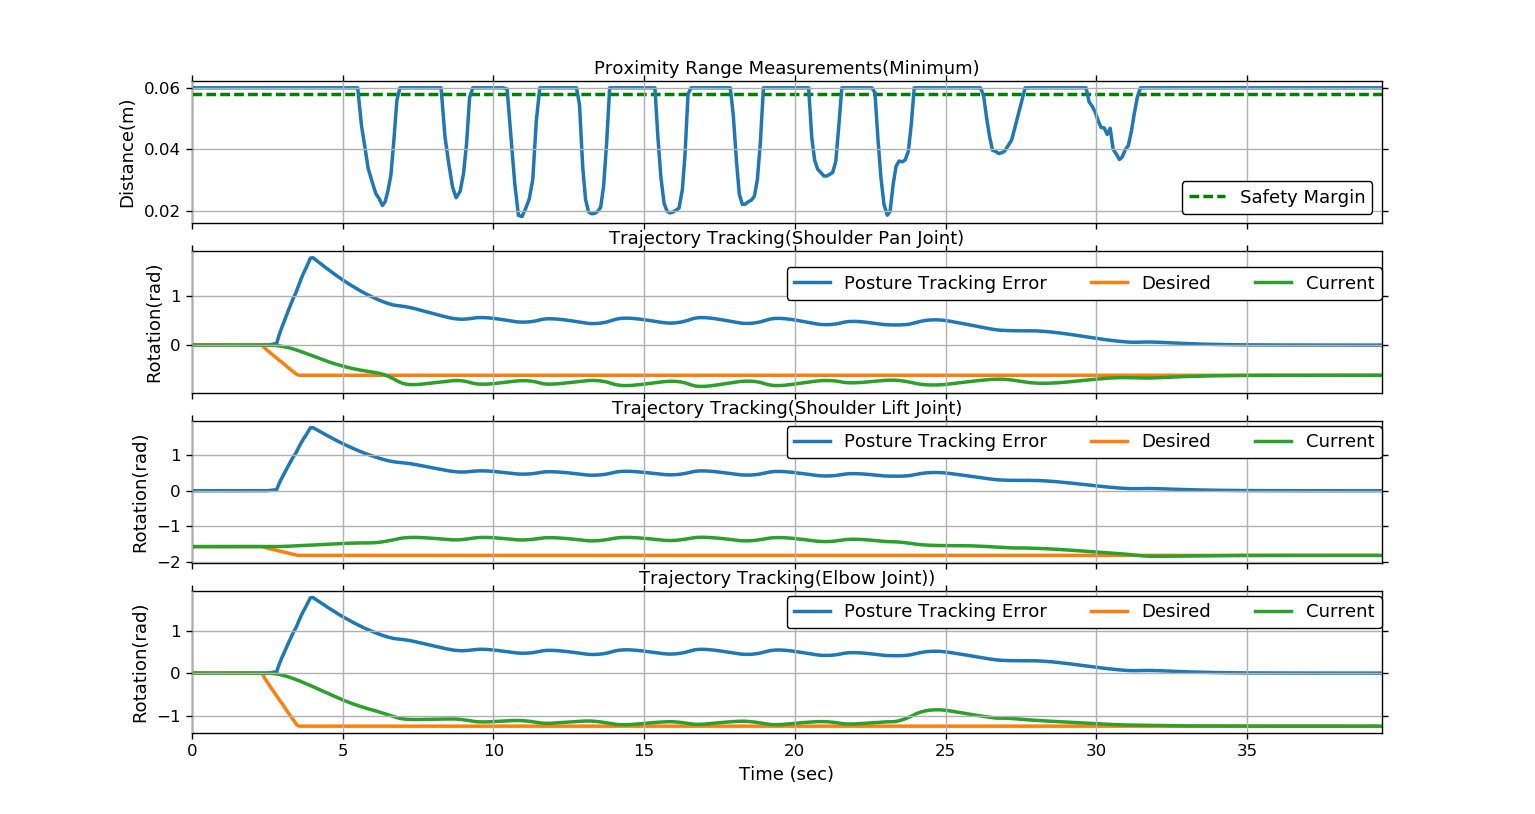
\includegraphics[width=18cm,height=13cm,center]{chapters/doa/images/delft/test_home2pick/plot_1.png}
\caption{Test 2: Plot during a Home to Pick Trajectory Execution: (1) shows the the min of range measurements from 8 skin sensor cells showing the vicinity of obstacles to the upper arm. (2),(3) and (4) shows the disturbances in the trajectory tracking when an obstacle is in the vicinity. The Posture tracking error settles to zero because the resulting deformation in trajectory was sufficient to evade obstacles and still achieve the goal.}
\label{Home2Pick:test2}
\end{figure}

In both the plots \ref{Home2Pick:test1} and \ref{Home2Pick:test2} , the disturbances in trajectory tracking when an obstacle is in the vicinity. In \ref{Home2Pick:test1}, the posture tracking error doesn’t settle to zero because of the local minima it encounters, resulting in continuous oscillations trying to go across the obstacle with a hope the obstacle will move away. In \ref{Home2Pick:test1}, the posture tracking error settles to zero because the resulting deformation in trajectory was sufficient to evade obstacles and still achieve the goal. In contrast to the previous plots, the plot \ref{Home2Pick:nocollision} shows the trajectory execution without collision avoidance task in the stack. As it can be seen in the video and in the plot, the trajectory execution was not affected while the arm literally goes across the obstacles which can be seen in the closeness of arm with the obstacles. The shoulder pan \& lift joint, elbow joint trajectory tracking is smooth without any disturbances like we saw in the previous plots validating the controller(with collision avoidance task) of taking actions in response to the obstacles in the vicinity.

\begin{figure}[H]
\centering
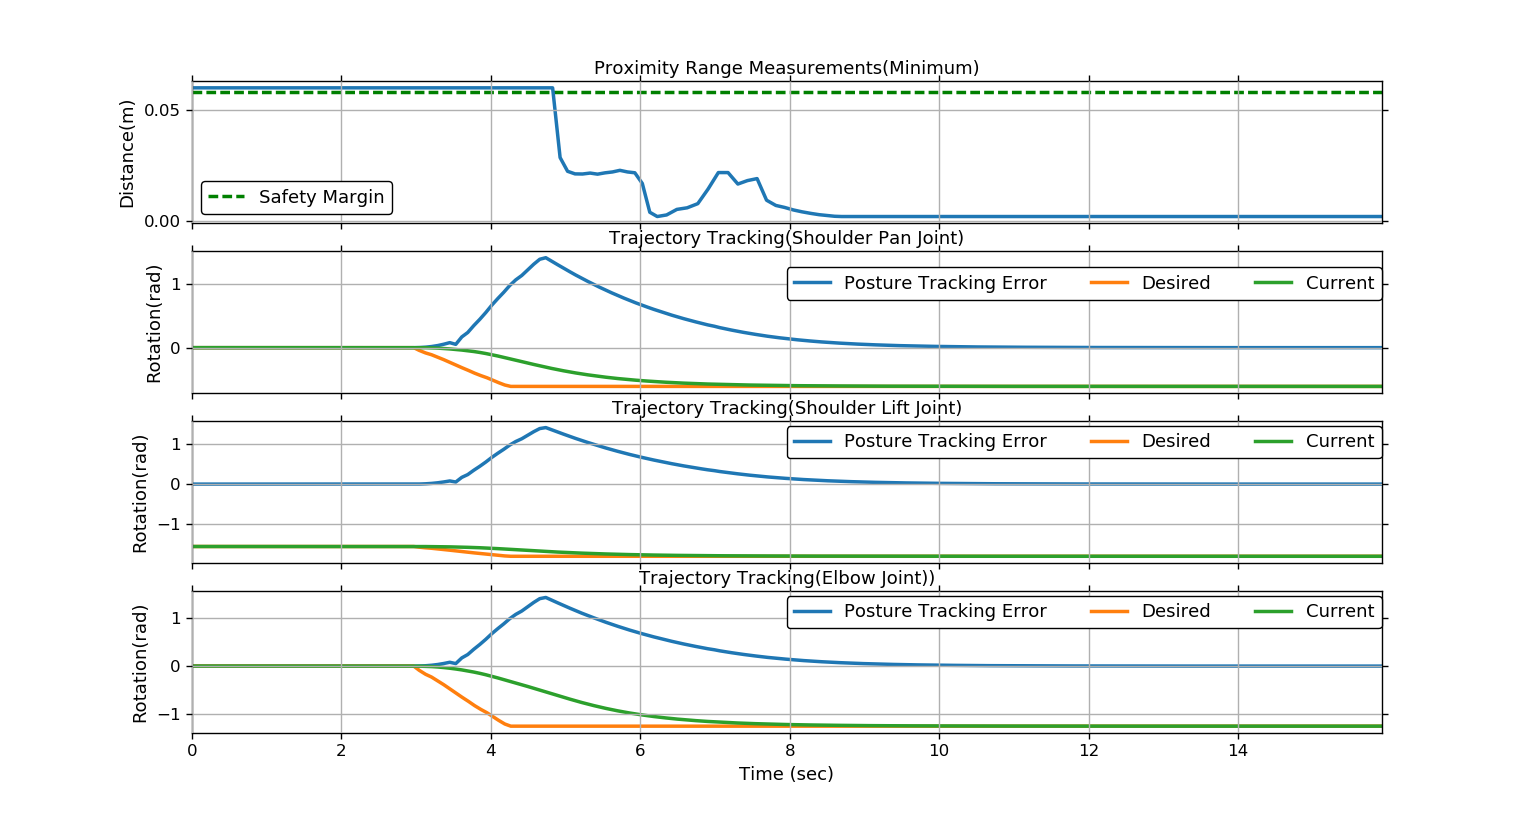
\includegraphics[width=18cm,height=13cm,center]{chapters/doa/images/delft/test_home2pick/plot_0_nocollision.png}
\caption{Test 1: Plot during a Home to Pick Trajectory Execution with no Collision Avoidance task in the Stack: (1) shows the the min of range measurements from 8 skin sensor cells showing the vicinity of obstacles to the upper arm. The sensor range drops close to zero showing the obstacle literally touching the robot. (2),(3) and (4) shows no disturbances in the trajectory tracking when an obstacle is in the vicinity. The Posture tracking error settles to zero after reaching the goal just by hitting the obstacle obviously because of no awareness.}
\label{Home2Pick:nocollision}
\end{figure}

The figure \ref{fig:p2ptest3} shows the test executing a trajectory from pick to place location with a fixed obstacle location as shown. (a) shows the initial state of the robot which is the pick position and (b) shows the trajectory execution without any collision avoidance task to differentiate with the behavior generated by the controller with collision avoidance task. The robot evading collisions and its ability to reach the goal by deforming the trajectory as seen in (c),(d) and (e) to reach (f). Similar natural behaviors can be seen in the rest of the videos referred previously.

\begin{figure}[H]
\centering
\begin{subfigure}
[Initial State - Pick Position]{\includegraphics[width=6.5cm,height=6cm]{chapters/doa/images/delft/test_pick2place/cropped/test2_0-cropped.png}}
\end{subfigure}
\begin{subfigure}
[Colliding with Obstacle]{\includegraphics[width=6.5cm,height=6cm]{chapters/doa/images/delft/test_pick2place/cropped/test2_1-cropped.png}}
\end{subfigure}
\begin{subfigure}
[Avoiding Local Collisions 1/3]{\includegraphics[width=6.5cm,height=6cm]{chapters/doa/images/delft/test_pick2place/cropped/test2_2-cropped.png}}
\end{subfigure}
\begin{subfigure}
[Avoiding Local Collisions 2/3]{\includegraphics[width=6.5cm,height=6cm]{chapters/doa/images/delft/test_pick2place/cropped/test2_2_1-cropped.png}}
\end{subfigure}
\begin{subfigure}
[Avoiding Local Collisions 3/3]{\includegraphics[width=6.5cm,height=6cm]{chapters/doa/images/delft/test_pick2place/cropped/test2_2_2-cropped.png}}
\end{subfigure}
\begin{subfigure}
[Final State - Place Position]{\includegraphics[width=6.5cm,height=6cm]{chapters/doa/images/delft/test_pick2place/cropped/test2_3-cropped.png}}
\end{subfigure}
\caption{Trajectory execution from pick to place location with and without collision avoidance task in the controller stack. (b) shows the collision with the obstacle without the ability to avoid collision. (b) shows the collision avoidance of the arm with a deformation in trajectory that allows the reach the goal with ease.}
\label{fig:p2ptest3}
\end{figure}

The reactive collision avoidance component after proper tuning is applied on a complete manipulation scenario involving multiple sequences of pick and place operations of boxes and shaving cans using a suction gripper in the end effector. The robot controller still holds the same ring of collision constraints in the upper arm for simplicity. The demonstration video is shown in this link \href{https://goo.gl/PLbKdb}{\textcolor{blue}{here}} with snapshots shown in . 

\begin{figure}[H]
\centering
\begin{subfigure}
[Grasping with a suction gripper]{\includegraphics[width=6.5cm,height=6cm]{chapters/doa/images/delft/complete/suckstill-cropped.png}}
\end{subfigure}
\begin{subfigure}
[Avoiding Obstacles]{\includegraphics[width=6.5cm,height=6cm]{chapters/doa/images/delft/complete/avoiding-cropped.png}}
\end{subfigure}
\caption{Illustrating obstacle avoidance while picking and placing small objects using a suction gripper. The full scenario video can be seen in this \href{https://goo.gl/PLbKdb}{\textcolor{blue}{video}}.}
\label{fig:final_scenario}
\end{figure}

\begin{figure}[H]
\centering
\includegraphics[width=18cm,height=8cm,center]{chapters/doa/images/delft/plot_satisfy.png}
\caption{Plot showing the evolution of a skin cell velocity satisfying the \ref{eq:dd_ineq} when the other cells have no obstacles in the vicinity.}
\label{fig:plotsatisfy}
\end{figure}

Another interesting aspect of the controller is the ability to compromise with the collision constraint inequalities in case the modeled constraint is not feasible without breaking the solver making the controller reliable. The plot \ref{fig:plotsatisfy} shows the change in velocity of a specific skin cell in response to changing obstacle in the vicinity. This plot is generated by simulating a distance signal to cell number 4 (among the 8 cells) around the safety margin while keeping the other skin cell values equal to 0.6 which is 10 times far away from the safety margin. This shows a practical feasibility of the goal thus resulting in a behavior inline with the formulated collision avoidance constraint in \ref{eq:dd_ineq}. 

But when we have a situation where the obstacles are around the arm in all directions within or beyond the safety margin, the controller compromises with the collision avoidance constraint as shown in the plot. This might look like a design issue but this is purely because of the nature of the HQP solver which compromises with the goal to achieve the maximum possible without breaking the controller or generating bad motion behaviors making it reliable. 

\begin{figure}[H]
\centering
\includegraphics[width=18cm,height=8cm,center]{chapters/doa/images/delft/plot_unsatisfy.png}
\caption{Plot showing the evolution of a skin cell velocity not satisfying the \ref{eq:dd_ineq} when the other cells have obstacles in the vicinity but not inside the safety margin. The other skin cells are simulated to measure 6cm which is just 2mm from the safety margin. This constrains the upper arm in achieving a skin cell velocity satisfying the \ref{eq:dd_ineq} as the control believes there is an obstacle still around hence resulting in safer motions.}
\label{fig:plot_unsatisfy}
\end{figure}







\section{Conclusion{\color{red}(to be updated)}}
\label{doa:conclusion}
This chapter presented the technologies that have been developed in the FiaD project to augment collaborative robot manipulators with dynamic obstacle avoidance. All these technologies: a proximity-sensing robot skin, a reactive path planning solution and a robot motion control strategy, have been validated in laboratory prototypes. Also, a preliminary prototype of an integrated solution based on these technologies has been tested in simulation. Effort on making the collision avoidance component generic enough to handle all the skin sensors by feeding only the minimal activated skin cells.  

\ifdefined\included
\else
\bibliographystyle{acm}
\bibliography{These}
\end{document}
\fi
% \ifdefined\included
\else
\documentclass[a4paper,11pt,twoside]{StyleThese}
\usepackage{amsmath,amssymb}             % AMS Math
\usepackage[T1]{fontenc}
\usepackage[utf8x]{inputenc}
\usepackage{babel}
\usepackage{datetime}

\usepackage{lmodern}
\usepackage{tabularx}
%\usepackage{tabular}
\usepackage{multirow}

\usepackage{hhline}
\usepackage[left=1.5in,right=1.3in,top=1.1in,bottom=1.1in,includefoot,includehead,headheight=13.6pt]{geometry}
\renewcommand{\baselinestretch}{1.05}

% Table of contents for each chapter

\usepackage[nottoc, notlof, notlot]{tocbibind}
\usepackage{minitoc}
\setcounter{minitocdepth}{2}
\mtcindent=15pt
% Use \minitoc where to put a table of contents

\usepackage{aecompl}

% Glossary / list of abbreviations

\usepackage[intoc]{nomencl}
\iftoggle{ThesisInEnglish}{%
\renewcommand{\nomname}{Glossary}
}{ %
\renewcommand{\nomname}{Liste des Abréviations}
}

\makenomenclature

% My pdf code

\usepackage{ifpdf}

\ifpdf
  \usepackage[pdftex]{graphicx}
  \DeclareGraphicsExtensions{.jpg}
  \usepackage[a4paper,pagebackref,hyperindex=true]{hyperref}
  \usepackage{tikz}
  \usetikzlibrary{arrows,shapes,calc}
\else
  \usepackage{graphicx}
  \DeclareGraphicsExtensions{.ps,.eps}
  \usepackage[a4paper,dvipdfm,pagebackref,hyperindex=true]{hyperref}
\fi

\graphicspath{{.}{images/}}

%% nicer backref links. NOTE: The flag ThesisInEnglish is used to define the
% language in the back references. Read more about it in These.tex

\iftoggle{ThesisInEnglish}{%
\renewcommand*{\backref}[1]{}
\renewcommand*{\backrefalt}[4]{%
\ifcase #1 %
(Not cited.)%
\or
(Cited in page~#2.)%
\else
(Cited in pages~#2.)%
\fi}
\renewcommand*{\backrefsep}{, }
\renewcommand*{\backreftwosep}{ and~}
\renewcommand*{\backreflastsep}{ and~}
}{%
\renewcommand*{\backref}[1]{}
\renewcommand*{\backrefalt}[4]{%
\ifcase #1 %
(Non cité.)%
\or
(Cité en page~#2.)%
\else
(Cité en pages~#2.)%
\fi}
\renewcommand*{\backrefsep}{, }
\renewcommand*{\backreftwosep}{ et~}
\renewcommand*{\backreflastsep}{ et~}
}

% Links in pdf
\usepackage{color}
\definecolor{linkcol}{rgb}{0,0,0.4} 
\definecolor{citecol}{rgb}{0.5,0,0} 
\definecolor{linkcol}{rgb}{0,0,0} 
\definecolor{citecol}{rgb}{0,0,0}
% Change this to change the informations included in the pdf file

\hypersetup
{
bookmarksopen=true,
pdftitle="Évaluation de la sécurité des équipements grand public connectés à Internet",
pdfauthor="Yann BACHY", %auteur du document
pdfsubject="Thèse", %sujet du document
%pdftoolbar=false, %barre d'outils non visible
pdfmenubar=true, %barre de menu visible
pdfhighlight=/O, %effet d'un clic sur un lien hypertexte
colorlinks=true, %couleurs sur les liens hypertextes
pdfpagemode=None, %aucun mode de page
pdfpagelayout=SinglePage, %ouverture en simple page
pdffitwindow=true, %pages ouvertes entierement dans toute la fenetre
linkcolor=linkcol, %couleur des liens hypertextes internes
citecolor=citecol, %couleur des liens pour les citations
urlcolor=linkcol %couleur des liens pour les url
}

% definitions.
% -------------------

\setcounter{secnumdepth}{3}
\setcounter{tocdepth}{2}

% Some useful commands and shortcut for maths:  partial derivative and stuff

\newcommand{\pd}[2]{\frac{\partial #1}{\partial #2}}
\def\abs{\operatorname{abs}}
\def\argmax{\operatornamewithlimits{arg\,max}}
\def\argmin{\operatornamewithlimits{arg\,min}}
\def\diag{\operatorname{Diag}}
\newcommand{\eqRef}[1]{(\ref{#1})}

\usepackage{rotating}                    % Sideways of figures & tables
%\usepackage{bibunits}
%\usepackage[sectionbib]{chapterbib}          % Cross-reference package (Natural BiB)
%\usepackage{natbib}                  % Put References at the end of each chapter
                                         % Do not put 'sectionbib' option here.
                                         % Sectionbib option in 'natbib' will do.
\usepackage{fancyhdr}                    % Fancy Header and Footer

% \usepackage{txfonts}                     % Public Times New Roman text & math font
  
%%% Fancy Header %%%%%%%%%%%%%%%%%%%%%%%%%%%%%%%%%%%%%%%%%%%%%%%%%%%%%%%%%%%%%%%%%%
% Fancy Header Style Options

\pagestyle{fancy}                       % Sets fancy header and footer
\fancyfoot{}                            % Delete current footer settings

%\renewcommand{\chaptermark}[1]{         % Lower Case Chapter marker style
%  \markboth{\chaptername\ \thechapter.\ #1}}{}} %

%\renewcommand{\sectionmark}[1]{         % Lower case Section marker style
%  \markright{\thesection.\ #1}}         %

\fancyhead[LE,RO]{\bfseries\thepage}    % Page number (boldface) in left on even
% pages and right on odd pages
\fancyhead[RE]{\bfseries\nouppercase{\leftmark}}      % Chapter in the right on even pages
\fancyhead[LO]{\bfseries\nouppercase{\rightmark}}     % Section in the left on odd pages

\let\headruleORIG\headrule
\renewcommand{\headrule}{\color{black} \headruleORIG}
\renewcommand{\headrulewidth}{1.0pt}
\usepackage{colortbl}
\arrayrulecolor{black}

\fancypagestyle{plain}{
  \fancyhead{}
  \fancyfoot{}
  \renewcommand{\headrulewidth}{0pt}
}

%\usepackage{MyAlgorithm}
%\usepackage[noend]{MyAlgorithmic}
\usepackage[ED=MITT - STICRT, Ets=INSA]{tlsflyleaf}
%%% Clear Header %%%%%%%%%%%%%%%%%%%%%%%%%%%%%%%%%%%%%%%%%%%%%%%%%%%%%%%%%%%%%%%%%%
% Clear Header Style on the Last Empty Odd pages
\makeatletter

\def\cleardoublepage{\clearpage\if@twoside \ifodd\c@page\else%
  \hbox{}%
  \thispagestyle{empty}%              % Empty header styles
  \newpage%
  \if@twocolumn\hbox{}\newpage\fi\fi\fi}

\makeatother
 
%%%%%%%%%%%%%%%%%%%%%%%%%%%%%%%%%%%%%%%%%%%%%%%%%%%%%%%%%%%%%%%%%%%%%%%%%%%%%%% 
% Prints your review date and 'Draft Version' (From Josullvn, CS, CMU)
\newcommand{\reviewtimetoday}[2]{\special{!userdict begin
    /bop-hook{gsave 20 710 translate 45 rotate 0.8 setgray
      /Times-Roman findfont 12 scalefont setfont 0 0   moveto (#1) show
      0 -12 moveto (#2) show grestore}def end}}
% You can turn on or off this option.
% \reviewtimetoday{\today}{Draft Version}
%%%%%%%%%%%%%%%%%%%%%%%%%%%%%%%%%%%%%%%%%%%%%%%%%%%%%%%%%%%%%%%%%%%%%%%%%%%%%%% 

\newenvironment{maxime}[1]
{
\vspace*{0cm}
\hfill
\begin{minipage}{0.5\textwidth}%
%\rule[0.5ex]{\textwidth}{0.1mm}\\%
\hrulefill $\:$ {\bf #1}\\
%\vspace*{-0.25cm}
\it 
}%
{%

\hrulefill
\vspace*{0.5cm}%
\end{minipage}
}

\let\minitocORIG\minitoc
\renewcommand{\minitoc}{\minitocORIG \vspace{1.5em}}

\usepackage{multirow}
%\usepackage{slashbox}

\newenvironment{bulletList}%
{ \begin{list}%
	{$\bullet$}%
	{\setlength{\labelwidth}{25pt}%
	 \setlength{\leftmargin}{30pt}%
	 \setlength{\itemsep}{\parsep}}}%
{ \end{list} }

\newtheorem{definition}{Définition}
\renewcommand{\epsilon}{\varepsilon}

% centered page environment

\newenvironment{vcenterpage}
{\newpage\vspace*{\fill}\thispagestyle{empty}\renewcommand{\headrulewidth}{0pt}}
{\vspace*{\fill}}

\usepackage{tablefootnote}

\usepackage{hyperref}
\hypersetup{
     colorlinks   = true,
     citecolor    = violet
}
\usepackage{graphicx} % for pdf, bitmapped graphics files
\usepackage{amsmath} % assumes amsmath package installed
\usepackage{amssymb}  % assumes amsmath package installed
\usepackage{bm} % for using bold lowercase greek letters
\usepackage{array}
\usepackage{colortbl}	% to color table background
%\usepackage[table]{xcolor}
\usepackage{subfigure}  
\usepackage{tikz}
\newcommand{\tikzcircle}[2][red,fill=red]{\tikz[baseline=-0.5ex]\draw[#1,radius=#2] (0,0) circle ;}%
\definecolor{turquoise}{rgb}{0.28 1 0.92}
\newcommand{\fratop}[2]{\genfrac{}{}{0pt}{}{#1}{#2}}
\newcommand{\mx}[1]{\mathbf{\bm{#1}}} 				% Matrix symbol
\newcommand{\vc}[1]{\mathbf{\bm{#1}}} 					% Vector symbol
\newcommand{\degree}{\ensuremath{^\circ}}				% define the degree symbol
\newcommand{\pder}[2]{\frac{\partial#1}{\partial#2}}		% partial derivative
\newcommand{\ppder}[2]{\frac{\partial^2 #1}{\partial#2^2}}		% second partial derivative
\newcommand{\refframe}[1]{\mbox{\textless#1\textgreater}}	% to denote a reference frame
%\DeclareMathOperator*{\lexmin}{\text{lex}\!\min}			% lexmin
\DeclareMathOperator*{\minimize}{minimize}				% minimize
\DeclareMathOperator*{\maximize}{maximize}				% maximize
%\DeclareMathOperator*{\argmin}{\arg\!\min}				% argmin
%\DeclareMathOperator*{\argmax}{\arg\!\max}				% argmax
\DeclareMathOperator*{\st}{subject\,to}					% subject to
\DeclareMathOperator*{\dif}{\mathrm{d}}					% d
\DeclareMathOperator*{\half}{\frac{1}{2}}					% one half
\newcommand{\mat}[1]{\ensuremath{\begin{bmatrix}#1\end{bmatrix}}}	% matrix
\newcommand{\rank}[1]{\text{rank}(#1)}							% rank
%\newcommand{\diag}[1]{\text{diag}(#1)}							% diag
\newcommand{\x}{\ensuremath{\times}}
\newcommand{\spac}{\ensuremath{\quad}}						% alias for space in math environment
\newcommand{\dt}[0]{\ensuremath{\Delta t}}					% dt
\newcommand{\dx}[0]{\ensuremath{\delta x}}					% dx
\newcommand{\du}[0]{\ensuremath{\delta u}}					% du
\newcommand{\dhu}[0]{\ensuremath{\delta \hat{u}}}					% \hat{du}
\newcommand{\dbu}[0]{\ensuremath{\delta \bar{u}}}					% \bar{du}
\newcommand{\dtu}[0]{\ensuremath{\delta \tilde{u}}}					% \tilde{du}
\newcommand{\dhx}[0]{\ensuremath{\delta \hat{x}}}					% \hat{dx}
\newcommand{\DX}[0]{\ensuremath{\Delta X}}						% DX
\newcommand{\DU}[0]{\ensuremath{\Delta U}}						% DU
\newcommand{\Ts}[0]{\ensuremath{\top}}							% transpose symbol
\newcommand{\pinv}[0]{\ensuremath{\dagger}}					% pseudoinverse symbol
\newcommand{\Rv}[1]{\ensuremath{\mathbb{R}^{#1}}}				% set of real-valued vectors
\newcommand{\Rm}[2]{\ensuremath{\mathbb{R}^{#1\times #2}}}		% set of real-valued matrices
\newcommand{\Spd}[1]{\ensuremath{\mathbb{S}_+^{#1}}}			% set of symmetric positive-definite matrices
\newcommand{\card}[1]{\ensuremath{\left\vert{#1}\right\vert}}			% cardinality of a set
\DeclareMathOperator{\Tr}{Tr}							% trace
\newcommand{\Expect}{{\rm I\kern-.3em E}}				% expectation
\newcommand{\Normal}{\mathcal{N}}					% normal distribution
\newcommand{\Prob}[1]{\text{P}(#1)}						% probability
\newcommand{\vech}[1]{\text{vech}(#1)}						% vech

\newcommand{\sethree}{\ensuremath{SE(3)}}
\newcommand{\CS}{$\mathcal{CS}$}
\newcommand{\WS}{$\mathcal{WS}$}
\newcommand{\CSfree}{$\mathcal{CS}_{free}$}
\newcommand{\CSobst}{$\mathcal{CS}_{obst}$}
\newcommand{\M}[0]{$\mathcal{M}$}

%\algnewcommand{\algorithmicgoto}{\textbf{go to}}%
%%\algnewcommand{\Goto}[1]{\algorithmicgoto~\ref{#1}}%
%\algnewcommand{\Goto}{\algorithmicgoto\xspace}%
%\algnewcommand{\Label}{\State\unskip}

\newenvironment{definition}[1][Definition]{\begin{trivlist}
\item[\hskip \labelsep {\bfseries #1}]}{\end{trivlist}}

\usepackage{epstopdf}
\usepackage[colorinlistoftodos,prependcaption,textsize=tiny]{todonotes}
\newcommand\explainmore[1]{\textcolor{red}{#1}}
\newcommand\refrephrase[1]{\textcolor{yellow}{#1}}
\newcommand\donerephrasing[1]{\textcolor{green}{#1}}

%DIF PREAMBLE EXTENSION ADDED BY LATEXDIFF
%DIF UNDERLINE PREAMBLE %DIF PREAMBLE
\RequirePackage[normalem]{ulem} %DIF PREAMBLE
\RequirePackage{color}\definecolor{RED}{rgb}{1,0,0}\definecolor{BLUE}{rgb}{0,0,1} %DIF PREAMBLE
\providecommand{\DIFadd}[1]{{\protect\color{blue}\uwave{#1}}} %DIF PREAMBLE
\providecommand{\DIFdel}[1]{{\protect\color{red}\sout{#1}}}                      %DIF PREAMBLE
%DIF SAFE PREAMBLE %DIF PREAMBLE
\providecommand{\DIFaddbegin}{} %DIF PREAMBLE
\providecommand{\DIFaddend}{} %DIF PREAMBLE
\providecommand{\DIFdelbegin}{} %DIF PREAMBLE
\providecommand{\DIFdelend}{} %DIF PREAMBLE
%DIF FLOATSAFE PREAMBLE %DIF PREAMBLE
\providecommand{\DIFaddFL}[1]{\DIFadd{#1}} %DIF PREAMBLE
\providecommand{\DIFdelFL}[1]{\DIFdel{#1}} %DIF PREAMBLE
\providecommand{\DIFaddbeginFL}{} %DIF PREAMBLE
\providecommand{\DIFaddendFL}{} %DIF PREAMBLE
\providecommand{\DIFdelbeginFL}{} %DIF PREAMBLE
\providecommand{\DIFdelendFL}{} %DIF PREAMBLE
%DIF END PREAMBLE EXTENSION ADDED BY LATEXDIFF


\begin{document}


\sloppy
\begin{document}
\setcounter{chapter}{1} %% Numéro du chapitre précédent ;)
\dominitoc
\faketableofcontents
\fi

\chapter{Robustness to Inertial Parameter Errors for Legged Robots Balancing on Level Ground}
\label{chapter:rc}
% \section{Abstract}
% Model-based control  has become more and more popular in the legged robots community in the last ten years. 
% The key idea is to exploit a model of the system to compute precise motor commands that result in the desired motion.
% This allows to improve the quality of the motion tracking, while using lower gains, leading so to higher compliance.
% However, the main flaw of this approach is typically its lack of robustness to modeling errors.
% In this paper we focus on the robustness of inverse-dynamics control to errors in the inertial parameters of the robot.
% We assume these parameters to be known, but only with a certain accuracy.
% We then propose a computationally-efficient optimization-based controller that ensures the balance of the robot despite these uncertainties.
% We used the proposed controller in simulation to perform different reaching tasks with the HRP-2 humanoid robot, in the presence of various modeling errors.
% Comparisons against a standard inverse-dynamics controller through hundreds of simulations show the superiority of the proposed controller in ensuring the robot balance.


Model-based control has become more and more popular in the legged robots community in the last ten years. 
The key idea is to exploit a model of the system to compute precise motor commands that result in the desired motion.
This allows to improve the quality of the motion tracking, while using lower gains, leading so to higher compliance.
However, the main flaw of this approach is typically its lack of robustness to modeling errors. In this chapter we focus on the robustness of inverse-dynamics control to errors in the inertial parameters of the robot. We assume these parameters to be known, but only with a certain accuracy. We then propose a computationally-efficient optimization-based controller that ensures the balance of the robot despite these uncertainties. We used the proposed controller in simulation to perform different reaching tasks with the HRP-2 humanoid robot, in the presence of various modeling errors.Comparisons against a standard inverse-dynamics controller through hundreds of simulations show the superiority of the proposed controller in ensuring the robot balance.
\section{Introduction}
The problem of balancing for real legged robots is still a challenge for the robotics community.
Although our understanding of this problem has remarkably improved during the last 15 years, the robustness of the state-of-the-art control algorithms is far from satisfactory.
For instance, during the recent DARPA Robotics Challenge Finals~\cite{Pratt2015}, all legged robots have moved extremely cautiously, and, despite that, sometimes they could not avoid falling.
Another striking fact is the difference between what robots can do in simulation where they easily perform extremely dynamics tasks and what they can do in the real world where they struggle to execute slow movements in structured environments.
The gap between simulation and real world can be explained through countless unmodeled uncertainties affecting these systems, such as poor torque control, model uncertainties, sensor noises and delays.
In recent work of ~\cite{DelPrete2015b}, an optimization-based controller tries to ensure the satisfaction of the physical constraints of the robot (force friction cones, joint acceleration limits and torque limits) despite errors in the joint torque tracking. In this work we move along the same line, designing a \emph{robust} controller that can balance a legged robot despite bounded errors in its inertial parameters.




The chapter starts with a brief discussion about various control methodologies used in humanoid robots (Section~\ref{sec:control_methods}). Section~\ref{sec:soa_robust} presents robustness related work in optimization based control. In Section~\ref{sec:tsid} we model the uncertainty in the inertial parameters of the robot through polytopes. Then we present the Task-Space Inverse Dynamics(TSID) controller with capture-point constraints~\cite{Ramos2014a} to ensure the balance of the robot in case of no modeling errors. Section~\ref{sec:robustness} presents an extension of the standard capture-point inequalities that is robust to errors in the inertial parameters.We first formulate the associated robust optimization problem, and then use standard robust-optimization techniques to reformulate it in a tractable form. (Section~\ref{sec:tests}) presents statistical results that compare in simulation the standard and the robust controller in a reaching task with the humanoid robot HRP-2. Regardless of the simulation conditions, our results empirically demonstrate the superiority of the proposed robust controller with respect to standard TSID. Finally, Section~\ref{sec:conclusions} draws the conclusions and discusses the future work.



\section{Robustness in Humanoid Robots}
\label{sec:soa_robust}
Even though the problem of robustness is long-standing and well-identified, it remains largely unanswered for legged robots. 
Some approaches focus exclusively on the stability of the system rather than on the feasibility of the trajectories.
For instance, adaptive control~\cite{Kelly1989} and time-delay estimation~\cite{Jin2008} try to estimate and compensate online for the major errors between nominal and real dynamic model.
Virtual model control~\cite{Pratt} does not rely on the dynamic model of the robot, which ensures robustness to errors in the inertial parameters~\cite{dietrich2013multi}. 
The main issue of these schemes is that they do not consider inequality constraints, which makes it hard to implement them on real systems, given the large number of bounds to which they are subject.

Other approaches are based on hand-tunable heuristics. For instance, a common heuristic in Task-Space Inverse Dynamics (TSID)~\cite{DelPrete2014c} which we adopt as well is to use a secondary task to keep the robot posture close to a reference one, in order to keep the movements far from the joint limits. 
Similarly, to avoid slipping/tipping, it was proposed to minimize the contact moments and the tangential contact forces in the null space of the main motion task~\cite{Righetti2010}. 
Yet another common trick during locomotion is to maintain the center of pressure close to the center of the foot~\cite{Kajita2003}.
The robotics literature is filled with these kinds of heuristics, which often are the main reason behind the successful implementations on real platforms.
However, these heuristics can not ensure feasibility in the presence of any significant uncertainty and needs ad-hoc tuning depending on the situation.

Finally, another class of works which includes this work makes use of robust optimization techniques to formulate control and planning problems.
Mordatch et al.~\cite{Mordatch2015} considered several perturbed models of a humanoid robot to plan offline a trajectory that is robust to uncertainties, reporting success rate between 80\% and 95\% on a real platform. 
Another recent work~\cite{Luo} has combined robust and time-scaling optimization to plan trajectories that are robust to bounded errors in friction coefficients and joint accelerations, whose magnitude can be estimated online through iterative learning.
Nguyen and Sreenath~\cite{Nguyen} have recently exploited control Lyapunov functions and Quadratic Programs (QPs) to ensure stability despite bounded uncertainties in the linearized system dynamics. 

Contrary to~\cite{Mordatch2015,Nguyen}, the uncertainties modeled in this work affect the parameters of the system, so they could be identified using set-membership identification techniques~\cite{Ramdani2005}.
The main contribution in this work is a novel formulation of the capture-point balance constraints, which can be included in the Task-Space Inverse Dynamics optimization problem to balance the robot despite bounded uncertainties in its inertial parameters.
Contrary to previous approaches that dealt with uncertainties to inertial parameters, our approach allows us to include inequality constraints in the problem formulation.
Thanks to this we can thus account for all the constraints to which legged robots are subject, ensuring the feasibility of the resulting trajectories.


\section{Task-Space Inverse Dynamics with Capture-Point Balance Constraints}
\label{sec:tsid}
To design a controller that is robust to errors in the inertial parameters of the robot we have first to understand how these errors affect the control action.
In this section we define the inertial parameters and we present a standard Task-Space Inverse Dynamics controller, which includes balance constraints. 
Throughout the presentation we explicitly show the dependency of the terms on the inertial parameters, while we omit the dependency on the robot configuration $q$ and velocities $v$ because they are constant values at each time step.

\subsection{Inertial Parameters}
We define the vector containing the 10 inertial parameters of link $i$ as:
\begin{equation*}
\phi_i = (m_i, m_i {}^i c_i, I_i^{xx}, I_i^{xy}, I_i^{xz}, I_i^{yy}, I_i^{yz}, I_i^{zz} ),
\end{equation*}
where $m_i \in \Rv{}$ is the mass, $c_i \in \Rv{3}$ is the CoM, $I_i \in \Rm{3}{3}$ is the 3D rotational inertia matrix.
Both $c_i$ and $I_i$ are expressed in the local reference frame of the link.
Note that $\phi_i$ does not contain directly $c_i$, but it contains only its product with $m_i$.
This is because the robot dynamics can be written in a linear form with respect to this parameterization of the inertial parameters~\cite{Traversaro2015}.

Now we can collect the inertial parameters of all the $N$ links of the robot in a single vector:
\begin{equation*}
\phi = (\phi_1, \dots, \phi_N)
\end{equation*}
We assume that each link parameters $\phi_i$ are not known exactly, but we know that they lie inside a polytope $U_i$, i.e. $\phi_i \in U_i$.
Hence also the vector $\phi$ lies inside a polytope:
$$
\phi \in U = U_1 \times \dots \times U_N
$$
Note that since a polytope can be represented by a set of linear inequalities, the constraint $\phi_i \in U_i$ can be expressed under the form $A_i \phi_i \le a_i$. Now that we defined the inertial parameters and the associated uncertainty polytopes, we can see how these uncertainties affect the controller.
\subsection{Task-Space Inverse Dynamics}
The controller that we consider in this work is an optimization-based inverse dynamics controller, which computes the desired torques taking into account the dynamcis of the robot. It has become a standard for the control of legged robots in recent years~\cite{DelPrete2014c,Herzog2016,Sentis2004,Saab2011}. Table \ref{table:simu_params} shows TSID outperforming other control frameworks.
Theortically, the kinematics and dynamics are decoupled. Kinematic level task prioritization is done first to compute acceleration and the torques are calculated to achieve the computed accelerations. 
\begin{table}[bh] 
\caption{Comparison of Control Frameworks\cite{DelPrete2014c}}
\centering 
\begin{tabular}{|p{3.5cm} | p{1.2cm} p{1.2cm} p{1.2cm} p{1.2cm} p{1.4cm} p{1.1cm}|}
\hline 
	Framework		& Optimal & Efficient & Force& Under & Inequality & Output \\ 
 	& & & Control & actuated& &  \\ \rowcolor[gray]{.9}   
\hline 
	TSID\cite{DelPrete2014c}& $\times$ & $\times$ & $\times$ & $\times$ & & $\tau$ \\
	UF\cite{Peters2007}		&  & $\times$ & $\times$ &  & & $\tau$ \\  \rowcolor[gray]{.9}
	WBCF\cite{Sentis2005}	& $\times$ &  & $\times$ & $(\times)$ &  & $\tau$\\ 
	\cite{Mistry2011}		&  & & $\times$ & $\times$ & & $\tau$ \\ \rowcolor[gray]{.9}
	SoT\cite{Saab2011}		& $\times$ &  & $\times$ & $\times$ & $\times$& $\tau$ \\  
	\cite{DeLasa2009}		& $\times$ & &$\times$& $\times$ &  & $\tau$ \\  \rowcolor[gray]{.9}
	\cite{Jeong2009}		& $\times$ & $\times$ &  &  & & $\tau/\ddot{q}$ \\      
	\cite{nakamura1987task}		& & $\times$ &  &  & & $\dot{q}/\ddot{q}$ \\ \rowcolor[gray]{.9}
    	\cite{Chiaverini1997}		& & $\times$ &  &  & & $\dot{q}$ \\ 
	\cite{siciliano1991general}	& $\times$ & $\times$ &  &  & & $\dot{q}$ \\  \rowcolor[gray]{.9}

	\cite{Baerlocher1998}		& $\times$ & $\times$ &  &  & & $\dot{q}$ \\  
	\cite{Smits2008}		& $\times$ & $\times$ &  &  & $\times$& $\dot{q}$ \\   \rowcolor[gray]{.9}        
%	$K_p^{reach}$ 	& Reaching proportional gain 	& $20-80$ \\ \rowcolor[gray]{.9}
%	$K_p^{post}$ 	& Posture proportional gain 	& $20$ \\
[0.5ex] \hline 
\end{tabular} 
\label{table:simu_params} %\bigskip
\end{table}
% \explainmore{The generic method proposed in this thesis is based on the inverse-dynamics model of the robot considering contact constraints and a set of tasks specified with a given priority. The resolution for each task is posed as a minimization problem, subject to several constraints that ensure dynamic feasibility, and uses a hierarchical scheme based on hierarchized QPs. Since the motion is generated using several prioritized tasks, and the dynamic model of the robot is taken into account, the term Dynamic Stack of Tasks (SoT) is sometimes used to refer to the framework. With respect to other operational-space inversedynamics (OSID) approaches, the advantages of the proposed method are the capability to handle both equality and inequality constraints at any level of the hierarchy, the fast computation time that allows it execution in real-time, and the direct feasibility of the generated motion, which does not need any further processing or validation before being executed on the robot.}
Various formulations of the TSID optimization problem exist and are often equivalent or similar~\cite{DelPrete2014c}.
We write it here as an optimization problem of the base and joint accelerations $\dot{v} \in \Rv{n+6}$, the contact forces \mbox{$f\in \Rv{k}$}, and the joint torques $\tau \in \Rv{n}$~\cite{Saab2013}:
\begin{subequations} 
\label{eq:TSID}
\begin{align}
\minimize_{y=(\dot{v}, f, \tau)} \quad &|| A y - a||^2 \nonumber\\
\st \quad & \mat{M(\phi) & -J_c^\TS & -S^\TS \\ J_c & 0 & 0} \mat{\dot{v} \\ f \\ \tau} = \mat{- h(\phi) \\ -\dot{J}_c v} \nonumber\\
& | \tau | \le \tau^{max} \label{eq:TSID_torque_lim}\\
& \dot{v}^{min} \le \dot{v} \le \dot{v}^{max} \label{eq:TSID_acc_lim}\\
& f \in \mathcal{K} \label{eq:TSID_force_lim}
\end{align} 
\end{subequations}
where \mbox{$J_c \in \Rm{k}{(n+6)}$} is the constraint Jacobian, $M \in \Rm{(n+6)}{(n+6)}$ is the mass matrix, $h \in \Rv{n+6}$ contains the bias forces, $S\in \Rm{n}{(n+6)}$ is the selection matrix, $\tau^{max} \in \Rv{n}$ are the maximum joint torques, $\dot{v}^{min/max} \in \Rv{n+6}$ are the acceleration bounds\footnote{The bounds of the joint positions and velocities are typically converted into joint-acceleration bounds~\cite{Padois2010}}, and $\mathcal{K}$ is the force friction cone (which is typically linearized).
The cost function represents the error of the task, which is typically an affine function of $\dot{v}$ (i.e. a task-space acceleration):
\begin{equation*} \begin{aligned}
\underbrace{\mat{J_{task} & 0 & 0}}_A y - \underbrace{(\ddot{x}_{task}^{des} - \dot{J}_{task} v)}_a = \ddot{x}_{task} - \ddot{x}_{task}^{des}
\end{aligned} \end{equation*}
The task may be to track a predefined trajectory of a link, of the CoM of the robot, or to regulate the robot angular momentum.

\subsection{Capture Point}
Regardless of the task they are performing, legged robots must take care of balancing (i.e. avoiding to fall) at the same time.
Balancing is fundamental for legged robots and it has been extensively studied~\cite{Collette2008,Morisawa2012,Goswami2004,Hyon2006,Sherikov}.
This problem is particularly well understood for robots in contact with a flat terrain only.
In this case, the dynamics of the robot CoM $c$ is well approximated by a linear inverted pendulum.
In this model the robot is approximated as a point mass (maintained at a constant height) supported by a variable-length leg link~\cite{Pratt2006}.
The resulting dynamics is:
\begin{equation*}
\ddot{c}^{xy}(\phi) = \omega(\phi)^2 (c^{xy}(\phi) - u),
\end{equation*}
where $u \in \Rv{2}$ is the ZMP, which is equivalent to the center of pressure~\cite{Wieber2002}, and \mbox{$\omega(\phi) = \sqrt{\frac{g}{c^z(\phi)}}$}.
The same dynamics can also be obtained from the real dynamics of the robot CoM, by assuming that $\dot{c}^z=0$ and the rate of change of the robot angular momentum is null~\cite{Wieber}.
Using this linear dynamics we can compute the point on the ground where the robot can put its ZMP to in order to stop its CoM:
\begin{equation*}
\xi(\phi) = c^{xy}(\phi) + \frac{\dot{c}^{xy}(\phi)}{\omega(\phi)}
\end{equation*}
This point is known as the capture point~\cite{Pratt2006}, the divergent component of motion or the extrapolated CoM ~\cite{Wieber}.

\subsection{Capture-Point Balance Constraints}
Originally, the capture point was used to decide where to make the robot step in order to recover from a push~\cite{Pratt2006}.
More recently, Ramos et al.~\cite{Ramos2014a} proposed use it to ensure the balance of the robot.
The key idea is that, as long as the capture point remains inside the convex hull of the contact points (i.e. the so-called \emph{support polygon} $\mathcal{S}$), the robot can balance without taking a step. 
To ensure the balance of the robot we can then add to \eqref{eq:TSID} another set of inequalities to constrain the capture point to remain inside the support polygone:
$$
B (\xi(\phi) + \dt \dot{\xi}(\phi))  \le b,
$$
where $\dot{\xi}(\phi) \in \Rv{2}$ is the time derivative of the capture point, and the matrix $B$ and the vector $b$ define the support polygon (i.e. $B x \le b \Longleftrightarrow x \in \mathcal{S}$).
By expressing $\xi$ and its derivative as functions of $c^{xy}$ and its derivatives we get:
\begin{align*}
B \left ( c^{xy}(\phi) + \frac{\dot{c}^{xy}(\phi)}{\omega(\phi)} + \dt \left( \dot{c}^{xy}(\phi) + \frac{\ddot{c}^{xy}(\phi)}{\omega(\phi)} \right) \right)  \le b \\
B \left ( c^{xy}(\phi) + \alpha(\phi) \dot{c}^{xy}(\phi) + \frac{\dt}{\omega(\phi)} \ddot{c}^{xy}(\phi) \right)  \le b,
\end{align*}
where $\alpha(\phi) = \dt + \omega(\phi)^{-1}$.
Finally we can express the CoM acceleration $\ddot{c}^{xy}$ as a function of the joint accelerations $\dot{v}$:
\begin{equation} \label{eq:cp_ineq}
D(\phi) \dot{v} + B \left (c^{xy}(\phi) + \alpha(\phi) \dot{c}^{xy}(\phi) + \beta(\phi) \right ) \le b,
\end{equation}
where: 
\begin{align*}
D(\phi) &= \frac{\dt}{\omega(\phi)} B J_{com}(\phi) \\
\beta(\phi) &= \frac{\dt}{\omega(\phi)} \dot{J}_{com}(\phi) v
\end{align*}
These inequalities are linear with respect to the joint accelerations $\dot{v}$, so they can be added to the QP problem \eqref{eq:TSID} to ensure the robot balance in case of no modeling uncertainties.



\section{Robustness to Inertial Parameter Errors}
\label{sec:robustness}
In the previous section we saw that the inertial parameters appear in three different locations in the controller optimization problem \eqref{eq:TSID}: i) in the mass matrix $M$, ii) in the bias forces $h$, and iii) in the capture-point inequalities \eqref{eq:cp_ineq}.
Unfortunately $M$ and $h$ depend on $\phi$ in a highly-nonlinear way, so it is hard to deal with it.
In this work we deal instead with the dependency of the capture-point inequalities \eqref{eq:cp_ineq} on the inertial parameters.
More in details, many terms in \eqref{eq:cp_ineq} depend on $\phi$, but we will focus on the dependency of the CoM xy coordinates on $\phi$.
In other words, we want to solve this optimization problem:
\begin{subequations} 
\label{eq:rob_TSID}
\begin{align} 
\minimize_{y=(\dot{v}, f, \tau)} \quad &|| A y - a||^2 \nonumber \\
\st \quad & \mat{M(\hat{\phi}) & -J_c^\T & -S^\T \\ J_c & 0 & 0} \mat{\dot{v} \\ f \\ \tau} = \mat{- h(\hat{\phi}) \\ -\dot{J}_c v} \\
& \eqref{eq:TSID_torque_lim}, \eqref{eq:TSID_acc_lim}, \eqref{eq:TSID_force_lim} \nonumber \\
& D(\hat{\phi}) \dot{v} + B c^{xy}(\phi) \le \bar{b}(\hat{\phi}) \quad \forall \phi \in U, \label{eq:rob_TSID_cp}
\end{align} 
\end{subequations}
where $\hat{\phi}$ are the nominal inertial parameters (i.e. those used by the standard controller) and:
$$
\bar{b}(\hat{\phi}) = b - B (\alpha(\hat{\phi}) \dot{c}^{xy}(\hat{\phi}) + \beta(\hat{\phi}))
$$
Problem \eqref{eq:rob_TSID} is not tractable because it has an infinite number of inequality constraints due to the capture-point inequalities that need to be satisfied for all the possible values of $\phi$.
In order to solve \eqref{eq:rob_TSID} we need to reformulate it in a tractable form.
To do that, we will start by analyzing the relationship between $c^{xy}$ and $\phi$ (which is linear).
Then we will show how to reformulate the robust capture-point inequalities \eqref{eq:rob_TSID_cp} in a tractable form.

\subsection{Dependency of CoM on Inertial Parameters}
The CoM of the robot is the average of the CoM of all its links, weighted by their respective masses:
\begin{equation} \label{eq:com} \begin{aligned}
c^{xy} &= P \frac{ \sum_{i=1}^{N} m_i (p_i + {}^wR_i {}^ic_i) }{m_{tot}} \\
       &= \sum_{i=1}^{N} \underbrace{m_{tot}^{-1} P \mat{p_i & {}^wR_i & 0_{3\times 6}}}_{F_i} \phi_i \\
       &= \mat{F_1 & \dots & F_N} \phi = F \phi,
\end{aligned} \end{equation}
where  $P= {\tiny\mat{1&0&0\\0&1&0}}$, $p_i \in \Rv{3}$ is the position of the reference frame of link $i$ expressed in the world frame, ${}^wR_i \in \R{3}{3}$ is a rotation matrix from link $i$ reference frame to the world frame, and $m_{tot}$ is the total mass of the robot.
From \eqref{eq:com} we can see that the robot CoM is the ratio of two linear functions of the inertial parameters because $m_{tot}$ is clearly a linear function of $\phi$.
However, given that we can easily know the robot total mass, we can assume that the uncertainty in $m_{tot}$ be negligible.
In the context of robustness we can thus consider $c^{xy}$ as a linear function of $\phi$.

\subsection{Robust Capture-Point Inequalities}
Now we want to reformulate the robust capture-point inequalities into a tractable form.
We can start by rewriting the $i$-th line of \eqref{eq:rob_TSID_cp} using \eqref{eq:com}:
\begin{align*}
D_i \dot{v} + B_i F \phi \le \bar{b}_i \qquad \forall \phi \in U,
\end{align*}
where $D_i, B_i$ and $\bar{b}_i$ are the $i$-th lines of the associated matrix/vector, and we dropped the dependency on the nominal inertial parameters $\hat{\phi}$ for the sake of readability.
We can get rid of the quantifier operator $\forall$ by replacing the uncertain term with its maximum:
\begin{align}
D_i \dot{v} + \max_{\phi \in U} (B_i F \phi) \le \bar{b}_i
\end{align}
We could compute the maximum of $B_i G \phi$ under the constraint of $\phi$ belonging to the polytope $U$ by solving a Linear Program (LP) for each capture-point inequality.
However, that would be too computationally expensive for a controller that typically has to run at 1 kHz because of the size of the LP (i.e. $10N$ variables and even more constraints).
Luckily we show now that we can solve this LP by solving $N$ LPs of much smaller size.
\begin{align}
\max_{\phi \in U}  B_i F \phi = \max_{\phi \in U}  \sum_{j=1}^N B_i F_j \phi_j = 
\sum_{j=1}^N \max_{\phi_j \in U_j} B_i F_j \phi_j
\end{align}
Thanks to this reformulation, rather than maximizing a linear function of the robot CoM, we can maximize a linear function of each link CoM.
This boils down to finding, for each link, the CoM position that maximizes the dot product with the vector $B_i$.
If the polytope of possible CoM positions has not many vertices, this optimization can be performed by enumeration.
This means that we can compute the dot product of $B_i$ with all the vertices of the CoM polytope and then take the one that resulted in the largest value.
Since the vertices of the CoM polytope of each link can be computed offline before starting the controller, this operation is extremely computationally efficient.
If we assume that each CoM polytope has $n_v$ vertices and that the support polygone has $n_s$ sides, the computation of $\max_{\phi \in U}  B_i F \phi$ for all  $i$ requires $n_s n_v N$ dot products of 3D vectors.
For a typical scenario of $n_s=6$, $n_v=10$ and $N=30$, this gives 1800 dot products.
On a standard computer this would take only a few microseconds, so it is suitable for real-time control on a real robot.

Once this quantity has been computed, the robust capture-point inequalities \eqref{eq:rob_TSID_cp} can be written as standard linear inequalities and problem \eqref{eq:rob_TSID} can be solved by a standard QP solver.



\section{Tests}
\label{sec:tests}
In this section, we present a series of simulation results that try to answer to the following question: what improvement can we get in terms of fall prevention by using the robust controller?
We tested the proposed controller on a typical humanoid tasks (i.e. whole-body reaching) with the 30-degree-of-freedom humanoid robot HRP-2.
We carried out several batches of tests, each batch differing for the simulated uncertainties. 
Each batch was composed by 100 tests, which is not enough for being a statistically significant sampling, but was dictated by the computation time of our simulation environment (about 6 hours for 100 tests).
Each test consisted in trying to perform the reaching motion with the two controllers (classic and robust) until the robot either fell or reached the end of the motion.
The inertial parameter errors changed at each test, but they were the same for the two controllers.
We then measured the number of times each controller drove the robot to a fall and the average distance between the final end-effector position and the desired target.

\subsection{Simulation Environment}
\begin{table}[!tbp] 
\caption{Simulation parameters.}
\centering 
\begin{tabular}{p{1.1cm} | p{3.8cm} p{1.8cm}}
\hline 
	Symbol		& Meaning 				& Value \\ \rowcolor[gray]{.9}
\hline 
	$\dt$			& Simulation time step 		& 0.002 s \\
	$\dot{v}_j^{max}$ & Max joint acceleration		& $10 \, \text{rad} \, \text{s}^{-2}$ \\ \rowcolor[gray]{.9}
	$v_j^{max}$	& Max joint velocity			& $9.14 \, \text{rad} \, \text{s}^{-1}$ \\
	$\mu$		& Force friction coefficient		& 0.3 \\  \rowcolor[gray]{.9}
	$w_{reach}$	& Reaching weight 		& $1$ \\ 
	$w_{post}$ 	& Posture weight 			& $10^{-2}$ \\ \rowcolor[gray]{.9}
	$w_{force}$ & Force minimization weight 			& $10^{-5}$ \\ 
%	$K_p^{reach}$ 	& Reaching proportional gain 	& $20-80$ \\ \rowcolor[gray]{.9}
%	$K_p^{post}$ 	& Posture proportional gain 	& $20$ \\
[0.5ex] \hline 
\end{tabular} 
\label{table:simu_params} %\bigskip
\end{table}
To assess the proposed controller we developed a dedicated simulation environment based on a state-of-the-art algorithm for frictional contacts in multibody systems~\cite{Kaufman2008}. 
We integrated the equations of motion of the system with a first-order Euler scheme with fixed time step $\dt$.
Our choice of not using an off-the-shelf simulator is motivated by our desire to completely understand and control the simulation environment. 
The inertial parameters (masses and centers of mass) of the model used by the controller did not match those of the model used by the simulator. 
The random inertial-parameter errors were generated using uniform distribution. 
For masses, the maximum error was expressed in terms of percentage of the real values. 
For centers of mass, the maximum error was instead expressed in meters. 
In each test we specify which uncertainties were simulated. 
Table~\ref{table:simu_params} lists all the simulation and controller parameters.

\subsection{Task Description}
The control objective was defined by three tasks that the robot had to perform at the same time. 
Since the tasks are in conflict, we weighted them with hand-tuned parameters, according to their importance.
The three tasks, in order of decreasing priority, are:
\begin{itemize}
\item reach the desired target with the right end-effector (weight $w_{reach}$)
\item maintain initial joint posture (weight $w_{post}$)
\item minimize contact moments and tangential forces~\cite{Righetti2013} (weight $w_{force}$)
\end{itemize}


We carried out two sets of simulations.
In both cases HRP-2 executed a reaching motion that made its capture point reach the boundaries of its support polygon. 


\begin{figure*}[!tbph]
\centering
\begin{subfigure}
[Classic control illustrating the robot's loss of balance when the real capture point gets out of the support polygon]{\includegraphics[scale=0.4]{rc_inertial_params/classic_merge.pdf}}\quad
\end{subfigure}
\begin{subfigure}
[Robust control illustrating the robot right end effector reaching close to the goal without losing balance]{\includegraphics[scale=0.4]{rc_inertial_params/robust_merge.pdf}}\quad
\end{subfigure}\\
 \tikzcircle{3pt}  \footnotesize Real Capture Point \tikzcircle[turquoise, fill=turquoise]{3pt} Estimated Capture Point   \tikzcircle[green, fill=green]{3pt} Support Polygon   \tikzcircle[yellow, fill=yellow]{3pt} Capture Point Polytope

\caption{Screenshots of HRP-2 executing Test 1 to reach the ball target with the robust controller.}
\label{fig:control}
\end{figure*}


\begin{table*}[!tbph]
\begin{center}
\caption{Results of Test 1. For each controller we show the number of falls (Falls), the average time to complete the motion (Task Time) and the average distance of the end-effector to the target at the end of the motion (Task Error).}
\begin{tabular}{ |l|l|l|l|l|l|l|l| }
\hline
\multicolumn{2}{|c|}{Uncertainties}&\multicolumn{3}{|c|}{Classic Controller}&\multicolumn{3}{|c|}{Robust Controller}\\
\hline Max Mass & Max CoM &{Falls}& Task &{Task} & Falls & Task& Task  \\
Error & Error & & Time   &  Error & &  Time & Error\\ 
{[\%]} & [mm] & [\%]  &  [s]  &  [mm]  & [\%]  &  [s] & [mm]\\ 
\hline
% 10 & 12.5& 35& 6.22&4& 1& 5.26& 5\\
% 10 & 25  & 31 & 6.30&  5& 0& 7.32& 12\\
% 10 & 50  & 43 & 4.49 & 70 & 0 & 4.66 & 110\\
% 30 & 50  & 43 & 4.48 & 70 & 0 & 4.68 & 110\\
% 30 & 100 & 40 & 5.44 & 30 & 4 & 5.81 & 80 \\
10 & 10 & 31 & 4.4 & 49 & 3 & 4.5 & 60\\
10 & 20 & 33 & 4.3 & 52 & 1 & 4.5 & 69 \\
10 & 40 & 45 & 4.3 & 55 & 3 & 4.7 & 102\\ 
20 & 10 & 38 & 4.2 & 49 & 11 & 4.5 & 77\\
20 & 20 & 49 & 4.5 & 51 & 9 & 4.55 & 103 \\
20 & 40 & 45 & 4.5 & 59 & 14 & 4.72 & 122 \\
\hline
\end{tabular}
\label{tab:test1}
\end{center}
\end{table*}
\subsection{Test 1}
In this test we set the right end-effector target far in front of the robot.
Fig.~\ref{fig:control}  shows some screen shots of the simulations.
To reach the target the robot must move its CoM (and hence also its capture point) close to the boundaries of its support polygon. 
Table~\ref{tab:test1} presents the results. 
Regardless of the magnitude of the inertial parameter errors, the robust controller managed to prevent the robot from falling almost always, while with the  standard controller the robot fell more than 30\% of the times.
However, since the target was far away from the robot, the robust controller did not manage to reach it because that would have required violating the robust balance constraints.
\begin{table*}[!h]
\begin{center}
\caption{Results of Test 2. For each controller we show the number of falls (Falls), the average time to complete the motion (Task Time) and the average distance of the end-effector to the target at the end of the motion (Task Error).}
\begin{tabular}{ |l|l|l|l|l|l|l|l| }
\hline Max Mass & Max CoM &{Falls}& Task &{Task} & Falls & Task& Task  \\
Error & Error & & Time   &  Error & &  Time & Error\\ 
{[\%]} & [mm] & [\%]  &  [s]  &  [mm]  & [\%]  &  [s] & [mm]\\ 
\hline
% 10 & 12.5 & 59 & 3.64& 0 & 5 & 3.06& 0\\
% 10 & 25.0 & 42 & 3.40 & 0.18 & 4 & 2.94 & 0.12 \\
10 & 10 & 29 & 3.94 & 2 & 0 & 3.4 & 2 \\
10 & 20 & 35 & 3.4 & 2 & 2 & 3.0 & 2 \\
10 & 40 & 42 & 3.86 & 4 & 0 & 2.6 & 4 \\
20 & 10 & 43 & 3.6 & 3 & 0 & 2.8 & 4 \\
20 & 20 & 45 & 3.5 & 3 & 0 & 2.5 & 4 \\
20 & 40 & 45 & 3.0 & 5 & 0 & 2.1 & 5 \\

\hline
\end{tabular}
\label{tab:test2}
\end{center}
\end{table*}
\subsection{Test 2}
In this test we moved the right end-effector target closer to the robot, so that HRP-2 can reach it without moving its CoM close to the support polygon boundaries.
However, we increased the desired speed of reaching (by increasing the gains of the reaching task).
This affected the velocity of the CoM, which in turns affected the capture point, making it reach the boundaries of the support polygon.
The difference with respect to Test 1 is that in this case also the robust controller can reach the target.
Table~\ref{tab:test2} summarizes the results.

Similarly to Test 1, the classic controller leads the robot to a fall in more than 30\% of the cases.
However, contrary to Test 1, this time the robust controller also manages to reach the target, because it is located closer to the robot.
This test shows that being robust does not necessarily implies that we have to sacrifice performance. A video result of the same is available \href{https://youtu.be/IA-HhoR0g-4}{\textcolor{blue}{here}}.



%!TEX root =  ../root.tex
\section{Conclusions}
\label{sec:conclusions}
This chapter presented a novel optimization-based inverse-dynamics controller that can balance a legged robot despite bounded uncertainties in its inertial parameters. The controller is based on the state-or-the-art control framework Task-Space Inverse Dynamics. In particular, this work is based on the capture-point inequalities~\cite{Ramos2014a}, which can be included in the controller formulation to ensure the balance of the robot on a level ground. We extended these capture-point inequalities to be robust to bounded uncertainties in the inertial parameters of the robot. The resulting optimization problem is still a Quadratic Program with the same number of variables and inequalities. Moreover, the time required for the additional computation of the robust controller is negligible in this context (i.e. a few microseconds).

We tested the robust controller in simulations with the HRP-2 robot, trying to reach a target position with its right end-effector while balancing. We performed several batches of 100 simulations each, introducing different errors in the inertial parameters and varying the position of the target position and the required speed of motion. Comparisons against a classic TSID controller have shown impressive improvements in terms of fall prevention.



% \ifdefined\included
\else
\documentclass[a4paper,11pt,twoside]{StyleThese}
\usepackage{amsmath,amssymb}             % AMS Math
\usepackage[T1]{fontenc}
\usepackage[utf8x]{inputenc}
\usepackage{babel}
\usepackage{datetime}

\usepackage{lmodern}
\usepackage{tabularx}
%\usepackage{tabular}
\usepackage{multirow}

\usepackage{hhline}
\usepackage[left=1.5in,right=1.3in,top=1.1in,bottom=1.1in,includefoot,includehead,headheight=13.6pt]{geometry}
\renewcommand{\baselinestretch}{1.05}

% Table of contents for each chapter

\usepackage[nottoc, notlof, notlot]{tocbibind}
\usepackage{minitoc}
\setcounter{minitocdepth}{2}
\mtcindent=15pt
% Use \minitoc where to put a table of contents

\usepackage{aecompl}

% Glossary / list of abbreviations

\usepackage[intoc]{nomencl}
\iftoggle{ThesisInEnglish}{%
\renewcommand{\nomname}{Glossary}
}{ %
\renewcommand{\nomname}{Liste des Abréviations}
}

\makenomenclature

% My pdf code

\usepackage{ifpdf}

\ifpdf
  \usepackage[pdftex]{graphicx}
  \DeclareGraphicsExtensions{.jpg}
  \usepackage[a4paper,pagebackref,hyperindex=true]{hyperref}
  \usepackage{tikz}
  \usetikzlibrary{arrows,shapes,calc}
\else
  \usepackage{graphicx}
  \DeclareGraphicsExtensions{.ps,.eps}
  \usepackage[a4paper,dvipdfm,pagebackref,hyperindex=true]{hyperref}
\fi

\graphicspath{{.}{images/}}

%% nicer backref links. NOTE: The flag ThesisInEnglish is used to define the
% language in the back references. Read more about it in These.tex

\iftoggle{ThesisInEnglish}{%
\renewcommand*{\backref}[1]{}
\renewcommand*{\backrefalt}[4]{%
\ifcase #1 %
(Not cited.)%
\or
(Cited in page~#2.)%
\else
(Cited in pages~#2.)%
\fi}
\renewcommand*{\backrefsep}{, }
\renewcommand*{\backreftwosep}{ and~}
\renewcommand*{\backreflastsep}{ and~}
}{%
\renewcommand*{\backref}[1]{}
\renewcommand*{\backrefalt}[4]{%
\ifcase #1 %
(Non cité.)%
\or
(Cité en page~#2.)%
\else
(Cité en pages~#2.)%
\fi}
\renewcommand*{\backrefsep}{, }
\renewcommand*{\backreftwosep}{ et~}
\renewcommand*{\backreflastsep}{ et~}
}

% Links in pdf
\usepackage{color}
\definecolor{linkcol}{rgb}{0,0,0.4} 
\definecolor{citecol}{rgb}{0.5,0,0} 
\definecolor{linkcol}{rgb}{0,0,0} 
\definecolor{citecol}{rgb}{0,0,0}
% Change this to change the informations included in the pdf file

\hypersetup
{
bookmarksopen=true,
pdftitle="Évaluation de la sécurité des équipements grand public connectés à Internet",
pdfauthor="Yann BACHY", %auteur du document
pdfsubject="Thèse", %sujet du document
%pdftoolbar=false, %barre d'outils non visible
pdfmenubar=true, %barre de menu visible
pdfhighlight=/O, %effet d'un clic sur un lien hypertexte
colorlinks=true, %couleurs sur les liens hypertextes
pdfpagemode=None, %aucun mode de page
pdfpagelayout=SinglePage, %ouverture en simple page
pdffitwindow=true, %pages ouvertes entierement dans toute la fenetre
linkcolor=linkcol, %couleur des liens hypertextes internes
citecolor=citecol, %couleur des liens pour les citations
urlcolor=linkcol %couleur des liens pour les url
}

% definitions.
% -------------------

\setcounter{secnumdepth}{3}
\setcounter{tocdepth}{2}

% Some useful commands and shortcut for maths:  partial derivative and stuff

\newcommand{\pd}[2]{\frac{\partial #1}{\partial #2}}
\def\abs{\operatorname{abs}}
\def\argmax{\operatornamewithlimits{arg\,max}}
\def\argmin{\operatornamewithlimits{arg\,min}}
\def\diag{\operatorname{Diag}}
\newcommand{\eqRef}[1]{(\ref{#1})}

\usepackage{rotating}                    % Sideways of figures & tables
%\usepackage{bibunits}
%\usepackage[sectionbib]{chapterbib}          % Cross-reference package (Natural BiB)
%\usepackage{natbib}                  % Put References at the end of each chapter
                                         % Do not put 'sectionbib' option here.
                                         % Sectionbib option in 'natbib' will do.
\usepackage{fancyhdr}                    % Fancy Header and Footer

% \usepackage{txfonts}                     % Public Times New Roman text & math font
  
%%% Fancy Header %%%%%%%%%%%%%%%%%%%%%%%%%%%%%%%%%%%%%%%%%%%%%%%%%%%%%%%%%%%%%%%%%%
% Fancy Header Style Options

\pagestyle{fancy}                       % Sets fancy header and footer
\fancyfoot{}                            % Delete current footer settings

%\renewcommand{\chaptermark}[1]{         % Lower Case Chapter marker style
%  \markboth{\chaptername\ \thechapter.\ #1}}{}} %

%\renewcommand{\sectionmark}[1]{         % Lower case Section marker style
%  \markright{\thesection.\ #1}}         %

\fancyhead[LE,RO]{\bfseries\thepage}    % Page number (boldface) in left on even
% pages and right on odd pages
\fancyhead[RE]{\bfseries\nouppercase{\leftmark}}      % Chapter in the right on even pages
\fancyhead[LO]{\bfseries\nouppercase{\rightmark}}     % Section in the left on odd pages

\let\headruleORIG\headrule
\renewcommand{\headrule}{\color{black} \headruleORIG}
\renewcommand{\headrulewidth}{1.0pt}
\usepackage{colortbl}
\arrayrulecolor{black}

\fancypagestyle{plain}{
  \fancyhead{}
  \fancyfoot{}
  \renewcommand{\headrulewidth}{0pt}
}

%\usepackage{MyAlgorithm}
%\usepackage[noend]{MyAlgorithmic}
\usepackage[ED=MITT - STICRT, Ets=INSA]{tlsflyleaf}
%%% Clear Header %%%%%%%%%%%%%%%%%%%%%%%%%%%%%%%%%%%%%%%%%%%%%%%%%%%%%%%%%%%%%%%%%%
% Clear Header Style on the Last Empty Odd pages
\makeatletter

\def\cleardoublepage{\clearpage\if@twoside \ifodd\c@page\else%
  \hbox{}%
  \thispagestyle{empty}%              % Empty header styles
  \newpage%
  \if@twocolumn\hbox{}\newpage\fi\fi\fi}

\makeatother
 
%%%%%%%%%%%%%%%%%%%%%%%%%%%%%%%%%%%%%%%%%%%%%%%%%%%%%%%%%%%%%%%%%%%%%%%%%%%%%%% 
% Prints your review date and 'Draft Version' (From Josullvn, CS, CMU)
\newcommand{\reviewtimetoday}[2]{\special{!userdict begin
    /bop-hook{gsave 20 710 translate 45 rotate 0.8 setgray
      /Times-Roman findfont 12 scalefont setfont 0 0   moveto (#1) show
      0 -12 moveto (#2) show grestore}def end}}
% You can turn on or off this option.
% \reviewtimetoday{\today}{Draft Version}
%%%%%%%%%%%%%%%%%%%%%%%%%%%%%%%%%%%%%%%%%%%%%%%%%%%%%%%%%%%%%%%%%%%%%%%%%%%%%%% 

\newenvironment{maxime}[1]
{
\vspace*{0cm}
\hfill
\begin{minipage}{0.5\textwidth}%
%\rule[0.5ex]{\textwidth}{0.1mm}\\%
\hrulefill $\:$ {\bf #1}\\
%\vspace*{-0.25cm}
\it 
}%
{%

\hrulefill
\vspace*{0.5cm}%
\end{minipage}
}

\let\minitocORIG\minitoc
\renewcommand{\minitoc}{\minitocORIG \vspace{1.5em}}

\usepackage{multirow}
%\usepackage{slashbox}

\newenvironment{bulletList}%
{ \begin{list}%
	{$\bullet$}%
	{\setlength{\labelwidth}{25pt}%
	 \setlength{\leftmargin}{30pt}%
	 \setlength{\itemsep}{\parsep}}}%
{ \end{list} }

\newtheorem{definition}{Définition}
\renewcommand{\epsilon}{\varepsilon}

% centered page environment

\newenvironment{vcenterpage}
{\newpage\vspace*{\fill}\thispagestyle{empty}\renewcommand{\headrulewidth}{0pt}}
{\vspace*{\fill}}

\usepackage{tablefootnote}

\usepackage{hyperref}
\hypersetup{
     colorlinks   = true,
     citecolor    = violet
}
\usepackage{graphicx} % for pdf, bitmapped graphics files
\usepackage{amsmath} % assumes amsmath package installed
\usepackage{amssymb}  % assumes amsmath package installed
\usepackage{bm} % for using bold lowercase greek letters
\usepackage{array}
\usepackage{colortbl}	% to color table background
%\usepackage[table]{xcolor}
\usepackage{subfigure}  
\usepackage{tikz}
\newcommand{\tikzcircle}[2][red,fill=red]{\tikz[baseline=-0.5ex]\draw[#1,radius=#2] (0,0) circle ;}%
\definecolor{turquoise}{rgb}{0.28 1 0.92}
\newcommand{\fratop}[2]{\genfrac{}{}{0pt}{}{#1}{#2}}
\newcommand{\mx}[1]{\mathbf{\bm{#1}}} 				% Matrix symbol
\newcommand{\vc}[1]{\mathbf{\bm{#1}}} 					% Vector symbol
\newcommand{\degree}{\ensuremath{^\circ}}				% define the degree symbol
\newcommand{\pder}[2]{\frac{\partial#1}{\partial#2}}		% partial derivative
\newcommand{\ppder}[2]{\frac{\partial^2 #1}{\partial#2^2}}		% second partial derivative
\newcommand{\refframe}[1]{\mbox{\textless#1\textgreater}}	% to denote a reference frame
%\DeclareMathOperator*{\lexmin}{\text{lex}\!\min}			% lexmin
\DeclareMathOperator*{\minimize}{minimize}				% minimize
\DeclareMathOperator*{\maximize}{maximize}				% maximize
%\DeclareMathOperator*{\argmin}{\arg\!\min}				% argmin
%\DeclareMathOperator*{\argmax}{\arg\!\max}				% argmax
\DeclareMathOperator*{\st}{subject\,to}					% subject to
\DeclareMathOperator*{\dif}{\mathrm{d}}					% d
\DeclareMathOperator*{\half}{\frac{1}{2}}					% one half
\newcommand{\mat}[1]{\ensuremath{\begin{bmatrix}#1\end{bmatrix}}}	% matrix
\newcommand{\rank}[1]{\text{rank}(#1)}							% rank
%\newcommand{\diag}[1]{\text{diag}(#1)}							% diag
\newcommand{\x}{\ensuremath{\times}}
\newcommand{\spac}{\ensuremath{\quad}}						% alias for space in math environment
\newcommand{\dt}[0]{\ensuremath{\Delta t}}					% dt
\newcommand{\dx}[0]{\ensuremath{\delta x}}					% dx
\newcommand{\du}[0]{\ensuremath{\delta u}}					% du
\newcommand{\dhu}[0]{\ensuremath{\delta \hat{u}}}					% \hat{du}
\newcommand{\dbu}[0]{\ensuremath{\delta \bar{u}}}					% \bar{du}
\newcommand{\dtu}[0]{\ensuremath{\delta \tilde{u}}}					% \tilde{du}
\newcommand{\dhx}[0]{\ensuremath{\delta \hat{x}}}					% \hat{dx}
\newcommand{\DX}[0]{\ensuremath{\Delta X}}						% DX
\newcommand{\DU}[0]{\ensuremath{\Delta U}}						% DU
\newcommand{\Ts}[0]{\ensuremath{\top}}							% transpose symbol
\newcommand{\pinv}[0]{\ensuremath{\dagger}}					% pseudoinverse symbol
\newcommand{\Rv}[1]{\ensuremath{\mathbb{R}^{#1}}}				% set of real-valued vectors
\newcommand{\Rm}[2]{\ensuremath{\mathbb{R}^{#1\times #2}}}		% set of real-valued matrices
\newcommand{\Spd}[1]{\ensuremath{\mathbb{S}_+^{#1}}}			% set of symmetric positive-definite matrices
\newcommand{\card}[1]{\ensuremath{\left\vert{#1}\right\vert}}			% cardinality of a set
\DeclareMathOperator{\Tr}{Tr}							% trace
\newcommand{\Expect}{{\rm I\kern-.3em E}}				% expectation
\newcommand{\Normal}{\mathcal{N}}					% normal distribution
\newcommand{\Prob}[1]{\text{P}(#1)}						% probability
\newcommand{\vech}[1]{\text{vech}(#1)}						% vech

\newcommand{\sethree}{\ensuremath{SE(3)}}
\newcommand{\CS}{$\mathcal{CS}$}
\newcommand{\WS}{$\mathcal{WS}$}
\newcommand{\CSfree}{$\mathcal{CS}_{free}$}
\newcommand{\CSobst}{$\mathcal{CS}_{obst}$}
\newcommand{\M}[0]{$\mathcal{M}$}

%\algnewcommand{\algorithmicgoto}{\textbf{go to}}%
%%\algnewcommand{\Goto}[1]{\algorithmicgoto~\ref{#1}}%
%\algnewcommand{\Goto}{\algorithmicgoto\xspace}%
%\algnewcommand{\Label}{\State\unskip}

\newenvironment{definition}[1][Definition]{\begin{trivlist}
\item[\hskip \labelsep {\bfseries #1}]}{\end{trivlist}}

\usepackage{epstopdf}
\usepackage[colorinlistoftodos,prependcaption,textsize=tiny]{todonotes}
\newcommand\explainmore[1]{\textcolor{red}{#1}}
\newcommand\refrephrase[1]{\textcolor{yellow}{#1}}
\newcommand\donerephrasing[1]{\textcolor{green}{#1}}

%DIF PREAMBLE EXTENSION ADDED BY LATEXDIFF
%DIF UNDERLINE PREAMBLE %DIF PREAMBLE
\RequirePackage[normalem]{ulem} %DIF PREAMBLE
\RequirePackage{color}\definecolor{RED}{rgb}{1,0,0}\definecolor{BLUE}{rgb}{0,0,1} %DIF PREAMBLE
\providecommand{\DIFadd}[1]{{\protect\color{blue}\uwave{#1}}} %DIF PREAMBLE
\providecommand{\DIFdel}[1]{{\protect\color{red}\sout{#1}}}                      %DIF PREAMBLE
%DIF SAFE PREAMBLE %DIF PREAMBLE
\providecommand{\DIFaddbegin}{} %DIF PREAMBLE
\providecommand{\DIFaddend}{} %DIF PREAMBLE
\providecommand{\DIFdelbegin}{} %DIF PREAMBLE
\providecommand{\DIFdelend}{} %DIF PREAMBLE
%DIF FLOATSAFE PREAMBLE %DIF PREAMBLE
\providecommand{\DIFaddFL}[1]{\DIFadd{#1}} %DIF PREAMBLE
\providecommand{\DIFdelFL}[1]{\DIFdel{#1}} %DIF PREAMBLE
\providecommand{\DIFaddbeginFL}{} %DIF PREAMBLE
\providecommand{\DIFaddendFL}{} %DIF PREAMBLE
\providecommand{\DIFdelbeginFL}{} %DIF PREAMBLE
\providecommand{\DIFdelendFL}{} %DIF PREAMBLE
%DIF END PREAMBLE EXTENSION ADDED BY LATEXDIFF


\begin{document}


\sloppy
\begin{document}
\setcounter{chapter}{2}
\fi

\chapter*{Conclusion}
\addstarredchapter{Conclusion} %Sinon cela n'apparait pas dans la table des matières
It is very clear robustness in robotic control is quite an essential aspect that has been given less importance in experimental robotics. Both the contributions addressed the issues of handling uncertainties and variability in robotic control in different platform and in different settings. This thesis illustrates the application of the contributed strategies in both industrial and humanoid robots to avoid robot and task failures. 
\section{Dynamic Obstacle Avoidance}
The first contribution is a framework that augments robot manipulators with dynamic obstacle avoidance functionality to become collaborative with human beings. The framework uses proximity skin sensors to sense the distance between the local sensor positions on the arm and the obstacles. The dense proximity information around the arm gives way to be reactive in robot's workspace. The kinect based reactive planner along with the reactive controller allows to handle obstacles dynamically with  point cloud and proximity information. These heterogenous components are integrated within ROS middleware framework to establish control in Universal Robot UR5. The preliminary tests are conducted in simulation and there is an ongoing effort to demonstrate the dynamic obstacle avoidance behavior in a real robot setup shown in Fig.\ref{fig:TUDSetup}. 


The reactive controller uses the state of the art hierarchical QP based optimization solver which makes it efficient to be used in real time. The tasks are programmed systematically to execute the planned trajectory while it avoids the potential collisions either by the virtue of the higher priority collision avoidance task or replan a new trajectory when the robot hits a local minima. 


The integration and installation of advanced functionalities such as the dynamic
obstacle avoidance solution presented poses three main challenges from the
software point of view. The first is the integration of different components such as the skin driver, path planner and robot motion control. We address this challenge by adhering to the software development paradigm of the ROS-Industrial initiative. All the components discussed in this paper have been successfully integrated with ROS.

A second challenge is the quality assurance and robustness of the integrated robot software. This is crucial in production environments, and is specially important in collaborative applications, where safety needs to be guaranteed. For this purpose an Automated testing Framework (ATF) has been developed \cite{Weisshardt-2016} as a part of the FiaD prohect, which
allows for the systematic testing of robot software components, which includes unit
 testing, simulation-in-the-loop testing and eventually hardware-in-the-loop testing.
The tests can be automated and integrated in a centralized continuous
integration system. Preliminary test have already been conducted with the
components of the robot software system of this work, and the integrated
prototype applications will be tested with ATF.

Finally, the third challenge is the deployment of the software. One of the main barriers to transfer solutions based on robot frameworks such as ROS to industry, and specially SMEs, is how cumbersome it is
to deploy. As a part of the FiaD project, a Robot deployment toolbox has been developed \cite{Ludtke-2017}, based on ROS, which can also be integrated with ATF. The deployment tools will also be evaluated on the RBE17 prototype.

\begin{figure*}[!h]
\centering
\begin{subfigure}
[PR2 Robot]{\includegraphics[width=5.5cm,height=6cm]{doa/images/pr2_1.png}}
\end{subfigure}\quad
\begin{subfigure}
[TOMM Setup]{\includegraphics[width=5.5cm,height=6cm]{doa/images/tomm_replan.png}}\quad
\end{subfigure}
\caption{Preliminary tests done in simulation and robot}
\label{fig:conclusion_tests}
\end{figure*}
% \begin{figure*}[!h]
% \centering
% {\includegraphics[scale=0.5]{rc_inertial_params/final.png}}
% \caption{Robust Control}
% \label{fig:robc}
% \end{figure*}



\section{Robust Controller}
The second contribution is a strategy to model inertial uncertainties indirectly in the capture-point inequality constraint within the Task Space Inverse Dynamics framework. The capture-point constraint takes care of the balancing in this framework and modeling uncertainties in this constraint makes the controller robust to inertial errors of the robot model.  

\begin{figure*}[!h]
\centering
\begin{subfigure}
[Classic Controller]{\includegraphics[scale=0.22]{rc_inertial_params/classic.png}}
\end{subfigure}\quad
\begin{subfigure}
[Robust Controller]{\includegraphics[scale=0.22]{rc_inertial_params/robust.png}}
\end{subfigure}\quad
\caption{Reaching Task under Inertial Uncertainties}
\label{fig:robc}
\end{figure*}

In the derivation of the robust controller we saw that the inertial parameters appear in different terms of the optimization problem.
In this preliminary work we focused only on how the uncertainties affect the CoM position.
We believe it should be possible to extend this analysis to the other terms in the capture-point inequalities: CoM velocity, CoM altitude, CoM Jacobian and its time derivative. 
Extending it also to the mass matrix and the bias forces is an interesting future direction, but it seems more challenging because of nonlinearities.

Another issue of the presented approach is that it is rather conservative and this can lead to poor performance, which can be unacceptable on a real system. Modeling uncertainties with probability distributions (rather than with polytopes) may lead to a less conservative behavior of the system, and it is thus an interesting future direction. In ~\cite{DelPrete2015b}, the proposed controller was robust to joint-torque tracking errors. Integrating the two controllers together seems to be feasible and it would provide robustness to both kinds of uncertainties. In this preliminary work we focused on simulations to validate the controller formulation and to test it with different parameter errors. Of course, we plan also to test the generated movements on the real HRP-2 robot, to quantify how much it can benefit from this robustness.



\ifdefined\included
\else
\bibliographystyle{acm}
\bibliography{These}
\end{document}
\fi
% \appendix
% \chapter{Exemple d'annexe}
\label{chap:annexe1}

\section{Exemple d'annexe}


\bibliographystyle{StyleThese}
%\bibliographystyle{plain}
\bibliography{These}

% \cleardoublepage
% \begin{vcenterpage}
% \noindent\rule[2pt]{\textwidth}{0.5pt}
% \\
% \iftoggle{ThesisInEnglish}{%
% {\large\textbf{Abstract:}}
% }{%
% {\large\textbf{Résumé :}}
% }
% resume
% \iftoggle{ThesisInEnglish}{%
% {\large\textbf{Keywords:}}
% }{%
% {\large\textbf{Mots clés :}}
% }
% mots, clefs
% \\
% \noindent\rule[2pt]{\textwidth}{0.5pt}
% \end{vcenterpage}
\end{document}
